%%%%%%%% ICML 2019 EXAMPLE LATEX SUBMISSION FILE %%%%%%%%%%%%%%%%%

\documentclass{article}

% Recommended, but optional, packages for figures and better typesetting:
\usepackage{microtype}
\usepackage{moresize}
\usepackage{graphicx}
%\usepackage{subfigure}
\usepackage{booktabs} % for professional tables
\usepackage{amsthm}
\usepackage[utf8]{inputenc}
\usepackage{hyperref}
%\usepackage[draft]{hyperref}
\usepackage{makecell}
\usepackage{url}
\usepackage{caption,subcaption}
\usepackage{array}
\usepackage[rflt]{floatflt}
\usepackage{epsfig,times,graphicx,color}
\usepackage{amsmath,amssymb,amsopn,algorithm,algorithmic,float,bbm,bm,enumerate,color,multirow}
\usepackage{rotating}
\usepackage{array}
%\usepackage{slashbox}
\usepackage{multirow}
\usepackage{hhline}
\usepackage{xspace}
\usepackage{microtype}
\usepackage{graphicx}
\usepackage{booktabs} % for professional tables
\usepackage[utf8]{inputenc} % allow utf-8 input
\usepackage[T1]{fontenc}    % use 8-bit T1 fonts
\usepackage{hyperref}       % hyperlinks
\usepackage{url}            % simple URL typesetting
\usepackage{booktabs}       % professional-quality tables
\usepackage{amsfonts}       % blackboard math symbols
\usepackage{nicefrac}       % compact symbols for 1/2, etc.
\usepackage{microtype}      % microtypography
\usepackage{enumitem}
\usepackage{calc}
%\usepackage[nodisplayskipstretch]{setspace}
%\setstretch{1}

%\setlength{\abovedisplayskip}{2pt}
%\setlength{\belowdisplayskip}{2pt}

\newcommand{\ab}[1] {{\bf (Arindam Says: #1)}}
\newcommand{\dc}{{\sc Dicer}}


% hyperref makes hyperlinks in the resulting PDF.
% If your build breaks (sometimes temporarily if a hyperlink spans a page)
% please comment out the following usepackage line and replace
% \usepackage{icml2019} with \usepackage[nohyperref]{icml2019} above.
\usepackage{hyperref}

% Attempt to make hyperref and algorithmic work together better:
%\newcommand{\theHalgorithm}{\arabic{algorithm}}

% Use the following line for the initial blind version submitted for review:
\usepackage{icml2019}

% If accepted, instead use the following line for the camera-ready submission:
%\usepackage[accepted]{icml2019}

% The \icmltitle you define below is probably too long as a header.
% Therefore, a short form for the running title is supplied here:
\icmltitlerunning{High Dimensional Data Enrichment}
% Samet notation start
\newcommand{\Ic}{{\cal{I}}}
\newcommand{\ratio}{\bar{\rho}}
\newcommand{\lamin}{\lambda_{\min}}
\newcommand{\tn}[1]{\|#1\|_{\ell_2}}
\newcommand{\Gsm}{[G]_\setminus}
\newcommand{\Gin}{G_{\cal{I}}}
\newcommand{\rinc}{\psi_{\Ic}}
% Samet notation end



\newcommand{\specialcell}[2][c]{ \begin{tabular}[#1]{@{}c@{}}#2\end{tabular}}

\newcommand{\subg}{\text{Subg}}
\newcommand{\sube}{\text{Sube}}

\newcommand{\norm}[2]{\|#1\|_{#2}}
\newcommand{\normlr}[2]{\left\|#1\right\|_{#2}}
\newcommand{\normth}[2]{\vertiii{#1}_{#2}}
\newcommand{\kl}{D_{\text{KL}}}
\newcommand{\vl}{\text{Vol}}
	
\newcommand{\beq}{\begin{equation}}
\newcommand{\eeq}{\end{equation}}

\newcommand{\htn}{\hat{\theta}_{\lambda_n}}
\newcommand{\hdn}{\hat{\Delta}_n}


\renewcommand\qedsymbol{$\blacksquare$}


%% ========================================================
\newcommand\B{\mathbf{B}}
\newcommand\D{\mathbf{D}}
\newcommand\F{\mathbf{F}}
\newcommand\I{\mathbf{I}}
\renewcommand\L{\mathbf{L}}
\newcommand\M{\mathbf{M}}
\newcommand\N{\mathbf{N}}
\renewcommand\P{\mathbf{P}}
\newcommand\Q{\mathbf{Q}}
\newcommand\R{\mathbf{R}}
\renewcommand\S{\mathbf{S}}
\newcommand\V{\mathbf{V}}
\newcommand\W{\mathbf{W}}
\newcommand\X{\mathbf{X}}
\newcommand\Y{\mathbf{Y}}
\newcommand\Z{\mathbf{Z}}

\newcommand\eI{\mathbb{I}}
\newcommand\eS{\mathbb{S}}

\newcommand\1{\mathbbm{1}}
\newcommand\0{\mathbf{0}}

\newenvironment{packed_enum}{
\begin{enumerate}
  \setlength{\itemsep}{1pt}
  \setlength{\parskip}{0pt}
  \setlength{\parsep}{0pt}
}{\end{enumerate}}

%% ========================================================
%% Some useful commands. Note the dangerous \r command!
%% ========================================================



\newcommand{\bd}{\boldsymbol}
\newcommand{\mf}{\mathbf}


\newcommand{\g}{\mathbf{g}}

\renewcommand{\a}{\mathbf{a}}
\renewcommand{\b}{\mathbf{b}}
\renewcommand{\c}{\mathbf{c}}
\newcommand{\e}{\mathbf{e}}
\newcommand{\f}{\mathbf{f}}
\newcommand{\h}{\mathbf{h}}
\renewcommand{\r}{\mathbf{r}} % since \r was already defined in altex
\renewcommand{\u}{\mathbf{u}}
\renewcommand{\v}{\mathbf{v}}
\newcommand{\es}{\mathbf{s}}
\newcommand{\w}{\mathbf{w}}
\newcommand{\x}{\mathbf{x}}
\newcommand{\y}{\mathbf{y}}
\newcommand{\z}{\mathbf{z}}
\newcommand{\p}{\mathbf{p}}
\newcommand{\q}{\mathbf{q}}



%----------------------------------------
%      THE ALTERNATIVES
%----------------------------------------

\newcommand{\tR}{{\tilde{R}}}

%----------------------------------------
%      THE SETS
%----------------------------------------
\newcommand{\cA}{{\cal A}}
\newcommand{\cB}{{\cal B}}
\newcommand{\cC}{{\cal C}}
\newcommand{\cE}{{\cal E}}
\newcommand{\cF}{{\cal F}}
\newcommand{\cG}{{\cal G}}
\newcommand{\cH}{{\cal H}}
\newcommand{\cI}{{\cal I}}
\newcommand{\cJ}{{\cal J}}
\newcommand{\cK}{{\cal K}}
\newcommand{\cL}{{\cal L}}
\newcommand{\cM}{{\cal M}}
\newcommand{\cN}{{\cal N}}
\newcommand{\cP}{{\cal P}}
\newcommand{\cQ}{{\cal Q}}
\newcommand{\cS}{{\cal S}}
\newcommand{\cT}{{\cal T}}
\newcommand{\cU}{{\cal U}}
\newcommand{\cV}{{\cal V}}
\newcommand{\cW}{{\cal W}}
\newcommand{\cX}{{\cal X}}
\newcommand{\cY}{{\cal Y}}
\newcommand{\cZ}{{\cal Z}}


%--------------------------------------------
%         THE VARIABLES & APPROXIMATES
%--------------------------------------------

% Bold variables for vectors, matrices
\newcommand{\bA}{\mathbf{A}}
\newcommand{\bB}{\mathbf{B}}
\newcommand{\bC}{\mathbf{C}}
\newcommand{\bD}{\mathbf{D}}
\newcommand{\bE}{\mathbf{E}}
\newcommand{\bI}{\mathbf{I}}
\newcommand{\bM}{\mathbf{M}}
\newcommand{\bR}{\mathbf{R}}
\newcommand{\bU}{\mathbf{U}}
\newcommand{\bV}{\mathbf{V}}
\newcommand{\bW}{\mathbf{W}}
\newcommand{\bX}{\mathbf{X}}
\newcommand{\bY}{\mathbf{Y}}
\newcommand{\bZ}{\mathbf{Z}}

\newcommand{\bz}{\mathbf{z}}
\newcommand{\hZ}{\hat{Z}}
\newcommand{\hbZ}{\hat{\bZ}}
\newcommand{\hz}{\hat{z}}

\newcommand{\hU}{\hat{U}}
\newcommand{\hV}{\hat{V}}
\newcommand{\hu}{\hat{u}}
\newcommand{\hv}{\hat{v}}
\newcommand{\htth}{\hat{\ttheta}}
\newcommand{\hbbe}{\hat{\bbeta}}
\newcommand{\hdde}{\hat{\ddelta}}



\newcommand{\pr}{\mathbb{P}}
\newcommand{\ex}{\mathbb{E}}


\newcommand{\hX}{\hat{X}}
\newcommand{\hY}{\hat{Y}}
\newcommand{\hatx}{{\hat{x}}}
\newcommand{\haty}{{\hat{y}}}

%---------MISC-----------------------------

\newcommand{\vertiii}[1]{{\left\vert\kern-0.25ex\left\vert\kern-0.25ex\left\vert #1
    \right\vert\kern-0.25ex\right\vert\kern-0.25ex\right\vert}}

\newcommand{\BNi}{\bB_N^{(i)}}
\newcommand{\xai}{\x_i^{(a)}}
\newcommand{\yai}{\bY_i^{(i)}}
\newcommand{\Xai}{\bX_i^{(a)}}
\newcommand{\Yai}{\bY_i^{(i)}}


\newcommand{\m}{\boldsymbol{\mu}}
\newcommand{\llambda}{\boldsymbol{\lambda}}
\newcommand{\xx}{\boldsymbol{\chi}}
\newcommand{\Th}{\boldsymbol{\theta}}
\newcommand{\Eta}{\boldsymbol{\eta}}
\newcommand{\oomega}{\boldsymbol{\omega}}
\newcommand{\ppi}{\boldsymbol{\pi}}
\newcommand{\pphi}{\boldsymbol{\phi}}
\newcommand{\ggamma}{\boldsymbol{\gamma}}
\newcommand{\bbeta}{\boldsymbol{\beta}}
\newcommand{\aalpha}{\boldsymbol{\alpha}}
\newcommand{\ttheta}{\boldsymbol{\theta}}
\newcommand{\ddelta}{\boldsymbol{\delta}}
\newcommand{\mmu}{\boldsymbol{\mu}}
\newcommand{\DDelta}{\boldsymbol{\Delta}}
\newcommand{\eepsilon}{\boldsymbol{\epsilon}}
%\newcommand{\norm}[2]{\ensuremath \|#1\|_{#2}}
\newcommand{\no}[1]{\norm{#1}{}}
\newcommand{\myref}[1]{(\cref{#1})}
\newcommand{\del}[2]{\frac{\partial #1}{\partial #2}}


%----------------------------------------------
%        NEW OPERATORS
%----------------------------------------------
\DeclareMathOperator*{\argmax}{\arg\!\max}
\DeclareMathOperator*{\argmin}{\arg\!\min}
%\DeclareMathOperator{\avg}{avg}
%\DeclareMathOperator{\Int}{int}
%\DeclareMathOperator{\cl}{cl}
%\DeclareMathOperator{\bnd}{bd}
%\DeclareMathOperator{\epi}{epi}
%\DeclareMathOperator{\dom}{dom}
%\DeclareMathOperator{\ri}{ri}
%\DeclareMathOperator{\co}{co}
%\DeclareMathOperator{\sgn}{sign}
%\DeclareMathOperator{\supp}{supp}
%\DeclareMathOperator{\discrete}{Discrete}
%\DeclareMathOperator{\gam}{GAM}
%\DeclareMathOperator{\uni}{Uniform}
%\DeclareMathOperator{\dir}{Dir}
%\DeclareMathOperator{\gaam}{GAM}
%\DeclareMathOperator{\Beta}{Beta}
%\DeclareMathOperator{\tr}{Tr}
%\DeclareMathOperator{\cone}{cone}

%---------------------------------------------
% EQUATION, FIGURE, TABLE NUMBERS
%---------------------------------------------

%\renewcommand{\theequation}{\thesection.\arabic{equation}}
%\renewcommand{\thefigure}{\thesection.\arabic{figure}}
%\renewcommand{\thetable}{\thesection.\arabic{table}}
%\numberwithin{equation}{section}



%---------------------------------------------
% THEOREMS, EXAMPLES ETC.
%---------------------------------------------

%\newcounter{exampleI}
%\setcounter{exampleI}{1}
%\renewcommand{\theexampleI}{\arabic{exampleI}}

%{\theorembodyfont{\rmfamily} \theoremstyle{plain} \newtheorem{subexampleI}{Example}[exampleI]}
%\renewcommand{\thesubexampleI}{\theexampleI.\Alph{subexampleI}}
%
%\newcounter{exampleII}
%\setcounter{exampleII}{2}
%\renewcommand{\theexampleII}{\arabic{exampleII}}
%
%{\theorembodyfont{\rmfamily} \theoremstyle{plain} \newtheorem{subexampleII}{Example}[exampleII]}
%\renewcommand{\thesubexampleII}{\theexampleII.\Alph{subexampleII}}
%
%\newcounter{exampleIII}
%\setcounter{exampleIII}{3}
%\renewcommand{\theexampleIII}{\arabic{exampleIII}}
%
%{\theorembodyfont{\rmfamily} \theoremstyle{plain} \newtheorem{subexampleIII}{Example}[exampleIII]}
%\renewcommand{\thesubexampleIII}{\theexampleIII.\Alph{subexampleIII}}
%
%
%{\theorembodyfont{\rmfamily} \newtheorem{exm}{Example}}
%{\theorembodyfont{\rmfamily} \newtheorem{defn}{Definition}}
%%{\theorembodyfont{\rmfamily} \newtheorem{remark}{Remark}}
%\newtheorem{theo}{Theorem}[section]

%\newtheorem{lemm}{Lemma}
%\newtheorem{corr}{Corollary}
%\newtheorem{clm}{Claim}
%\newcommand{\proof}{\noindent{\itshape Proof:}\hspace*{1em}}
%\newcommand{\proofsketch}{\noindent{\itshape Proof Sketch:}\hspace*{1em}}
%\newcommand{\qed}{\nolinebreak[1]~~~\hspace*{\fill} \rule{5pt}{5pt}\vspace*{\parskip}\vspace*{1ex}}


\newcommand{\cx}{{\hat{x}}}
\newcommand{\cy}{{\hat{y}}}
\newcommand{\bp}{{\bar{p}}}
\newcommand{\eqn}[1]{(\cref{eq:#1})}
\newcommand {\commentout}[1] {}

%------------------------------------------

%%%%%%%%%%%Definitions and Macros

\def\ints{{{\rm Z} \kern -.35em {\rm Z} }}  % ints
\def\smallints{{{\rm Z} \kern -.3em {\rm Z} }}  % small ints
\def\pints{{{\rm I} \kern -.15em {\rm N} }}      % pints
\newcommand{\reals}{\mathbb R}
\newcommand{\sphere}{\mathbb S^{p-1}}
\newcommand{\ball}{\mathbb B^p}
\newcommand{\integers}{\mathbb Z}

\newcommand{\lapn}{\lessapprox_{\,n}}
\newcommand{\gapn}{\gtrapprox_{\,n}}
\newcommand{\apn}{\approx_n}

%\def\reals{{{\rm I} \kern -.2em {\rm R} }} % reals
\newcommand{\RR}{\mathbb R}
\def\cplx{{{\rm I} \kern -.45em {\rm C} }}       % complex
\def\l2{\rm {\mathcal L}^{2}(\reals)}            % l2

\newcommand{\seqz}[2]{\mbox{$\{#1_{#2}\}$}_{#2 \in \smallints }}
\newcommand{\seqn}[2]{\mbox{$\{#1_{#2}\}$}_{#2 \in \pints }}
%\renewcommand{\norm}[1]{\lVert#1\rVert}
\newcommand{\abs}[1]{\left|#1\right|}


%\newtheorem{problem}{Problem}
%\newtheorem{theorem}{Theorem}[section]
%\newtheorem{definition}[theorem]{Definition}

%\newtheorem{theorem}{Theorem}
%\newtheorem{definition}{Definition}
%\newtheorem{lemma}{Lemma}
%\newtheorem{prop}{Proposition}
%\newtheorem{corollary}{Corollary}
%
%
%{\theoremstyle{definition} \newtheorem{example}{Example}}
%{\theoremstyle{definition} \newtheorem{remark}{Remark}}
%
%%{\theorembodyfont{\upshape} \newtheorem{example}{Example}}
%%{\theorembodyfont{\upshape} \newtheorem{remark}{Remark}}


%\newtheorem{lemma}[theorem]{Lemma}
%\newtheorem{claim}{Claim}[theorem]
%\newtheorem{proposition}{Proposition}[section]

%\newtheorem{nad}{Notation and Definitions}[section]
%\newtheorem{notation}{Notation}[section]
%\newtheorem{remark}[theorem]{Remark}

%\newtheorem{example}{Example}
%\newtheorem{conjecture}{Conjecture}
%\newtheorem{algorithm}{Algorithm}
%\newtheorem{exercise}{Exercise}
%\newtheorem{step}{Step}

\newcommand{\nr}{\nonumber}
\newcommand{\be}{\begin{eqnarray}}
\newcommand{\ee}{\end{eqnarray}}
%\newcommand{\bea}{\begin{align}}
%\newcommand{\eea}{\end{align}}

\def\bea#1\eea{\begin{align}#1\end{align}}


\newcommand{\beaa}{\begin{eqnarray*}}
\newcommand{\eeaa}{\end{eqnarray*}}
\newcommand{\bnad}{\begin{nad}}
\newcommand{\enad}{\end{nad}}


\newcommand{\gb}{\beta_{\infty}}
\newcommand{\mgb}{\tilde{\beta}_{\infty}}
\newcommand{\gbb}{\beta_{2}}
\newcommand{\mgbb}{\tilde{\beta}_{2}}
\newcommand{\Jf}{J_{\infty}}
\newcommand{\mmJf}{\overline{J}_{\infty}}
\newcommand{\mJf}{\tilde{J}_{\infty}}
\newcommand{\Jff}{J_{2}}
\newcommand{\mJff}{\tilde{J}_{2}}
\newcommand{\Jc}{{\calJ_{\infty}}}
\newcommand{\mJc}{{\tilde{\calJ}_{\infty}}}
\newcommand{\Jcc}{{\calJ_{2}}}
\newcommand{\ptq}{P_{3 \overline{Q}}}
\newcommand{\pq}{P_{Q}}


\newcommand{\di}{{\,\mathrm{d}}}
\newcommand{\latop}[2]{\genfrac{}{}{0pt}{}{#1}{#2}}


%\newcommand{\Th}[1]{Theorem~\cref{#1}} % when starting a sentence
%\renewcommand{\th}[1]{Theorem~\cref{#1}}
%\newcommand{\ths}[2]{Theorems~\cref{#1} and~\cref{#2}}
%\newcommand{\thst}[2]{Theorems~\cref{#1}-\cref{#2}}
%\newcommand{\lem}[1]{Lemma~\cref{#1}}
%\newcommand{\prop}[1]{Proposition~\cref{#1}}
%\newcommand{\defin}[1]{Definition~\cref{#1}}
%\newcommand{\eq}[1]{equation~(\cref{#1})}
%\newcommand{\ineq}[1]{inequality~(\cref{#1})}
%\newcommand{\Ineq}[1]{Inequality~(\cref{#1})}
%\newcommand{\ineqs}[2]{inequalities~(\cref{#1}) and~(\cref{#2})}
%\newcommand{\Eq}[1]{Equation~(\cref{#1})}
%\newcommand{\eqs}[2]{equations~(\cref{#1}) and~(\cref{#2})}
%\newcommand{\eqss}[3]{equations~(\cref{#1}), (\cref{#2}) and~(\cref{#3})}
%\newcommand{\eqst}[2]{equations~(\cref{#1})-(\cref{#2})}
%\newcommand{\sect}[1]{Section~\ref{#1}}
%\newcommand{\subsect}[1]{Subsection~\ref{#1}}

\newcommand{\lip}{\langle}
\newcommand{\rip}{\rangle}
\newcommand{\uu}{\underline}
\newcommand{\oo}{\overline}
\newcommand{\La}{\Lambda}
\newcommand{\la}{\lambda}
%\newcommand{\eps}{\epsilon}
\newcommand{\eps}{\varepsilon}
\newcommand{\veps}{\varepsilon}
\newcommand{\rmT}{{\rm T}}
\newcommand{\rmW}{{\rm W}}
\newcommand{\Ga}{\Gamma}

\newcommand{\sign}{{\mbox{\rm sign}}}
\newcommand{\ang}{{\mbox{\rm ang}}}
%\newcommand{\supp}{{\mbox{\rm supp}}}
\newcommand{\dist}{{\mbox{\rm dist}}}

\newcommand{\nin}{\in\!\!\!\!\!/\,}

\newcommand{\calA}{{\cal A}}
\newcommand{\calB}{{\cal B}}
\newcommand{\calC}{{\cal C}}
\newcommand{\calD}{{\cal D}}
\newcommand{\tcD}{{\tilde{\cal D}}}
\newcommand{\calE}{{\cal E}}
\newcommand{\calF}{{\cal F}}
\newcommand{\calG}{{\cal G}}
\newcommand{\calH}{{\cal H}}
\newcommand{\calI}{{\cal I}}
\newcommand{\calJ}{{\cal J}}
\newcommand{\calK}{{\cal K}}
\newcommand{\calL}{{\cal L}}
\newcommand{\calM}{{\cal M}}
\newcommand{\calN}{{\cal N}}
\newcommand{\calO}{{\cal O}}
\newcommand{\calP}{{\cal P}}
\newcommand{\calQ}{{\cal Q}}
\newcommand{\calR}{{\cal R}}
\newcommand{\calS}{{\cal S}}
\newcommand{\calT}{{\cal T}}
\newcommand{\calU}{{\cal U}}
\newcommand{\calV}{{\cal V}}
\newcommand{\calW}{{\cal W}}
\newcommand{\calX}{{\cal X}}
\newcommand{\calY}{{\cal Y}}
\newcommand{\calZ}{{\cal Z}}

\newcommand{\RE}{{\cal R}e}
%\newcommand{\IM}{{\cal I}m}


\newcommand{\Prob}{{\rm Prob\,}}
\newcommand{\diam}{{\rm diam\,}}
%\renewcommand{\mod}{{\rm mod\,}}
\newcommand{\sinc}{{\rm sinc\,}}
\newcommand{\ctg}{{\rm ctg\,}}
\newcommand{\ifff}{\mbox{\ if and only if\ }}
%\newcommand{\proof}{\noindent {\bf Proof:\ }}

%\renewcommand{\bar}{\overline}
\renewcommand{\overline}{\bar}
%\renewcommand{\tilde}{\widetilde}
\renewcommand{\widetilde}{\tilde}
%\renewcommand{\ell}{l}
%\renewcommand{\hat}{\widehat}
\renewcommand{\widehat}{\hat}


\newcommand{\boldx}{{\bf x}}
\newcommand{\boldX}{{\bf X}}
\newcommand{\boldy}{{\bf y}}
\newcommand{\indic}{\mathbbm{1}}
\newcommand{\uux}{\uu{x}}
\newcommand{\uuY}{\uu{Y}}

\newcommand{\opt}{\rm{opt}}


%fraction with round brackets
\newcommand{\ffrac}[2]
  {\left( \frac{#1}{#2} \right)}

\newcommand{\one}{\frac{1}{n}\:}
\newcommand{\half}{\frac{1}{2}\:}


\newcommand{\BAMS}{{\em Bulletin of the Amer. Math. Soc.}}
\newcommand{\TAMS}{{\em Transactions of the Amer. Math. Soc.}}
\newcommand{\PAMS}{{\em Proceedings of the Amer. Math. Soc.}}
\newcommand{\JAMS}{{\em Journal of the Amer. Math. Soc.}}
\newcommand{\LNM}{{\em Lect. Notes in Math.}}
\newcommand{\LNCS}{{\em Lect. Notes in Comp. Sci.}}
\newcommand{\IV}{{\em Invent. Math.}}
\newcommand{\JAM}{{\em J. Anal. Math.}}
\newcommand{\Sc}{{\em Science}}


\newcommand{\tD}{{\tilde{\D}}}

\newcommand{\bcH}{\bar{\cH}} 

\begin{document}
	
	\twocolumn[
	\icmltitle{High Dimensional Data Enrichment: \\ Interpretable, Fast, and Data-Efficient}
	
	% It is OKAY to include author information, even for blind
	% submissions: the style file will automatically remove it for you
	% unless you've provided the [accepted] option to the icml2019
	% package.
	
	% List of affiliations: The first argument should be a (short)
	% identifier you will use later to specify author affiliations
	% Academic affiliations should list Department, University, City, Region, Country
	% Industry affiliations should list Company, City, Region, Country
	
	% You can specify symbols, otherwise they are numbered in order.
	% Ideally, you should not use this facility. Affiliations will be numbered
	% in order of appearance and this is the preferred way.
	\icmlsetsymbol{equal}{*}

	\begin{icmlauthorlist}
		\icmlauthor{Amir Asiaee}{aoo}
		\icmlauthor{Samet Oymak}{boo}
		\icmlauthor{Kevin R. Coombes}{coo}
		\icmlauthor{Arindam Banerjee}{doo}
	\end{icmlauthorlist}
	
	\icmlaffiliation{aoo}{Mathematical Biosciences Institute, Ohio State University, Columbus, USA}
	\icmlaffiliation{boo}{Department of Electrical and Computer Engineering, UC Riverside, Riverside, USA}
	\icmlaffiliation{coo}{Departments of Biomedical Informatics, Ohio State University, Columbus, USA}
	\icmlaffiliation{doo}{Department of Computer Science and Engineering, University of Minnesota, Minneapolis, USA}
	
	\icmlcorrespondingauthor{Amir Asiaee}{asiaeetaheri.1@osu.edu}
	\icmlcorrespondingauthor{Samet Oymak}{oymak@ece.ucr.edu}
	\icmlcorrespondingauthor{Kevin R. Coombes}{coombes.3@osu.edu}
	\icmlcorrespondingauthor{Arindam Banerjee}{banerjee@cs.umn.edu}
	
	% You may provide any keywords that you
	% find helpful for describing your paper; these are used to populate
	% the "keywords" metadata in the PDF but will not be shown in the document
	\icmlkeywords{High Dimensional Statistics, ICML}
	
	\vskip 0.3in
	]
	
	% this must go after the closing bracket ] following \twocolumn[ ...
	
	% This command actually creates the footnote in the first column
	% listing the affiliations and the copyright notice.
	% The command takes one argument, which is text to display at the start of the footnote.
	% The \icmlEqualContribution command is standard text for equal contribution.
	% Remove it (just {}) if you do not need this facility.
	
	\printAffiliationsAndNotice{}  % leave blank if no need to mention equal contribution
%	\printAffiliationsAndNotice{\icmlEqualContribution} % otherwise use the standard text.
	
	\begin{abstract}	
    We consider the problem of multi-task learning in high dimension. In particular, we introduce an estimator and investigate its statistical and computational properties for the problem of multiple connected linear regressions known as Data Sharing. The between-tasks connections are captured by a cross-tasks \emph{common parameter} which gets refined by per-task \emph{individual parameters}. Any convex function, e.g., norm, can characterize the structure of both common and individual parameters.% which is a generalization of the Data Shared LASSO \cite{grti16}.    
	We delineate the sample complexity of our estimator and provide high probability non-asymptotic bound for estimation error of all parameters under a geometric condition. We show that the recovery of the common parameter benefits from \emph{all} of the pooled samples.
	We propose an iterative estimation algorithm with a geometric convergence rate and supplement our theoretical analysis with experiments on synthetic data. 
	Overall, we present a first through statistical and computational analysis of inference in the data sharing model. 
%	We consider the problem of multi-task learning in high dimension. In particular, we propose an estimator and investigate its statistical and computational properties for the problem of multiple connected linear regressions known as Data Sharing. The between-tasks connections is captured by a cross-tasks common parameter which gets refined by per-task individual parameters. Any convex function, e.g., norm, can characterize the structure of both common and individual parameters.% which is a generalization of the Data Shared LASSO \cite{grti16}.	
%	We delineate sample complexity of our estimator and provide high probability non-asymptotic bound for estimation error of all parameters under a geometric condition. 
%	We propose an iterative estimation algorithm with a geometric convergence rate and supplement our theoretical analysis with experiments on synthetic data. 
%	Overall, we present a first through statistical and computational analysis of inference in the data sharing model. 
%	
	%	Interestingly the sample complexity of our estimator translates to conditions on both per-group sample sizes and the total number of samples. 
%High dimensional structured data enriched model describes groups of observations by shared and per-group individual parameters, each with its own structure such as sparsity or group sparsity.
%In this paper, we consider the general form of data enrichment where data comes in a fixed but arbitrary number of groups $G$.  Any convex function, e.g., norms, can characterize the structure of both shared and individual parameters.
%We propose an estimator for high dimensional data enriched model and provide conditions under which it consistently estimates both shared and individual parameters. 
%We also delineate sample complexity of the estimator and present high probability non-asymptotic bound on estimation error of all parameters. 
%Interestingly the sample complexity of our estimator translates to conditions on both per-group sample sizes and the total number of samples. 
%We propose an iterative estimation algorithm with a linear convergence rate and supplement our theoretical analysis with synthetic and real experimental results. 
%In particular, we show the predictive power of data-enriched model along with its interpretable results in anticancer drug sensitivity analysis.    
\end{abstract}
	
	\section{Introduction}
Over the past two decades, major advances have been made in estimating structured parameters, e.g., sparse, low-rank, etc., in high-dimensional small sample problems \cite{donoho2006compressed,candes2010power,friedman2008sparse}. Such estimators consider a suitable (semi) parametric model of the response: $y = \phi(\x,\bbeta^*) + \omega$ based on $n$ samples $\{(\x_i,y_i)\}_{i=1}^n$ and $\bbeta^* \in \reals^p$ is the true parameter of interest. The unique aspect of such high-dimensional setup is that the number of samples $n < p$, and the structure in $\bbeta^*$, e.g., sparsity, low-rank, makes the estimation possible \cite{tibshirani1996regression,candes2006robust,candes2009exact}. In several real world problems, natural grouping among samples arises and learning a single common model $\bbeta_0$ for all samples or many per group individual models $\bbeta_g$s are unrealistic. The middle ground model for such a scenario is the \emph{superposition} of common and individual parameters $\bbeta_0 + \bbeta_g$ which has been of recent interest in the statistical machine learning community \cite{guba16} and is known by multiple names. It is a form of multi-task learning \cite{Zhang2017-rm, jrsr10} when we consider regression in each group as a task. It is also called data sharing \cite{grti16} since information contained in different group is shared through the common parameter $\bbeta_0$. And finally, it has been called data enrichment \cite{Chen2015-fj, Asiaee2018-eg} because we enrich our data set with pooling multiple samples from different but related sources.

In this paper, we consider the following \emph{data enrichment} (DE) model where there is a \emph{common} parameter $\bbeta^*_0$ shared between all groups plus \emph{individual} per-group parameters $\bbeta_g^*$ which characterize the deviation of group $g$:
\be
\label{eq:dsl}
y_{gi} = \phi(\x_{gi}, (\bbeta_0^* + \bbeta^*_g)) + \omega_{gi}, \quad g \in \{1, \dots, G\},
\ee
where $g$ and $i$ index the group and samples respectively. %, Figure \ref{fig:cat}. 
Note that the DE model is \emph{a system of coupled superposition models}.
We specifically focus on the high-dimensional small sample regime for \eqref{eq:dsl} where the number of samples $n_g$ for each group is much smaller than the ambient dimensionality, i.e., $\forall g: n_g \ll p$. Similar to all other high-dimensional models, we assume that the parameters $\bbeta_g$ are structured, i.e., for suitable convex functions $f_g$'s, $f_g(\bbeta_g)$ is small. Further, for the technical analysis and proofs,
we focus on the case of linear models, i.e., $\phi(\x,\bbeta) = \x^T \bbeta$. The results seamlessly extend to more general non-linear models, e.g., generalized linear models, broad families of semi-parametric and single-index models, non-convex models, etc., using existing results, i.e., how models like LASSO have been extended (e.g.~employing ideas such as restricted strong convexity \cite{negahban2012restricted}). 

In the context of \emph{Multi-task learning} (MTL), similar models have been proposed which has the general form of $y_{gi} = \x_{gi}^T (\bbeta_{1g}^* + \bbeta^*_{2g}) + \omega_{gi}$ where $\B_1 = [\bbeta_{11}, \dots, \bbeta_{1G}]$ and $\B_2 = [\bbeta_{21}, \dots, \bbeta_{2G}]$ are two parameter matrices \cite{Zhang2017-rm}. To capture relation of tasks, different types of constraints are assumed for parameter matrices. For example, \cite{Chen2012-fb} assumes $\B_1$ and $\B_2$ are sparse and low rank respectively. In this parameter matrix decomposition framework for MLT, the most related work to ours is the one proposed by \cite{jrsr10} where authors regularize the regression with $\norm{\B_1}{1, \infty}$ and $\norm{\B_2}{1,1}$ where norms are $p,q$-norms on rows of matrices. Parameters of $\B_1$ are more general than DE's common parameter when we use  $f_0(\bbeta_0) = \norm{\bbeta_0}{1}$. This is because $\norm{\B_1}{1, \infty}$ regularizer enforces shared support of $\bbeta^*_{1g}$s, i.e., $\text{supp}(\bbeta_{1i}^*) = \text{supp}(\bbeta_{1j}^*)$ but allows $\bbeta_{1i}^* \neq \bbeta_{1j}^*$. Further sparse variation between parameters of different tasks is induced by $\norm{\B_2}{1,1}$ which has  an equivalent effect to DE's individual parameters where $f_g(\cdot)$s are $l_1$-norm. Our analysis of DE framework suggests that it is more data efficient than this setup of \cite{jrsr10} because they require every task $i$ to have large enough samples to learn its own common parameters $\bbeta_i$ while DE shares the common parameter and only requires the {\em{total dataset over all tasks}} to be sufficiently large.

%\ab{need a line on what Jalali et al.~show, and how our results are (qualitatively) different} 
%\ab{we don't have a discussion on `related work' -- including hierarchical models, multi-task learning; should we have a sub-section on these, or otherwise discuss these related developments}
%Also \cite{jrsr10} considers only the cases where function $f_g(\cdot)$ are $l_1$-norm.
%At a high level, the DE model can be viewed as a
%of hierarchical additive model \cite{hastie2017generalized,rigby2005generalized} {\color{red}{couldn't find good ref, we might want to remove this}}, where $\bbeta_0^*$ corresponds to the root and $\bbeta_g^*$ correspond to the refinements in the leaves. 


The DE model where $\bbeta_g$'s are sparse has recently gained attention because of its application in wide range of domains such as personalized medicine \cite{domu16}, sentiment analysis, banking strategy \cite{grti16}, single cell data analysis \cite{olvi15}, road safety \cite{olvi14}, and disease subtype analysis \cite{domu16}.
%More generally, in any high-dimensional problem where the population consists of groups, data enrichment framework has the potential to boost the prediction accuracy and results in a more interpretable set of parameters.
In spite of the recent surge in applying data enrichment framework to different domains, limited advances have been made in
understanding the statistical and computational properties of suitable estimators for the data enriched model.
In fact, non-asymptotic statistical properties, including sample complexity and statistical rates of convergence, of regularized estimators for the data enriched model is still an open question \cite{grti16, olvi14}.
To the best of our knowledge, the only theoretical guarantee for data enrichment is provided in \cite{olvi15} where authors prove sparsistency of their proposed method under the stringent irrepresentability condition of the design matrix for recovering supports of common and individual parameters.
%\ab{If they show support recovery, the condition may have been necessary -- maybe give them due credit, and show how much more the current results are, though we are doing norm consistency, not support recovery.}
Existing support recovery guarantees \cite{olvi15}, sample complexity and $l_2$ consistency results \cite{jrsr10} of related models are restricted to sparsity and $l_1$-norm, while our estimator and \emph{norm consistency} analysis work for any structure induced by arbitrary convex functions $f_g$. 
Moreover, no computational results, such as rates of convergence of the optimization algorithms associated with proposed estimators, exist in the literature.
%{\color{red} TODO: Emphasis that functions can be non-convex.}

%\newlength\heightfiga\newlength\heightcapa
%\newlength\heightfigb\newlength\heightcapb
%\newlength\heightfigc\newlength\heightcapc
%\newlength\heightfig
%
%\begin{figure*}
%	%Definition of lengths
%	\setlength\heightfiga{3cm}
%	\setlength\heightfigb{3cm}
%	\setlength\heightcapa{1\baselineskip}
%	\setlength\heightcapb{2\baselineskip}
%	%Do not change
%	\setlength\heightcapc{\heightcapa}
%	\setlength\heightfigc{\heightfiga+\heightfigb+\heightcapa}
%	\setlength\heightfig{\heightfigc+\heightcapc}
%	\begin{minipage}[b][\heightfig][t]{0.68\linewidth}
%		\centering
%		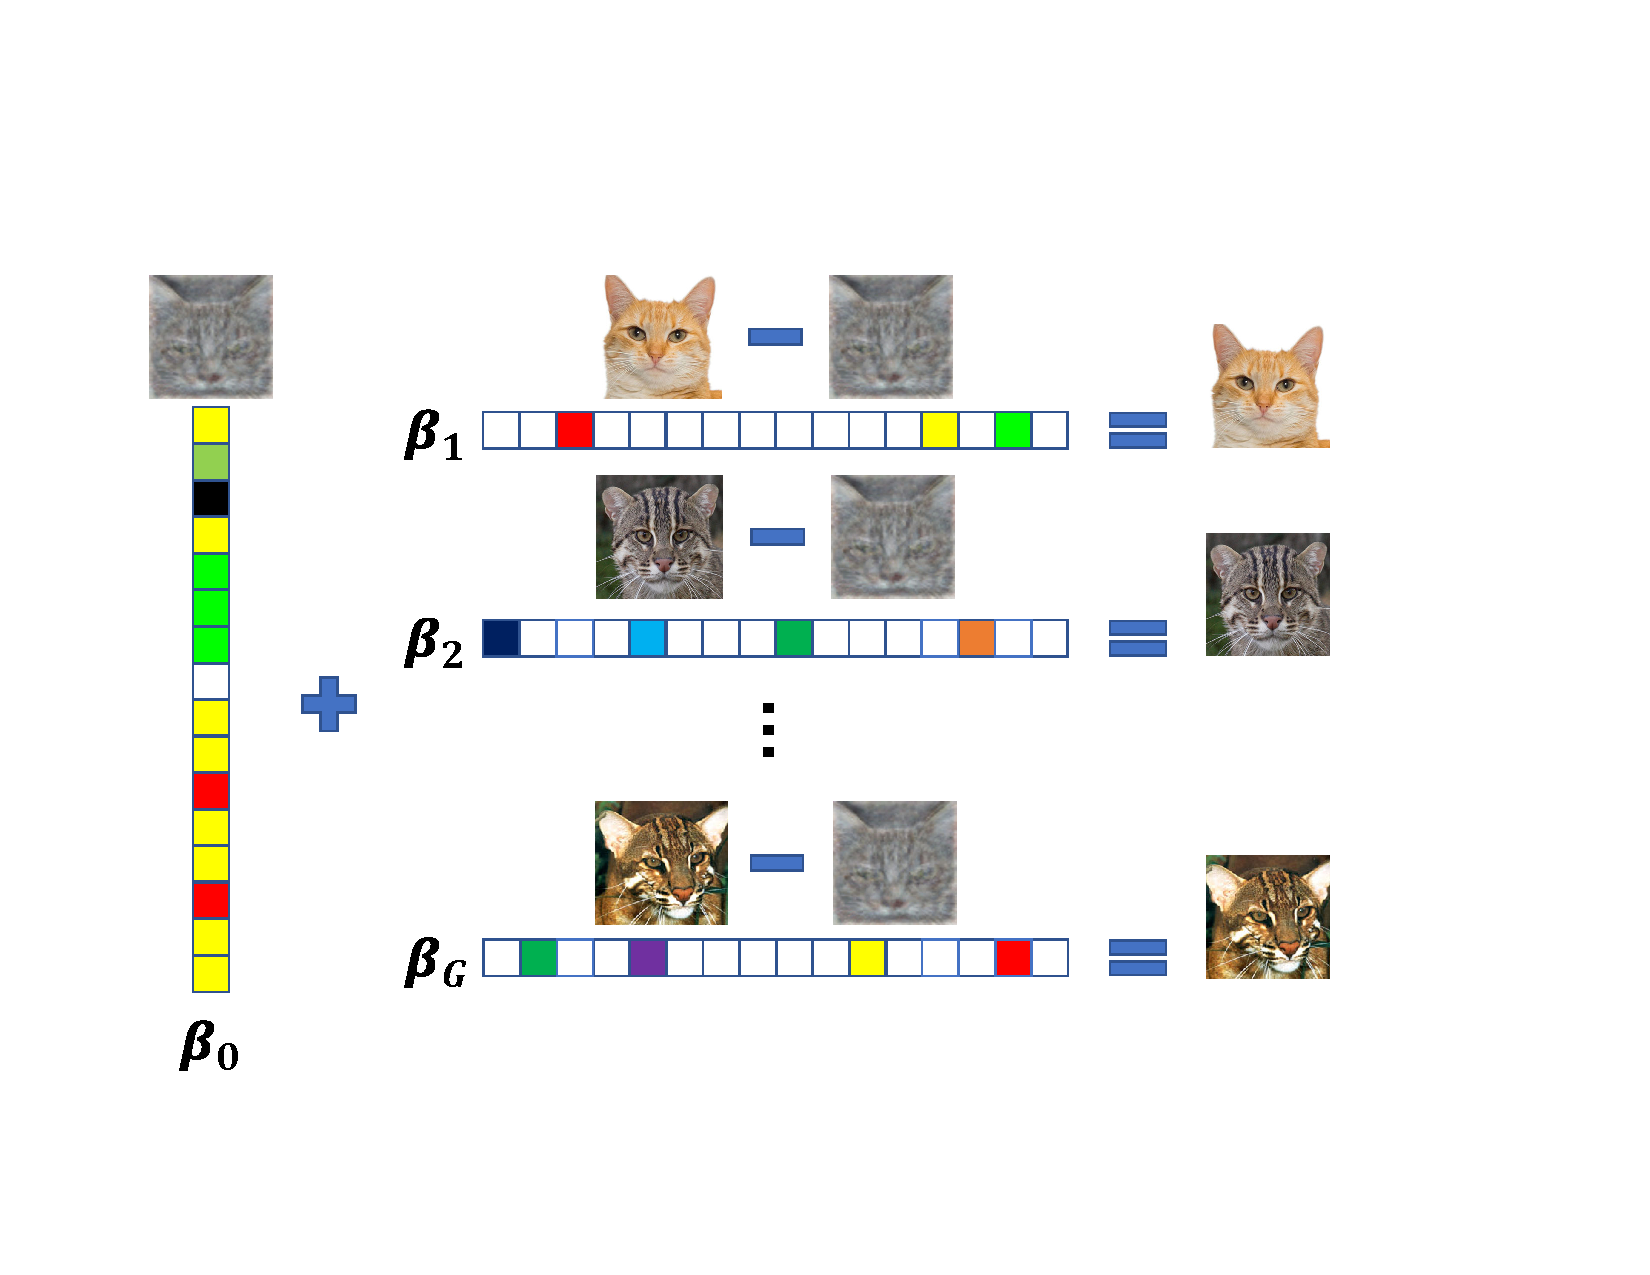
\includegraphics[height=\heightfigc]{./img/concept}
%		\parbox[b][\heightcapc][t]{1.\linewidth}{\subcaption{Data Enrichment.}\label{subfig3}}
%	\end{minipage}	\hfill
%	\begin{minipage}[b][\heightfig][t]{0.3\linewidth}\centering
%		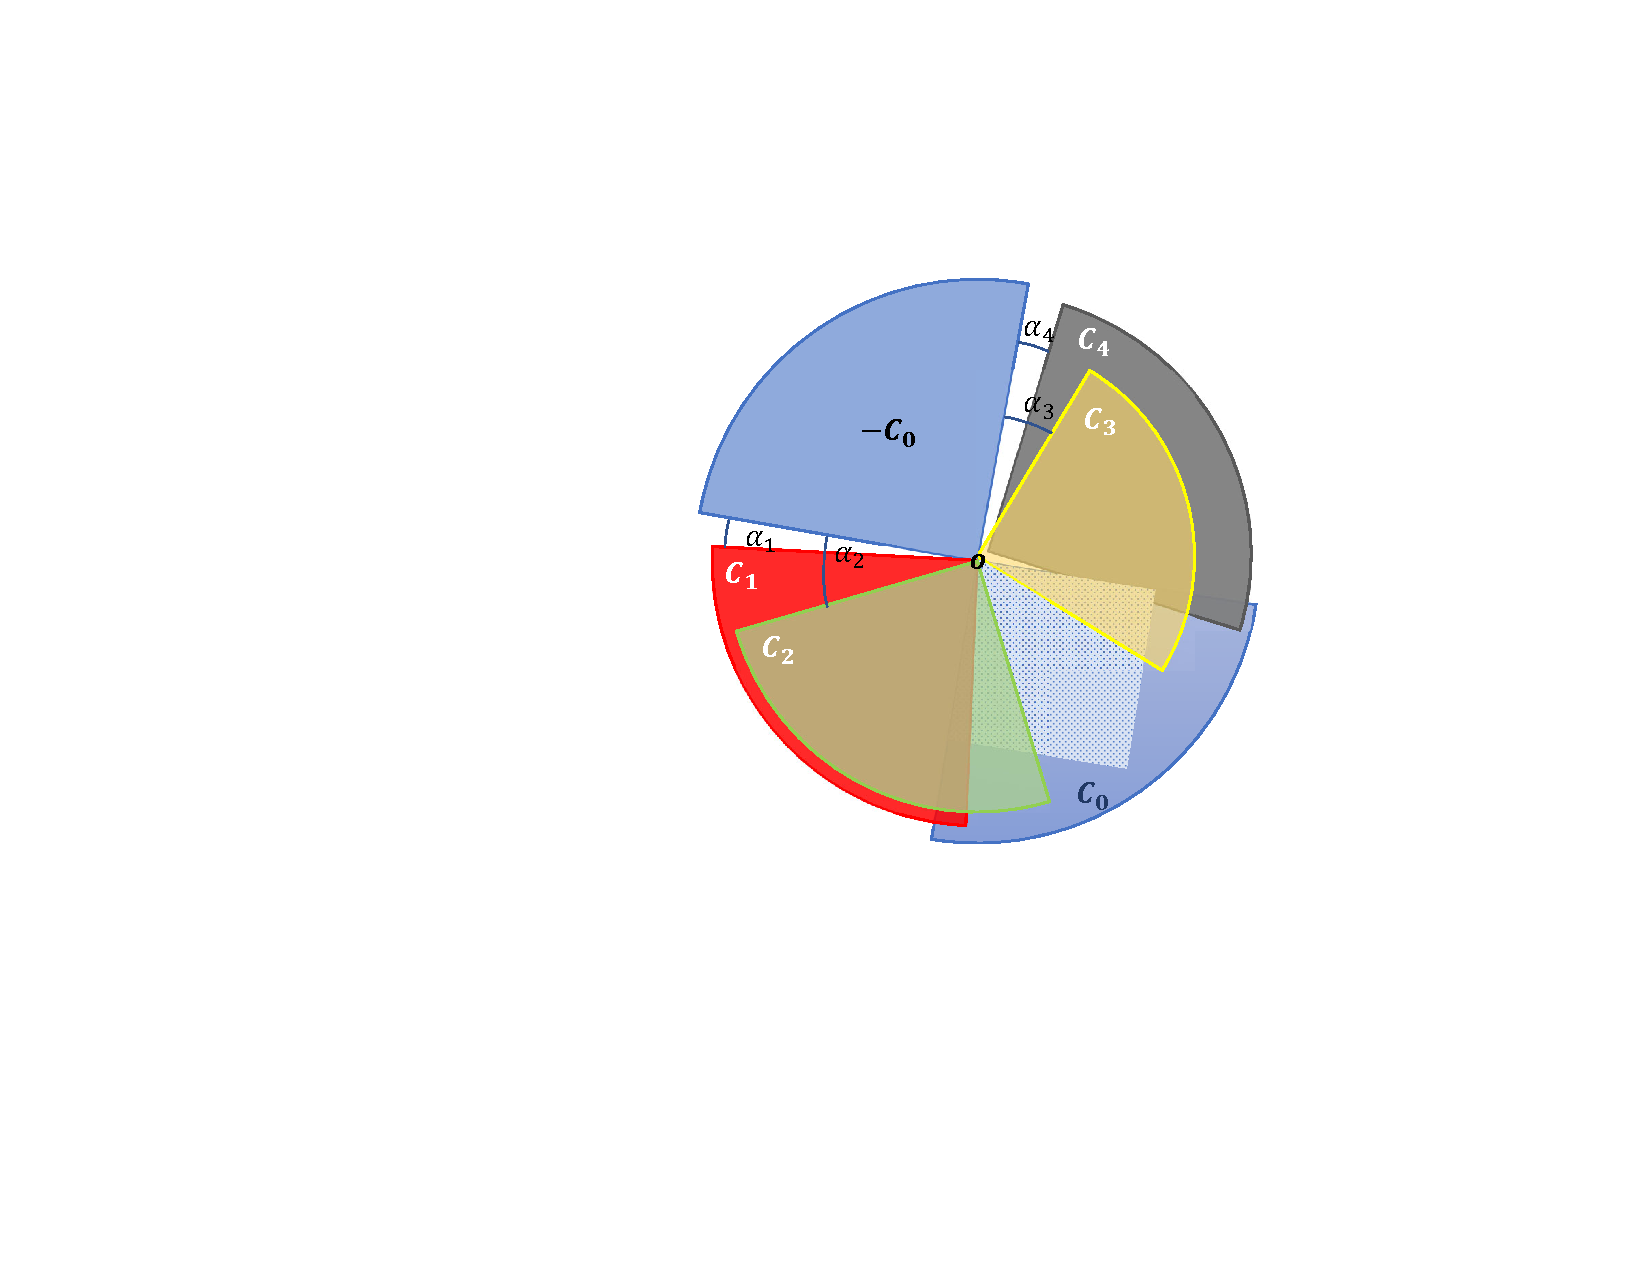
\includegraphics[height=\heightfiga]{./img/sc.pdf}
%		\parbox[b][\heightcapa][t]{1\linewidth}{\subcaption{SC}\label{subfig1}}
%		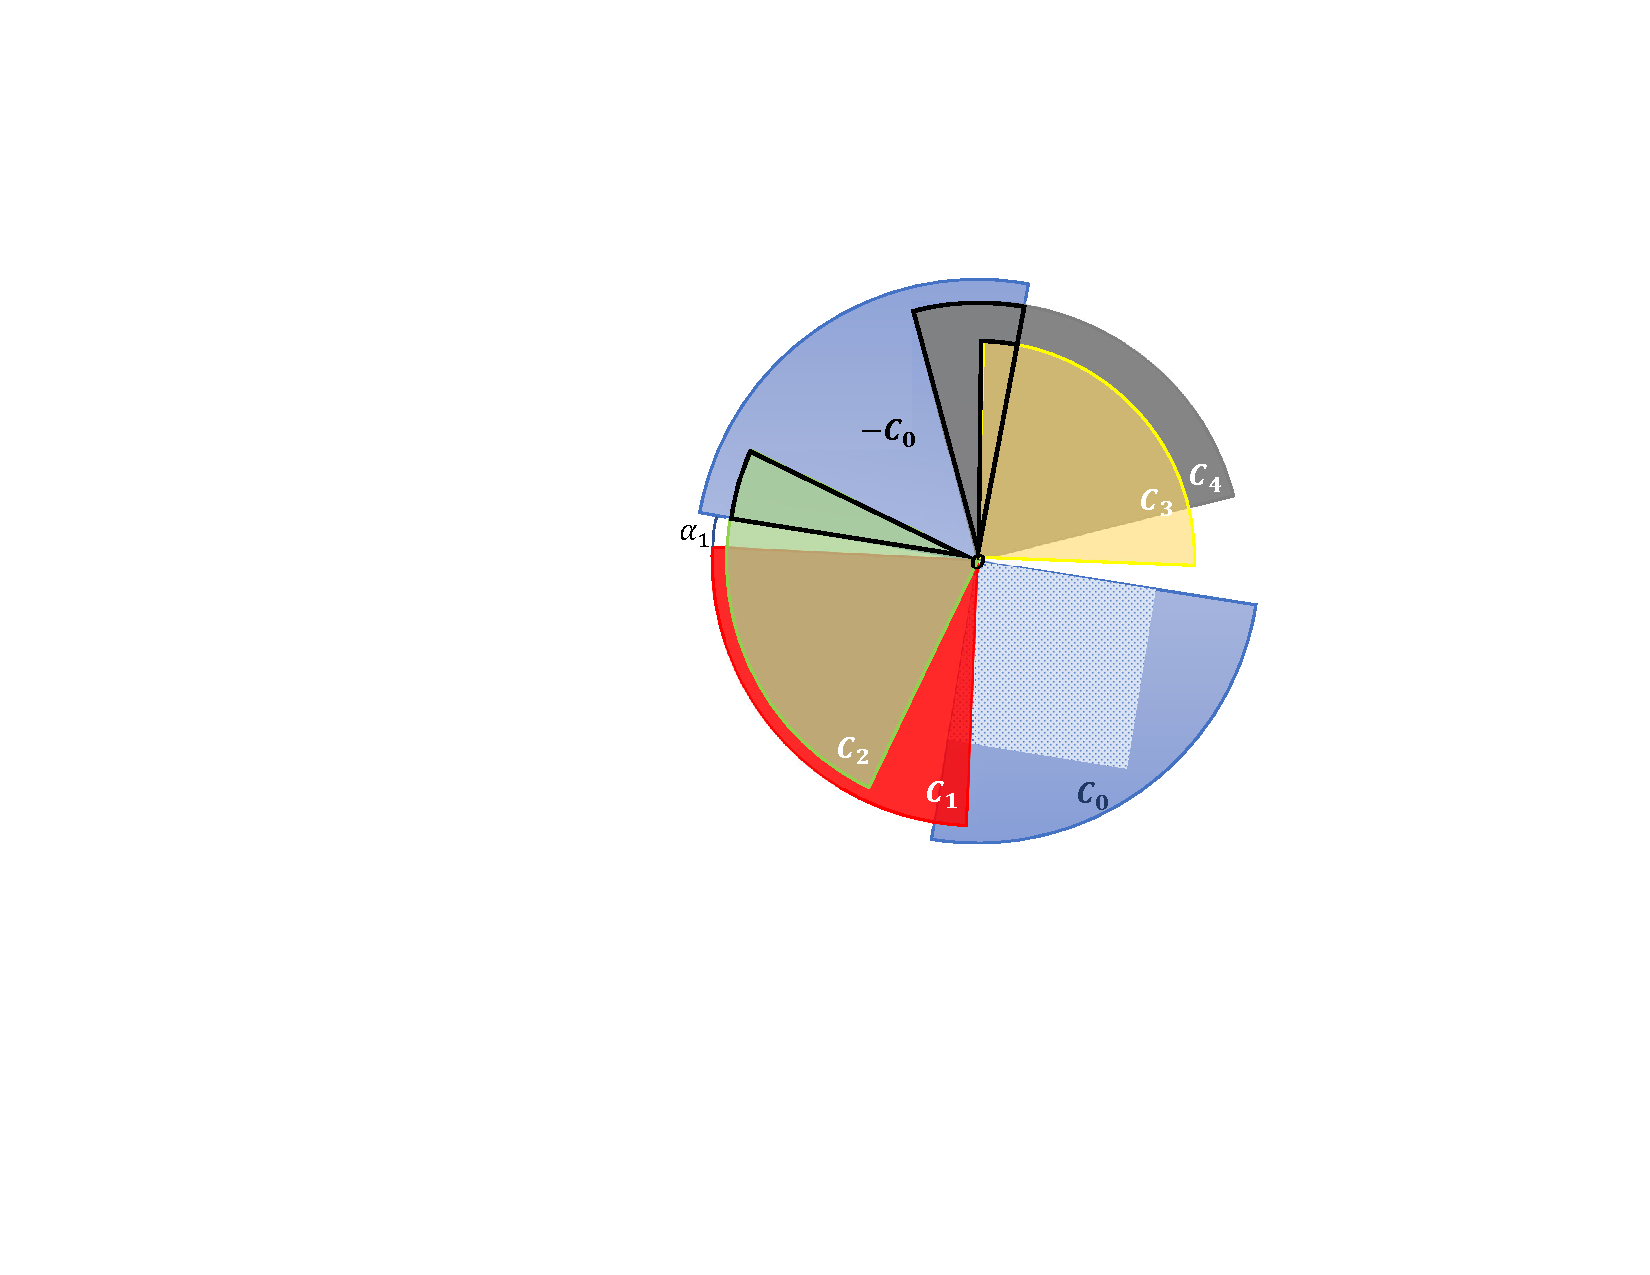
\includegraphics[height=\heightfigb]{./img/deric.pdf}
%		\parbox[b][\heightcapb][t]{1\linewidth}{\subcaption{DERIC}\label{subfig2}}
%	\end{minipage}
%	\caption{a) A conceptual illustration of data enrichment model for learning representation of  different cat species. The common parameter $\bbeta_0$ captures a \emph{generic cat} which consists of shared features among all cats. b) Our  c) Distribution of responses to Saracatinib. Note that some cell lines of both lung and blood cancers have responded to Saracatinib which makes it a good candidate for interpretability analysis.}
%	\label{fig}
%\end{figure*}
%\begin{figure}
%		\centering
%		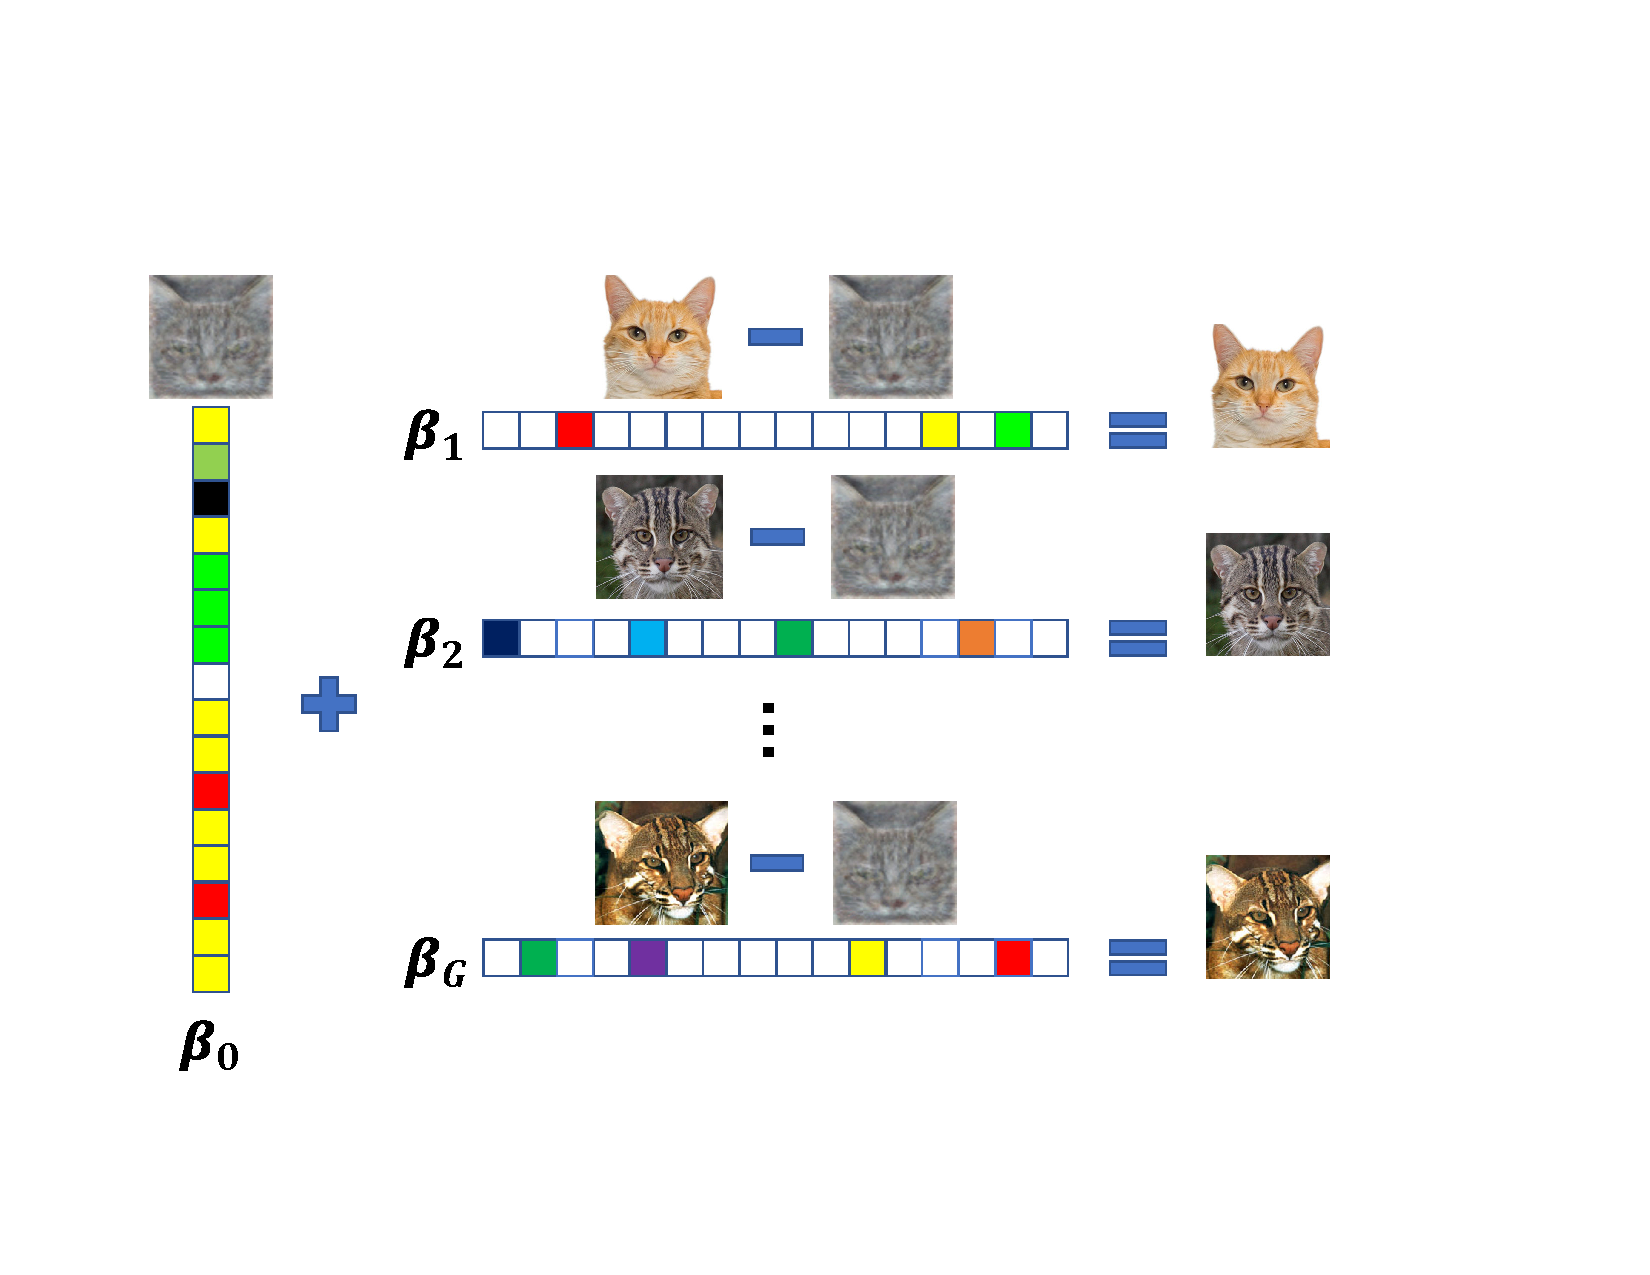
\includegraphics[scale=.25]{./img/concept.pdf}
%		\squeezeup
%		\caption{A conceptual illustration of data enrichment model for learning representation of  different cat species. The common parameter $\bbeta_0$ captures a \emph{generic cat} which consists of shared features among all cats.}
%		\label{fig:cat}		
%\end{figure}  
%{\bf Contributions:}
{\bf Notation and Preliminaries:}
We denote sets by curly $\cV$, matrices by bold capital $\V$, random variables by capital $V$, and vectors by small bold $\v$ letters.
We take $[G] = \{0, \dots, G\}$ and $[G]_\setminus = [G] \setminus \{0\}$.
%\ab{Can we use $[G]= \{1,\ldots,G\}$ and use $G \cup \{0\}$ in places where we need to include $\{0\}$? The notation will be more explicit and easier to follow.} 

Given $G$ groups and $n_g$ samples in each as $\{ \{\x_{gi}, y_{gi} \}_{i=1}^{n_g} \}_{g = 1}^G$, we can form the per group design matrix $\X_g \in \reals^{n_g \times p}$ and output vector $\y_g \in \reals ^{n_g}$.
The total number of samples is  $n = \sum_{g = 1}^{G} n_g$.
The data enriched model takes the following vector form:
\be
\label{eq:dirtymodel}
\y_g = \X_g (\bbeta _0^* + \bbeta _g^*) + \oomega_g,  \quad \forall g \in [G]_\setminus
\ee
where each row of $\X_g$ is $\x_{gi}^T$ and $\oomega_g^T = (\omega_{g1}, \dots, \omega_{gn_g})$ is the noise vector.
% are indexed with either a single number as $\v(i)$ or an index set $\cA$ as $\v_{\cA}$.
%Row $i$ of the matrix $\V$ is shown as $\v_i$ and $j$th element of the vector $\v$ is shown as $\v(j)$.
%The $(i,j)$th element of the matrix $\V$ is shown in three ways: $\V_{ij}$, $\v_i(j)$, or $v_{ij}$.
%Throughout the manuscript $c_i$ and $C_i$ are positive constants.
%We name the sample covariance of any matrix $M$ by $S_M$ vs. the actual parameter $\Sigma_M$.

%\noindent {\bf Sub-Gaussian (Sub-exponential) random variable and vector.}
A random variable $V$ is sub-Gaussian if its moments satisfies $\forall p \geq 1: (\ex |V|^p )^{1/p} \leq K_2 \sqrt{p}$.
The minimum value of $K_2$ is called the sub-Gaussian  norm of $V$, denoted by $\normth{V}{\psi_2}$ \cite{vers12}.
A random vector $\v \in \reals^p$ is sub-Gaussian if the one-dimensional marginals $\langle \v, \u \rangle$ are sub-Gaussian random variables for all $\u \in \reals^p$. The sub-Gaussian norm of $\v$ is defined \cite{vers12} as $\normth{\v}{\psi_2} = \sup_{\u \in \sphere} \normth{\langle \v, \u \rangle}{\psi_2}$.
%We abuse notation and use shorthand $\v \sim \subg(0, \Sigma_{\v}, K_{\v})$ for zero mean sub-Gaussian random vector with covariance $\Sigma_{\v}$ and sub-Gaussian norm of $K_{\v}$, although keeping in mind that no other moments, nor the exact form of the distribution function is known.
For any set $\cV \in \reals^p$ the Gaussian width of the set $\cV$ is defined as $\omega(\cV) = \ex_\g \left[ \sup_{\u \in \cV} \langle \g, \u \rangle \right]$ \cite{vershynin2018high}, where the expectation is over $\g \sim N(\0, \I_{p \times p})$, a vector of independent zero-mean unit-variance Gaussian.

%We define the minimum and maximum eigenvalues of a matrix $\M$ restricted to the set $\cA \subseteq \eS^{p-1}$ as $\lambda_{\min}(\M|\cA) = \inf_{\u \in \cA} \u^T \M \u$, and $\lambda_{\max}(\M|\cA) = \sup_{\u \in \cA} \u^T \M \u$ respectively.
%All $c_i$, $c$, and $C$ represent universal constants throughout the manuscript.
%Set $[G] = \{0, \dots, G\}$ is the index set for both shared and individual components (in the setting of data enriched model \eqref{eq:dsl}) and $[G]_\setminus = [G] - \{ 0 \}$ represents only the individual ones.


%\subsection{Contributions}
{\bf Contributions:}
We propose the following Data Enrichment (DE) estimator $\hbbe$ for recovering the structured parameters where the structure is induced by \emph{convex} functions $f_g(\cdot)$:
{\small\be
	\label{eq:super}
	\hbbe = (\hbbe_0^T, \dots, \hbbe_G^T) \in \argmin_{\bbeta _0, \dots, \bbeta _G} \frac{1}{n} \sum_{g=1}^{G} \norm{\y_g - \X_g (\bbeta _0 + \bbeta _g)}{2}^2,
	\\ \nr
	\text{s.t.} \quad \forall g \in [G]:f_g(\bbeta _g) \leq f_g(\bbeta _g^*).
\ee}
%We are investigating the conjecture that the pooled data from all groups will facilitate estimation of the common parameter $\bbeta_0^*$ in both samples complexity and error-bound rate regards.
%In our work, we explicitly answer these questions as follows:
We present several statistical and computational results for the DE estimator \eqref{eq:super} of the data enriched model:
\begin{itemize}[leftmargin = .4cm]
	\item The DE estimator \eqref{eq:super} succeeds if a geometric condition that we call \emph{Data EnRichment Incoherence Condition} (DERIC) is satisfied, Figure \ref{fig:deric}. Compared to other known geometric conditions in the literature such as structural coherence \cite{guba16} and stable recovery conditions \cite{mctr13}, DERIC is a weaker condition, Figure \ref{fig:sc}.
	\item Assuming DERIC holds, we establish a high probability non-asymptotic bound on the weighted sum of parameter-wise estimation error, $\ddelta_g = \hbbe_g - \bbeta_g^*$ as:
	\be
	\label{eq:errorsum}
	\sum_{g=0}^{G}  \sqrt{\frac{n_g}{n}} \|\ddelta_g\|_2 \leq  \gamma O\left(\frac{\max_{g \in [G]} \omega(\cC_g \cap \sphere)}{\sqrt{n}}\right),
%	\sum_{g=0}^{G}  \sqrt{\frac{n_g}{n}} \|\ddelta_g\|_2 \leq  C \gamma \frac{\max_{g \in [G]} \omega(\cC_g \cap \sphere) + \sqrt{\log (G+1)}}{\sqrt{n}},
	\ee
	where $n_0 \triangleq n$ is the total number of samples, $\gamma \triangleq \max_{g \in [G] } \frac{n}{n_g}$ is the \emph{sample condition number}, and $\cC_g$ is the error cone corresponding to $\bbeta_g^*$ exactly defined in Section \ref{sec:esti}.
	To the best of our knowledge, this is the first statistical estimation guarantee for the data enrichment.%ed model.
	%Gaussian width of a set $\cS$ is $\omega(\cS) = \ex_\g \left[ \sup_{\u \in \cS} \langle \g, \u \rangle \right]$. Gaussian width has been a standard tool for capturing the complexity of high-dimensional problems \cite{venkat12}.
	
%	Similar to previous works, we make a geometric assumption regarding the relation $\cC_g$s in each individual problem which is known as Structural Coherence assumption \cite{guba16, trop15}.
%	\item The general bound of \eqref{eq:errorsum} entails the following bounds for specific parameters:
%	\be
%	\nr
%	\forall g \in [G]: \norm{\ddelta_g}{2} \leq c \gamma \frac{\max_{g \in [G]} \omega(\cC_g \cap \sphere) + c\sqrt{\log G}}{\sqrt{n_g}}
%	\ee
%	Observe that $l_2$-norm of the estimation error for the common parameter decays as $1/\sqrt{n}$, similar to the well-studied high dimensional regression case \cite{venkat12, banerjee14}.
%	So the common parameter's estimator exploits all of the pooled data to reduce its error.
	\item We also establish the sample complexity of the DE estimator for all parameters as $\forall g \in [G]: n_g = O(\omega(\cC_g \cap \sphere))^2$. We emphasize that our result proofs that the recovery of the common parameter $\bbeta_0$ by DE estimator benefits from \emph{all} of the $n$ pooled samples.
	\item We present an efficient projected block gradient descent algorithm \emph{\dc}, to solve DE's objective \eqref{eq:super} which converges geometrically to the statistical error bound of \eqref{eq:errorsum}. To the best of our knowledge, this is the first rigorous computational result for the high-dimensional data-enriched regression.
%	\item We illustrate promising empirical performance of the model on synthetic data as well as on the problem of finding bio-markers associated with drug sensitivity of cell lines from different cancer types, where the support of estimated individual parameters $\text{supp}(\hbbe_g)$ for each cancer type $g$ represents a different set of bio-markers per cancer type.
\end{itemize}

%The rest of this paper is organized as follows:
%%First, we present a review of the related works in Section \ref{relwork}.
%First, we characterize the error set of our estimator and provide a deterministic error bound in Section \ref{sec:esti}.
%Then in Section \ref{sec:re}, we discuss the restricted eigenvalue condition and calculate the sample complexity required for the recovery of the true parameters by our estimator under DERIC condition.
%We close the statistical analysis in Section \ref{sec:error} by providing non-asymptotic high probability error bound for parameter recovery.
%We delineate our geometrically convergent algorithm, \dc{} in Section \ref{sec:opt} and finally supplement our work with synthetic and real experiments in Sections \ref{sec:expds} and \ref{realexp}.

\begin{figure}[t!]
	\centering
	\begin{subfigure}[t]{0.22\textwidth}
		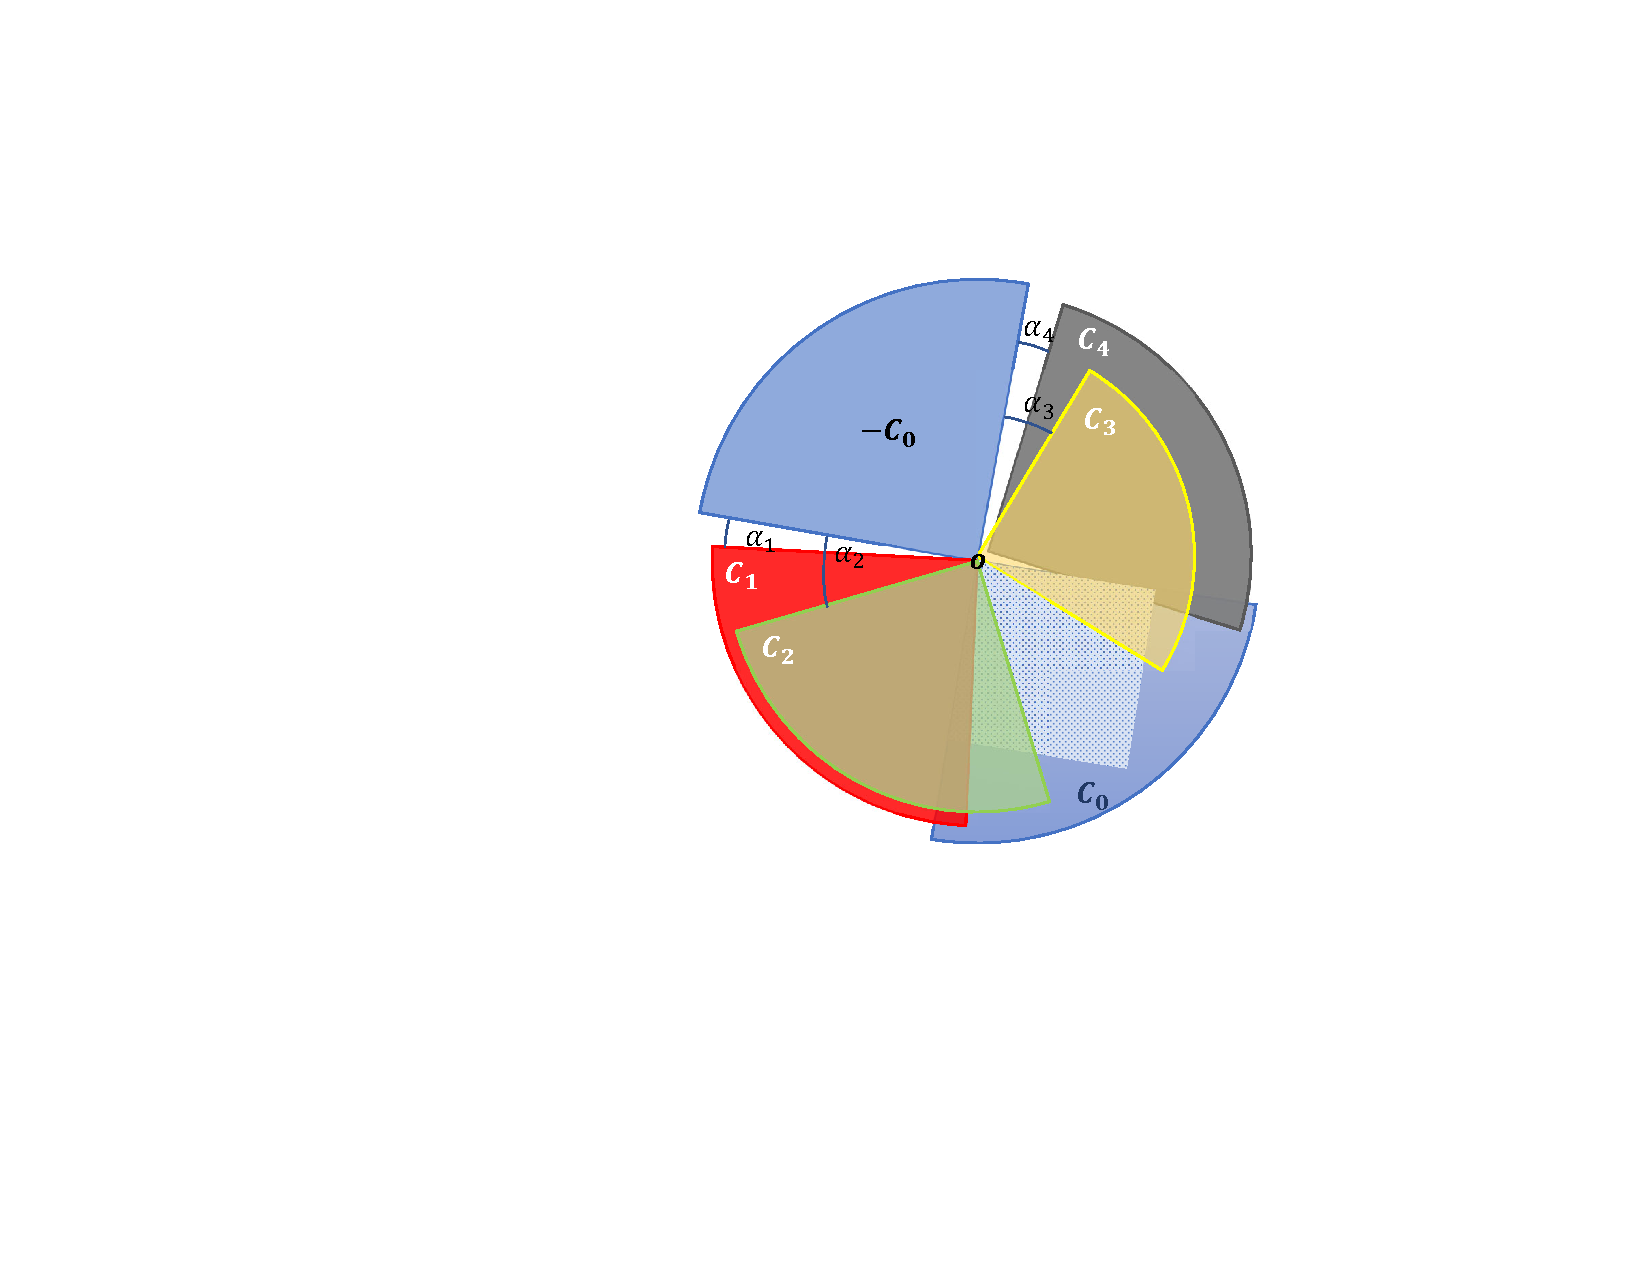
\includegraphics[width=\textwidth]{./img/sc.pdf}
		\caption{Structural Coherence (SC) condition.}\label{fig:sc}
	\end{subfigure} 
	~
	\begin{subfigure}[t]{0.22\textwidth}
		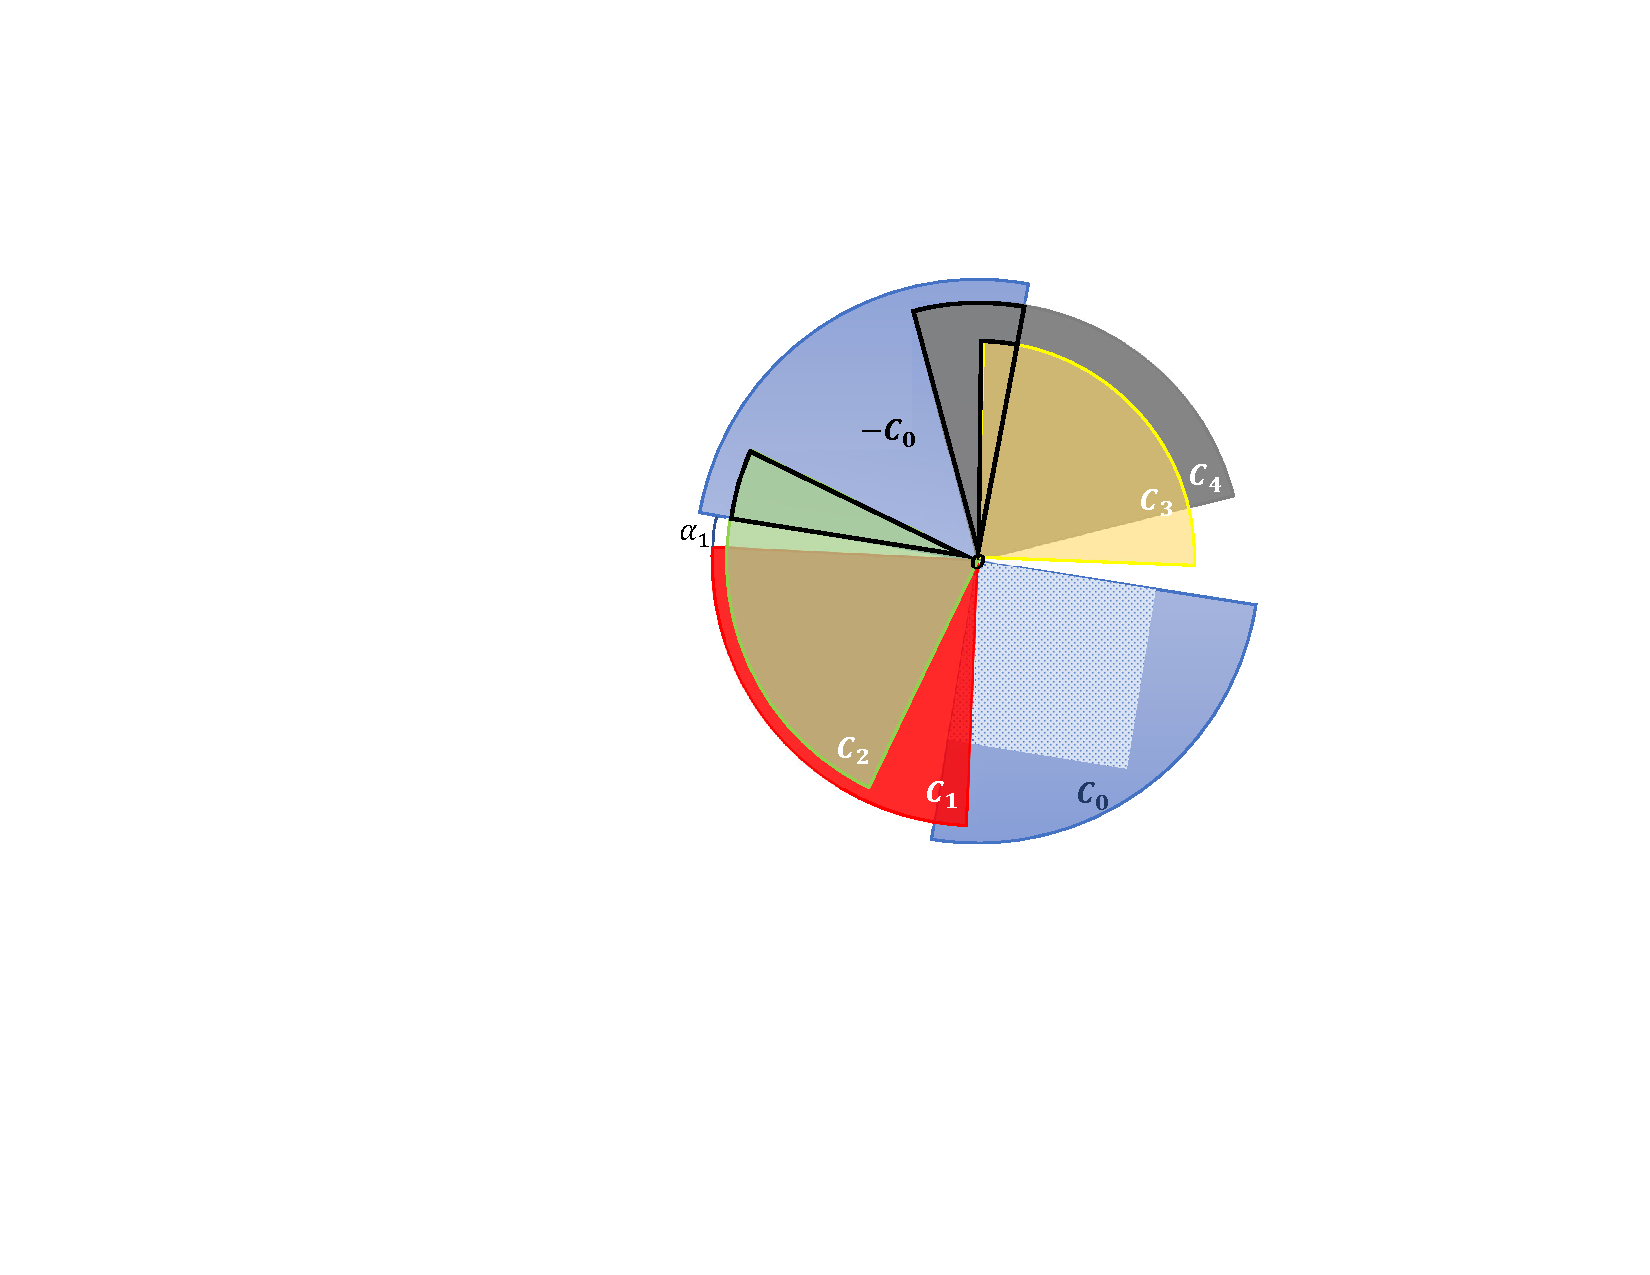
\includegraphics[width=1.04\textwidth]{./img/deric.pdf}
		\caption{Data EnRichment Incoherence Condition (DERIC). }
		\label{fig:deric}
	\end{subfigure}
	\squeezeup
	\caption{a) State of the art condition for recovering common and individual parameters in superposition models where $\cC_g = \text{Cone}(\cE_g)$ are error cones and $\cE_g = \left\{\ddelta_g | f_g(\bbeta _g^* + \ddelta_g) \leq f_g(\bbeta _g^*)\right\}$ are the error sets for each parameter $\bbeta^*_g \in [G]$ \cite{guba16} b) Our more relaxed recovery condition which allows \emph{arbitrary non-zero fraction } of the error cones of individual parameters intersect with $-\cC_0$.}
	\label{fig syn2}
\end{figure}




%In machine learning, limited training samples in many applications such as medicine has led to a collection of learning methods known as \emph{Multi-Task Learning} (MLT) \cite{Zhang2017-rm}. In supervised parametric setting such as regression, the relation between tasks is captured by explicitly modeling the relation between their parameters. One class of such modeling assumes that the parameter matrix 


	
	%\section{Related Work}
%\label{relwork}
%
%It is worth noting that data sharing framework has tight connections to multi-task learning 
%
%\subsection{Connection to multitask learning and Rubin's causality}

%Like any high dimensional model, questions about the data sharing model concerns sample complexity required for recovering the parameters and the non-asymptotic rate of estimation error.
%Here, the more interesting question is about the common parameter. 
%Is the sample complexity of $\bbeta_0^*$ depends on the data of all groups? 
%What about the rate of the error bound? 
%In other words, we are investigating the conjecture that the pooled data from all groups will facilitate estimation of the common parameter in both samples complexity and error bound rate regards. 
%In our work, we explicitly answer these questions.
	
	\section{The Data Enrichment Estimator}
\label{sec:esti}
%Given $G$ group and $n_g$ samples in each one as $\{ \{\x_{gi}, y_{gi} \}_{i=1}^{n_g} \}_{g = 1}^G$, we can form the per group design matrix $\X_g \in \reals^{n_g \times p}$ and output vector $\y_g \in \reals ^{n_g}$.
%The total number of samples is  $n = \sum_{g = 1}^{G} n_g$.
%The data enriched model takes the following vector form:
%\be
%\label{eq:dirtymodel}
%\y_g = \X_g (\bbeta _0^* + \bbeta _g^*) + \oomega_g,  \quad \forall g \in [G]_\setminus
%\ee
%where each row of $\X_g$ is $\x_{gi}^T$ and $\oomega_g^T = (\omega_{g1}, \dots, \omega_{gn_g})$ is the noise vector. %consists of i.i.d. centered unit-variance sub-Gaussian elements with $\normth{\omega_{gi}}{\psi_2} \leq K$.
%Note that,
%The common parameter among all groups is $\bbeta _0^*$ and the individual parameter of the group $g$ is $\bbeta _g^*$.
%Beside a deterministic error bound presented in Section \ref{sec:deter} our other results are probabilistic.
%We focus on independent isotropic sub-Gaussian random vectors $\x_{gi}$ where $\normth{\x_{gi}}{\psi_2} \leq k$ and $\ex \x_{gi}^T \x_{gi}  = \I_{p \times p}$.

%\subsection{The Estimator}
A compact form of our proposed DE estimator \eqref{eq:super} is:% optimization problem as: %:
\be
\label{eq:compact}
\hbbe \in \argmin_{\bbeta } \frac{1}{n} \norm{\y - \X \bbeta }{2}^2, \forall g \in [G]:f_g(\bbeta_g ) \leq f_g(\bbeta^*_g),
\ee
where $\y  = (\y^T_1, \dots \y^T_G)^T \in \reals^n$,  $\bbeta  = ({\bbeta _0}^T, \dots, {\bbeta _G}^T)^T \in \reals^{(G+1)p}$ and
\be
\label{eq:x}
\X =
\begin{pmatrix}
	\X_1     & \X_1      & 0      	   & \cdots & 0 \\
	\X_2     & 0       	 & \X_2        & \cdots & 0 \\
	\vdots 	 & \vdots  	 & \ddots 	   & \cdots & \vdots  \\
	\X_G     & 0       	 & \cdots 	   & \cdots & \X_G
\end{pmatrix}
\in \reals^{n \times (G+1)p}~.
\ee
%For simplicity, during steps of the analysis we denote $\X = [\X_0 \enskip \D]$ which is the concatenation of $\X_0 \in \reals^{n \times p}$ that represents the \emph{whole} design matrix consisting of all data points as rows and $\D \in \reals^{n \times pG}$ which is the \emph{diagonal} part of the $\X$ where all $\X_g$s are on the diagonal.
%Following this convention, we refer to total number of samples $n$ as $n_0$ in our analysis.

\ab{Give at least 2 specific examples, e.g., a sparse+sparse for vector estimation, and a low-rank + sparse for matrix estimation. And we want to carry these examples through
the technical results, e.g., see the Chen-Banerjee NIPS 2015 paper.}

\begin{example}
This is an example
\end{example}

\subsection{Error Set and Deterministic Error Bound}
\label{sec:deter}
\ab{Unless we need a second subsection, drop this subsection heading -- its unusual to have one subsection in a section.}

Consider the group-wise estimation error $\ddelta_g = \hbbe_g - \bbeta^*_g$.
Since $\hbbe_g = \bbeta ^*_g + \ddelta_g$ is a feasible point of \eqref{eq:compact}, the error vector $\ddelta_g$ will belong to the following restricted error set:% which is the set of all descent directions at $\bbeta _g^*$ on $f_g(\cdot)$ :
\be
%\nr
\cE_g = \left\{\ddelta_g | f_g(\bbeta _g^* + \ddelta_g) \leq f_g(\bbeta _g^*)\right\}, \quad g \in [G]~.
\ee
We denote the cone of the error set as $\cC_g \triangleq \text{Cone}(\cE_g)$ and the spherical cap corresponding to it as $\cA_g \triangleq \cC_g \cap \sphere$.
%Subsequently, we define the following family of sets:
%\be
%\nr
%\cH_l &=& \left\{ \ddelta = (\ddelta_0^T, \dots, \ddelta_G^T)^T \Big| \forall g \in [G]: \ddelta_g \in \cC_g, 0 < l \leq \sum_{g=0}^{G} \sqrt{\frac{n_g}{n}} \norm{\ddelta_g}{2} \leq 1 \right\}, %\label{setH}
%\ee
%where $0 < l < 1$ indexes the family.
Consider the set $\cC = \{ \ddelta = (\ddelta_0^T, \dots, \ddelta_G^T)^T \Big| \ddelta_g \in \cC_g \}$, following two subsets of $\cC$ play key roles in our analysis:
\be
%\nr
\cH  &\triangleq&  \Big\{ \ddelta \in \cC \big| \sum_{g=0}^{G} {\frac{n_g}{n}} \norm{\ddelta_g}{2} = 1 \Big\}~, %\label{setH}
\\ %\nr
\bcH &\triangleq&  \Big\{ \ddelta \in \cC \big| \sum_{g=0}^{G} \sqrt{\frac{n_g}{n}} \norm{\ddelta_g}{2} = 1 \Big\}~. %\label{setH}
\ee
Starting from the optimality of $\hbbe = \bbeta ^* + \ddelta$ as $\frac{1}{n}\norm{\y - \X \hbbe}{2}^2 \leq \frac{1}{n} \norm{\y - \X \bbeta ^*}{2}^2$, we have:
%\be
%\label{eq:optimality}
%\frac{1}{n}\norm{\X \ddelta}{2}^2 &\leq& \frac{1}{n}2\oomega^T \X\ddelta
%\ee
$\frac{1}{n}\norm{\X \ddelta}{2}^2 \leq \frac{1}{n}2\oomega^T \X\ddelta$
where $\oomega = [\oomega_1^T, \dots, \oomega_G^T]^T \in \reals^n$ is the vector of all noises.
Using this basic inequality, we can establish the following deterministic error bound.
\begin{theorem}
	\label{theo:deter}
	For the proposed estimator \eqref{eq:compact}, assume there exist $0 < \kappa \leq \inf_{\u \in \cH} \frac{1}{n} \norm{\X \u}{2}^2$. Then, for the sample condition number $\gamma = \max_{g \in [G]_{\setminus}} \frac{n}{n_g}$, the following deterministic upper bounds holds:
	\be
	\nr
	\sum_{g=0}^{G} \sqrt{\frac{n_g}{n}} \norm{\ddelta_g}{2} \leq \frac{2{\gamma}\sup_{\u \in \bcH}\oomega^T \X \u}{n\kappa}~. %\nr	
	\ee
\end{theorem}

\ab{Adding a remark -- these will make it easier for the reader. This specific remark can be dropped as needed.}

\begin{remark}
Consider the setting where $n_g = \Theta(\frac{n}{G})$ so that each group has approximately $\frac{1}{G}$ fraction of the samples. Then, $\gamma = \Theta(G)$ and hence
\beq
\frac{1}{G} \sum_{g=0}^G \| \delta_g \|_2 \leq O( G^{1/2} ) \frac{\sup_{\u \in \bcH}\oomega^T \X \u}{n}~.
\eeq
\end{remark}

%We define $\gamma_g = \norm{\ddelta_g}{2}$ and for $\ddelta \in \cH$ we have $\sum_{g = 0}^{G} \gamma_g = 1$.
%We are interested in the following RE condition:
%\begin{remark}
%	As we show in the following, the lower bound $\kappa  < \inf_{\u \in \cC} \norm{\X \u}{2}^2 $, holds even for the larger set $\cC \supset \cA$, which is an interesting result.	On the other hand, if we work with the set $\cC$ in the upper bound, the bound becomes loose.
%	Therefor, we focus on the set $\cA$ to get the tighter upper bound.
%\end{remark}

	
	\section{Restricted Eigenvalue Condition}
\label{sec:re}
The main assumptions of Theorem \ref{theo:deter} is known as Restricted Eigenvalue (RE) condition in the literature of high-dimensional statistics \cite{banerjee14, nrwy12, raskutti10}:
$\inf_{\u \in \cH} \frac{1}{n} \norm{\X \u}{2}^2 \geq \kappa > 0.$
%\be
%\label{eq:recond}
%\inf_{\u \in \cH} \frac{1}{n} \norm{\X \u}{2}^2 \geq \kappa > 0.
%\ee
The RE condition posits that the minimum eigenvalues of the matrix $\X^T \X$ in directions restricted to $\cH$ is strictly positive.
In this section, we show that for the design matrix $\X$ defined in \eqref{eq:x}, the RE condition holds with high probability under a suitable geometric condition we call {\em Data EnRichment Incoherence Condition} (DERIC) and for enough number of samples.
We precisely characterize total and per-group sample complexities required for successful parameter recovery.
For the analysis, similar to existing work \cite{guba16, mend15, trop15}, we assume the design matrix to be isotropic sub-Gaussian.\footnote{Extension to an-isotropic sub-Gaussian case is straightforward by techniques developed in \cite{banerjee14, ruzh13}.}
\begin{definition}
	\label{def:obs}
	We assume $\x_{gi}$ are i.i.d. random vectors from a non-degenerate zero-mean, isotropic sub-Gaussian distribution. In other words, $\ex [\x] = 0$, $\ex [\x^T \x] = \I_{p \times p}$, and $\normth{\x}{\psi_2} \leq k_x$.	
As a consequence, $\exists \alpha > 0$ such that $\forall \u \in \sphere$ we have $ \ex|\langle \x, \u \rangle| \geq \alpha$. Further, we assume noise $\w_{gi} $ are i.i.d.
zero-mean, unit-variance sub-Gaussian with $\normth{\w_{gi}}{\psi_2} \leq k_w$.
\end{definition}

\subsection{Geometric Condition of Recovery}
Unlike standard high-dimensional statistical estimation, for RE condition to be true, parameters of superposition models need to satisfy geometric conditions which limits the interaction of parameters with each other to make sure that recovery is possible. In this section, we elaborate our sufficient geometric condition for recovery and compare it with state-of-the-art condition for recovery of superposition models. 

To intuitively illustrate the necessity of such a geometric condition, consider the simplest superposition model i.e., $\bbeta^*_0 + \bbeta^*_g$. Without any restriction on parameter interactions, any estimates such that $\hbbe_0 + \hbbe_g = \bbeta^*_0 + \bbeta^*_g$ are valid ones. To avoid such trivial solutions two error cones need to satisfy $\ddelta_g \neq -\ddelta_0$. In general, the RE condition of individual superposition models can be established under the so-called Structural Coherence (SC) condition \cite{guba16, mctr13} which is the generalization of this idea for superposition of multiple parameters as $\sum_{g = 0}^{G} \bbeta^*_g$.
 
\begin{definition}[Structural Coherence (SC) \cite{guba16, mctr13}] \label{scc}
	Consider a superposition model of the form $y = \x^T \sum_{g = 0}^{G} \bbeta^*_g + w$. The SC condition requires that
	\be 
	\nr 
	\forall \ddelta_g \in \cC_g, \exists \lambda \quad  \text{s.t.}  \quad \norm{\sum_{g = 0}^{G} \ddelta_g}{2} \geq  \lambda \sum_{g = 0}^{G}  \norm{\ddelta_g}{2},
	\ee  
	and leads to the corresponding RE condition for the superposition model.
\end{definition}

\begin{remark}
	Note that the SC condition is satisfied if none of the individual error cones $\cC_g$ intersect with the inverted error cone $-\cC_0$ \cite{guba16, trop15}, i.e., $\forall g, \alpha_g > 0$ in Figure \ref{fig:sc} where 
	\be 
	\nr 
	\cos(\alpha_g) = \sup_{\ddelta_0 \in \cC_0, \ddelta_g \in \cC_g} -\langle \ddelta_0/\norm{\ddelta_0}{2}, \ddelta_g/\norm{\ddelta_g}{2} \rangle.
	\ee
\end{remark}
Next, we introduce DERIC, a considerably weaker geometric condition compared to SC which leads to recovery of all parameters in the data enriched model. 
\begin{definition}[Data EnRichment Incoherence Condition (DERIC)]  \label{incodef}
	There exists a non-empty set $\cI\subseteq [G]$ of groups where for some scalars $0 < \ratio\leq 1$ and $\lamin>0$ the following holds:
	\begin{enumerate}
		\item $\sum_{i\in \cI} n_i\geq \lceil \ratio n\rceil$.
		\item $\forall i \in \cI$, $\forall \ddelta_i \in \cC_i$, and $\ddelta_0\in\cC_0$: $\norm{\ddelta_i+\ddelta_0}{2}\geq \lamin (\norm{\ddelta_0}{2}+\norm{\ddelta_i}{2})$
	\end{enumerate}
	Observe that $0 < \lamin,\ratio\leq 1$ by definition.
\end{definition}
%\ab{why would $\bar{\rho}=0$ work? also, can $\cI$ be empty? pls update as needed} 

%\ab{add a remark -- so the reader can follow what we are saying}

%\ab{It will be great to have a Figure showing the difference between SC and DERIC.}

\begin{remark}
Comparing to the SC conditions, DERIC holds even if only one of the $\cC_g$s does not intersect with $-\cC_0$. More specifically, DERIC holds if $\exists g, \alpha_g > 0$ in Figure \ref{fig:deric}. Therefore, instead of SC stringent geometric condition, DERIC allows $-\cC_0$ to intersect with an arbitrarily large fraction of the $\cC_g$ cones and as the number of intersections increases, our final error bound becomes looser.
\end{remark}

\subsection{Sample Complexity}
The SC condition on each individual problem fails to utilize the true coupling structure in the data enriched model, where $\bbeta^*_0$ is involved in all groups. In fact, below we show, using SC on each individual model leads to radically pessimistic estimates of the sample complexity for $\bbeta^*_0$ recovery.
\begin{prop}
	\label{prop:super}
	Assume observations distributed as defined in Definition \ref{def:obs} and pair-wise SC conditions are satisfied.  Consider each superposition model \eqref{eq:dirtymodel} in isolation; to recover the common parameter $\bbeta _0^*$ requires at least one group $i$ to have $n_i = O(\omega^2(\cA_0))$. 
	To recover the rest of individual parameters, we need $\forall g \neq i: n_g = O(\omega^2(\cA_g))$ samples. 
	%Recovering the individual parameter $\bbeta^*_g$ needs at least $n_g =  O((\max_{g \in [G]}\omega(\cA_g) + \sqrt{\log 2})^2)$ samples in the group.
\end{prop}
In other words, by separate analysis of superposition estimators at least one problem needs to have sufficient samples for recovering the common parameter $\bbeta_0$ and therefore the common parameter recovery does not benefit from the pooled $n$ samples.
But given the nature of coupling in the data enriched model, we hope to be able to get a better sample complexity specifically for the common parameter $\bbeta_0$.

%\ab{Not sure if I follow this. Assume $g=1$ has sufficient samples, i.e., $n_1 \geq c \omega^2(\cA_0)$. Then, the estimator would proceed in two steps: first, estimate $\beta_0,\beta_1$
%from the first problem; then, use the estimated $\beta_0$ in the other problems to estimate $\beta_2,\ldots,\beta_G$. With such an estimator, we need $n_g \geq c \omega^2(\cA_g), g=2,\ldots,G$.
%So only one problem needs to have sufficient samples.}


%
%Therefore, we have a set of coupled superposition models, and the goal is to estimate their parameters.
%%Another similar model is the one used in \cite{jrsr10}, but the authors are not emphasizing on a distinct common component.
%%As mentioned in Section \ref{sec:introds} the data enriched model can be think of as a coupled set of superposition models.
%The straightforward way to get the sample complexity for satisfying the RE condition is to use results from the superposition literature directly.
%To this end, we need to introduce some preliminary concepts that both previous works and ours build upon.
%
%Secondly to establish the RE condition, shared signal should satisfy an incoherence condition under which we prevent trivial solutions such as $\ddelta_g=-\ddelta_0$ for all $g \in [G]_\setminus$.

 Using DERIC and the small ball method \cite{mend15}, a recent tool from empirical process theory in the following theorem, we get a better sample complexity required for satisfying the RE condition:
\begin{theorem}
	\label{theo:re}
%	Let $\x_{gi}$s be iid, zero-mean, non-degenerate, sub-Gaussian random vector with $\ex [\x_{gi}^T \x_{gi}] = \I_{p \times p}$ and $\vertiii{\x_{gi}}_{\psi_2} \leq k$.
	Let $\x_{gi}$s	be random vectors defined in Definition \ref{def:obs}.
%	Assume that the pair-wise SC conditions of \eqref{def:sc} hold for $\cC_g$s.
	Assume DERIC condition of Definition \ref{incodef} holds for error cones $\cC_g$s and $\rinc=\lamin\ratio/3$.
	Then, for all $\ddelta \in \cH$, when we have enough number of samples as $\forall g \in [G]_{\setminus}: n_g \geq m_g = O(k^6 \alpha^{-6} \rinc^{-2} \omega(\cA_g)^2)$, with probability at least $1 - e^{-n \kappa_{\min}/4}$  we have:
	%as characterized where $-\langle \oomega \ddelta_0 , \D \ddelta_{1:G} \rangle \leq \epsilon \norm{\oomega \ddelta_0}{2} \norm{\D \ddelta_{1:G}}{2}$, therefore we have the following:
	\be
	\nr
	\inf_{\ddelta \in \cH} \frac{1}{\sqrt{n}} \norm{\X \ddelta}{2} &\geq& \frac{\kappa_{\min}}{2}
	\ee
	where $\kappa_{\min} = \min_{g\in [G]_\setminus} C \rinc \frac{\alpha^3}{k^2}  - \frac{2 c_g k \omega(\cA_g)}{\sqrt{n_g}}$ and $\kappa = \frac{\kappa_{\min}^2}{4}$ is the lower bound of the RE condition.
\end{theorem}

\begin{example}
	{\bf ($L_1$-norm)} The Gaussian width of the spherical cap of a $p$-dimensional $s$-sparse vector is $\omega(\cA) = \Theta(\sqrt{s\log p})$ \cite{banerjee14, vershynin2018high}. Therefore, the number of samples per group and total required for satisfaction of the RE condition in the sparse DE estimator \eqref{sde} is $\forall g \in [G]: n_g \geq m_g = \Theta(s_g \log p)$. 
\end{example}




	
	\section{General Error Bound}
\label{sec:error}
In this section, we provide a high probability upper bound for the estimation error of the common and individual components under general convex function $f(\cdot)$.
From now on, to avoid cluttering the notation assume $\oomega = \oomega_0$:
We massage the upper bound of Theorem \ref{theo:deter} as follows:
	\be
	\nr
	\oomega ^T \X\ddelta &=& \sum_{g=0}^{G} \langle \X_g^T \oomega _g,  \ddelta_g \rangle 
	\\ \nr 
	&=& \sum_{g=0}^{G} \sqrt{\frac{n_g}{n}} \norm{\ddelta_g}{2} \langle \X_g^T \frac{\oomega _g}{\norm{\oomega _g}{2}}, \frac{\ddelta_g}{\norm{\ddelta_g}{2}} \rangle \sqrt{\frac{n}{n_g}} \norm{\oomega _g}{2} \\ \nr
	%(\forall g: \u_g \in \cC_g \cap \sphere) &=& \norm{\ddelta_0}{2} \langle \X_0^T \frac{\oomega }{\norm{\oomega }{2}}, \u_0 \rangle \norm{\oomega }{2} + \sum_{g=1}^{G} \norm{\ddelta_g}{2} \langle \X_g^T \frac{\oomega _g}{\norm{\oomega _g}{2}}, \u_g \rangle \norm{\oomega _g}{2} \\ \nr
	\ee
Assume $b_g = \langle \X_g^T \frac{\oomega _g}{\norm{\oomega _g}{2}}, \frac{\ddelta_g}{\norm{\ddelta_g}{2}}  \rangle \sqrt{\frac{n}{n_g}} \norm{\oomega _g}{2}$ and $a_g = \sqrt{\frac{n_g}{n}} \norm{\ddelta_g}{2}$.
Then the above term is the inner product of two vectors $\a = (a_0, \dots, a_G)$ and $\b = (b_0, \dots, b_G)$ for which we have:
%\be
%\nr
%%\sup_{\a \in \cH_l} \a^T \b  &\leq& \sup_{\a \in \cH_0} \a^T \b
%%\\ \nr
%\sup_{\a \in \cH} \a^T \b
%&=&\sup_{\norm{\a}{1} = 1} \a^T \b \\ \nr
%\text{(definition of the dual norm)} &\leq& \norm{\b}{\infty} \\ \nr
%&=& \max_{g \in [G]} b_g \nr
%\ee
\be
\nr
%\sup_{\a \in \cH_l} \a^T \b  &\leq& \sup_{\a \in \cH_0} \a^T \b
%\\ \nr
\sup_{\a \in \cH} \a^T \b
=\sup_{\norm{\a}{1} = 1} \a^T \b
&\leq& \norm{\b}{\infty}
= \max_{g \in [G]} b_g,
\ee
where the inequality holds because of the definition of the dual norm.
Following lemma upper bounds $b_g$ with high probability.


%Following lemma provides us with the results necessary to prove Theorem \ref{theo:ub}.
%\begin{lemma}[Theorem 1, Case 1 of \cite{banerjee14}]
%	\label{lem:psi}
%	For all $\v_g \in \mathbb B^{n_g}$, the vector $\X_g^T \v_g$ is sub-Gaussian with $\normth{\X_g^T \v_g}{\psi_2} \leq c k$ where $\normth{\x_{gi}}{\psi_2} \leq k$. 	
%\end{lemma}

\begin{lemma}
	\label{lemm:mainlem}
	For $\x_{gi}$ and $\omega_{gi}$ defined in Definition \ref{def:obs}, with probability at least $1 - \frac{\sigma_g}{(G+1)} \exp\left(-\min\left[\nu_g n_g - \log (G+1), \frac{\tau^2}{\eta_g^2 k^2}\right]\right)$ we have:
	{\small\be
	&&\sqrt{\frac{n}{n_g}} \norm{\oomega _g}{2} \sup_{\u_g \in \cA_g} \langle \X_g^T \frac{\oomega _g}{\norm{\oomega _g}{2}}, \u_g \rangle \\ \nr 
	&\leq&
	\sqrt{(2K^2 + 1)n} \left(\zeta_g k \omega(\cA_g) + \epsilon_g \sqrt{\log (G+1)} +  \tau \right), \nr
	\ee}
	where $\sigma_g, \eta_g, \zeta_g$ and $\epsilon_g$ are group dependent constants and $\tau > 0$.
\end{lemma}

Using Lemma \ref{lemm:mainlem} below theorem establishes a high probability upper bound for the deterministic bound of Theorem \ref{theo:deter}, i.e., $\frac{2}{n}\oomega ^T \X \u$. %, in terms of the Gaussian width of the spherical caps corresponding to each error cone, i.e., $\omega(\cC_g \cap \sphere)$.

\begin{theorem}
	\label{theo:ub}
	Assume $\x_{gi}$ to be a sub-Gaussian random variable with $\ex [\x_{gi}^T \x_{gi}] = \I_{p \times p}$ and $\vertiii{\x_{gi}}_{\psi_2} \leq k$ and $\oomega $ consists of i.i.d. centered unit-variance sub-Gaussian elements with $\normth{\omega_{gi}}{\psi_2} \leq K$, with probability at least  $1 - \sigma \exp\left(-\min_{g \in [G]}\left[\nu_g  n_g - \log (G+1), \frac{\tau^2}{\eta_g^2 k^2}\right]\right) $  we have:
	{\small
	\be
	\nr
	\frac{2}{n} \oomega ^T \X\ddelta
	&\leq& \sqrt{\frac{8 K^2 + 4}{n}} \max_{g \in [G]} \left(\zeta_g k \omega(\cA_g) + \epsilon_g \sqrt{\log (G+1)}+ \tau \right) \nr
	\ee
	}
	where $\sigma = \max_{g \in [G]} \sigma_g$ and $\tau > 0$.
\end{theorem}

The following corollary characterizes the general error bound and results from the direct combination of Theorem \ref{theo:deter}, Theorem \ref{theo:re}, and Theorem \ref{theo:ub}.
\begin{corollary}
	\label{corr:calcub}
	For $\x_{gi}$ and $\omega_{gi}$ described in Theorem \ref{theo:deter} and Theorem \ref{theo:ub} when we have $\forall g \in [G]: n_g > m_g$ which lead to $\kappa > 0$, the following general error bound holds with high probability for estimator \eqref{eq:compact}:
%	at least{\small  $1 - \sigma \exp\left(-\min_{g \in [G]} \left[\nu_g  n_g - \log (G+1), \frac{\tau^2}{\eta_g^2 k^2}\right]\right)$}
	{\small\be
	\label{eq:general}
	\sum_{g=0}^{G} \sqrt{\frac{n_g}{n}} \norm{\ddelta_g}{2}
	\leq C {\gamma} \frac{k\zeta \max_{g \in [G]}  \omega(\cA_g) + \epsilon \sqrt{\log (G+1)}+ \tau }{\kappa_{\min}^2 \sqrt{n}}
	\ee	}
	where $C = 8\sqrt{2 K^2 + 1}$, $\zeta = \max_{g \in [G]} \zeta_g$, $\epsilon = \max_{g \in [G]} \epsilon_g$, $\gamma = \max_{g \in [G]_{\setminus}} n/n_g$  and $\tau > 0$.
\end{corollary}

%\begin{corollary}
%	\label{corr:single}
%	Note that from \eqref{eq:general} one can immediately entail the error bound for estimation of the common and individual parameters as follows:
%	\be
%	\nr
%	%\forall g \in [G]:
%%	\forall g \in [G]: \quad \norm{\ddelta_g}{2} \leq \sqrt{\gamma} \sqrt{\frac{n}{n_g}} O\left(\frac{\max_{g \in [G]}  \omega(\cA_g) + \sqrt{\log (G+1)} }{\sqrt{n_g}}\right)
%	\forall g \in [G]: \quad \norm{\ddelta_g}{2} \leq {\gamma} O\left(\frac{\max_{g \in [G]}  \omega(\cA_g) + \sqrt{\log (G+1)} }{\sqrt{n_g}}\right)
%	\ee
%\end{corollary}

%	{\color{red} Do we need these remarks anymore? We have the extra factor
%		
%	Comparing the result of Corollary \ref{corr:single} with the case of regression with the single structured parameter $\bbeta_g^*$ is instructive.
%	Following are some remarks comparing our results with the state-of-the-art.
%\begin{remark}
%	Corollary \ref{corr:single} states $\forall \in [G]_\setminus: \norm{\ddelta_g}{2} \leq O((\max_{g \in [G]} \omega(\cA_g) + \sqrt{\log (G+1)})/\sqrt{n_g})$ while sharp error bound for the single regression with $\bbeta_g^*$ is $\norm{\ddelta_g}{2} \leq O(\omega(\cA_g)/\sqrt{n_g})$.
%	So by solving a more complicated data enriched model we only pay a price of $\big(\max_{g \in [G]} \omega(\cA_g) - \omega(\cA_g) + \sqrt{\log (G+1)}\big)/ \sqrt{n_g}$ in estimation error while the order of the sample complexity $m_g$ stays the same.
%\end{remark}
%
%\begin{remark}
%	On the other hand, without any direct observation regarding the parameter $\bbeta _0^*$ we exploit all of the groups data and get the decay rate of $1/\sqrt{n}$ for $\norm{\ddelta_0}{2}$ by only paying a price of $\big(\max_{g \in [G]} \omega(\cA_g) - \omega(\cA_0)+ \sqrt{\log (G+1)}\big)/ \sqrt{n}$ in estimation error.
%\end{remark}
%}
%\begin{remark}
%	\label{rem:sperror}
%	For sparse parameters, assume that each $\bbeta _g^*$ is $s_g$-sparse and $s = \max_{g \in [G]} s_g$, i.e., the densest parameter is $s$-sparse.
%	Then we have the following error bounds with high probability when number of per group samples $n_g = O(s_g \log p)$ and total number of samples $n = O(s_0 \log p)$ :
%	\be
%	\nr
%%	\forall g \in [G]: \norm{\ddelta_g}{2} \leq c \sqrt{\gamma} \sqrt{\frac{n}{n_g}} \frac{\sqrt{s  \log p} + \sqrt{\log (G+1)}}{\sqrt{n_g}}
%	\forall g \in [G]: \norm{\ddelta_g}{2} \leq c {\gamma} \frac{\sqrt{s  \log p} + \sqrt{\log (G+1)}}{\sqrt{n_g}}
%	\ee
%%	Note that here the recovery of the common parameter is at most $c\sqrt{\frac{\sqrt{\log G}}{n}}$ worse than the case of single regression with $\bbeta _0$ as the parameter.
%%	Also for the individual parameters, the bound is only $c \frac{(\sqrt{s_0} - \sqrt{s_g}) \sqrt{\log p} + \sqrt{\sqrt{\log G}}}{\sqrt{n_g}}$ weaker than the case of single regression.
%\end{remark}

%\section{Minimax Lower Bound}


	
	
\section{Estimation Algorithm}
\label{sec:opt}
We propose \emph{DAta SHarER} (\dc) a projected block gradient descent algorithm, Algorithm \ref{alg2}, where $\Pi_{\Omega_{f_g}}$ is the Euclidean projection onto the set $\Omega_{f_g}(d_g) = \{f_g(\bbeta) \leq d_g\}$ where $d_g = f_g(\bbeta_g^*)$ and is dropped to avoid cluttering. %In practice, $d_g$ can be determined by cross-validation.

\begin{algorithm}[t]
	\caption{  \dc }
	\label{alg2}
	\begin{algorithmic}[1]
		\STATE {\bfseries input:} $\X, \y$, learning rates $(\mu_0, \dots, \mu_G)$, initialization $\bbeta ^{(1)} = \0$
		\STATE {\bfseries output:} $\hbbe$
		\FOR{t = 1 \TO T}
		\FOR{g=1 \TO G}
		\STATE {\footnotesize $\bbeta _g^{(t+1)} = \Pi_{\Omega_{f_g}} \left(\bbeta _g^{(t)} + \mu_g \X_g^T \left(\y_g - \X_g \left(\bbeta _0^{(t)} + \bbeta _g^{(t)}\right) \right) \right)$}
		\ENDFOR
		\STATE {\footnotesize $\bbeta _0^{(t+1)} = \Pi_{\Omega_{f_0}} \left(\bbeta _0^{(t)} + \mu_0 \X_0^T \left(\y - \X_0 \bbeta _0^{(t)} -
		\begin{pmatrix}
		\X_1 \bbeta _1^{(t)}      \\
		\vdots 	 \\
		\X_G  \bbeta _G^{(t)}
		\end{pmatrix}\right)\right)$}
		\ENDFOR
	\end{algorithmic}
\end{algorithm}

To analysis convergence properties of \dc, we should upper bound the error of each iteration.
Let's $\ddelta^{(t)} = \bbeta^{(t)} - \bbeta^*$ be the error of  iteration $t$ of \dc, i.e., the distance from the true parameter (not the optimization minimum, $\hbbe$). We show that $\norm{\ddelta^{(t)}}{2}$ decreases exponentially fast in $t$ to the statistical error $\norm{\ddelta}{2} = \norm{\hbbe - \bbeta^*}{2}$. We first start with the required definitions for our analysis.

\begin{definition}
	\label{def:only}
	We define the following positive constants as functions of step sizes $\mu_g > 0$: %, where for simplification we assume $\X_0 = \oomega$ and $\oomega_0 = \oomega$:
%	\be
%	\nr
%	\rho_g(\mu_g) &=& \sup_{\u, \v \in \cB_g} \v^T \big(\I_g - \mu_g \X_g^T \X_g\big) \u, \quad g \in [G] \\ \nr
%	\eta_g(\mu_g) &=& \mu_g \sup_{\v \in \cB_g} \v^T \X_g^T \frac{\oomega_g}{\norm{\oomega_g}{2}}, \quad g \in [G] \\ \nr
%	\phi_g(\mu_g) &=& \mu_g \sup_{\v \in \cB_g, \u \in \cB_0} -\v^T \X_g^T \X_g \u, \quad g \in [G]_\setminus
%	\ee
	\be
	\nr
	\forall g \in [G_+]&:& \rho_g(\mu_g) = \sup_{\u, \v \in \cB_g} \v^T \big(\I_g - \mu_g \X_g^T \X_g\big) \u,
	\\ \nr
	&&\eta_g(\mu_g) = \mu_g \sup_{\v \in \cB_g} \v^T \X_g^T \frac{\w_g}{\norm{\w_g}{2}},
	\\ \nr
	\forall g \in [G]&:& \phi_g(\mu_g) = \mu_g \sup_{\v \in \cB_g, \u \in \cB_0} -\v^T \X_g^T \X_g \u,
	\ee
	where $\cB_g =  \cC_g \cap \ball$ and $\ball$ is the unit ball.%is the intersection of the error cone and the unit ball.% and $\oomega_0 := \oomega$.
\end{definition}
Below, we establish a deterministic bound on iteration errors  $\norm{\ddelta_g^{(t)}}{2}$ which depends on constants of Definition \ref{def:only} where to simplify the notation $\mu_g$ arguments are dropped. 
\begin{theorem}
	\label{theo:iter}
	The following deterministic bound for the error at iteration $t + 1$ of Algorithm \ref{alg2}, initialized by $\bbeta ^{(1)} = \0$, holds:
	\begin{align} %	\label{eq:singleiter}
	&\sum_{g=0}^{G} \sqrt{\frac{n_g}{n}} \norm{\ddelta_g^{(t+1)}}{2}
	\\ \nr 
	&\hspace*{1.2cm}\leq \rho^t \sum_{g=0}^{G}\sqrt{\frac{n_g}{n}}\norm{\bbeta ^*_g}{2}   + \frac{1 - \rho^t}{1 -  \rho}   \sum_{g=0}^{G} \sqrt{\frac{n_g}{n}} \eta_g \norm{\oomega_g}{2},
	\end{align}
	where {\small$\rho \triangleq \max\left(\rho_0 + \sum_{g=1}^{G} \sqrt{\frac{n_g}{n}} \phi_g, \max_{g \in [G]} \left[\rho_g + \sqrt{\frac{n}{n_g}}  \frac{\mu_0}{\mu_g} \phi_g \right]  \right)$}.
\end{theorem}

\begin{IEEEproof}
	First using the following lemma, we establish a recursive relation between errors of consecutive iterations which leads to a bound for the $t$th iteration. 
	
	\begin{lemma}
		\label{lem:recurse}
		The following recursive dependency holds between the error of $t+1$th and $t$th iterations of \dc{}:
		{\small\begin{align} 
		\nr 
		\norm{\ddelta_g^{(t+1)}}{2} &\leq   \rho_g(\mu_g)\norm{\ddelta_g^{(t)}}{2}   +  \xi_g(\mu_g) \norm{\oomega_g}{2} + \phi_g(\mu_g) \norm{\ddelta_0^{(t)}}{2} 
		\\ \nr 
		\norm{\ddelta_0^{(t+1)}}{2} &\leq   \rho_0(\mu_0) \norm{\ddelta_0^{(t)}}{2} + \xi_0(\mu_0) \norm{\oomega_0}{2} + \mu_0 \sum_{g=1}^{G}  \frac{\phi_g(\mu_g)}{\mu_g} \norm{\ddelta_g^{(t)}}{2}  
		\end{align} }
	\end{lemma}
	By recursively applying results of Lemma \ref{lem:recurse}, we get the following deterministic bound:% which depends on constants defined in Definition \ref{def:only}: 	
	{\small\begin{align}
	\nr 
	b_{t+1} &= \sum_{g=0}^{G} \sqrt{\frac{n_g}{n}} \norm{\ddelta_g^{(t+1)}}{2} 
	\leq  \left(\rho_0 + \sum_{g=1}^{G} \sqrt{\frac{n_g}{n}} \phi_g\right)  \norm{\ddelta_0^{(t)}}{2} 
	\\ \nr 
	&+ \sum_{g=1}^{G} \left(\sqrt{\frac{n_g}{n}} \rho_g + \mu_0 \frac{\phi_g}{\mu_g} \right) \norm{\ddelta_g^{(t)}}{2} + \sum_{g=0}^{G} \sqrt{\frac{n_g}{n}}  \xi_g \norm{\oomega_g}{2} 
%	\\ \label{eq:complicated}
	\\ \nr
	&\leq  \rho \sum_{g=0}^{G} \sqrt{\frac{n_g}{n}} \norm{\ddelta_g^{(t)}}{2} + \sum_{g=0}^{G} \sqrt{\frac{n_g}{n}}  \xi_g \norm{\oomega_g}{2}. 
	\end{align}	}
	%where {\small$\rho = \max\left(\rho_0 + \sum_{g=1}^{G} \sqrt{\frac{n_g}{n}} \phi_g, \max_{g \in [G]} \big[\rho_g + \sqrt{\frac{n}{n_g}}  \frac{\mu_0}{\mu_g} \phi_g \big]\right)$}. 
	
	We have:
	{\small
	\bea
	\nr  
	b_{t+1}
	&\leq  \rho b_{t} +  \sum_{g=0}^{G} \sqrt{\frac{n_g}{n}} \xi_g \norm{\oomega_g}{2} \\ \nr 
	&\leq \rho^2 b_{t-1}  + ( \rho + 1)  \sum_{g=0}^{G} \sqrt{\frac{n_g}{n}} \xi_g \norm{\oomega_g}{2} \\ \nr
	&\leq \rho^t b_1  + \left(\sum_{i = 0}^{t-1} \rho^i \right)   \sum_{g=0}^{G} \sqrt{\frac{n_g}{n}} \xi_g \norm{\oomega_g}{2} \\ \nr 
	&= \rho^t \sum_{g=0}^{G}\sqrt{\frac{n_g}{n}} \norm{\bbeta ^1_g  - \bbeta ^*_g}{2}  + \left(\sum_{i = 0}^{t-1} \rho^i \right)     \sum_{g=0}^{G} \sqrt{\frac{n_g}{n}} \xi_g \norm{\oomega_g}{2} \\ \label{eq:singleiter} 
	&\leq \rho^t \sum_{g=0}^{G}\sqrt{\frac{n_g}{n}} \norm{\bbeta ^*_g}{2}   + \frac{1 - \rho^t}{1 -  \rho}   \sum_{g=0}^{G} \sqrt{\frac{n_g}{n}} \xi_g \norm{\oomega_g}{2} 
	\eea}	
where the last inequality follows from $\bbeta ^1  = 0$.
\end{IEEEproof}



The RHS of \eqref{eq:singleiter} consists of two terms.
If we keep $\rho < 1$, the first term approaches zero fast, and the second term determines the bound. 
In the following, we show that for specific choices of step sizes $\mu_g$s we can keep $\rho < 1$ with high probability and the second term can be upper bounded using the analysis of Section \ref{sec:error}.
More specifically, the first term corresponds to the optimization error which shrinks in every iteration while the second term is of the same order of the upper bound of the statistical error characterized in Theorem \ref{theo:calcub}.

One way for having $\rho < 1$ is to keep all arguments of $\max(\cdots)$  defining $\rho$ strictly below $1$. %, i.e., $\rho_g < 1/\theta_f $.
To this end, we first establish high probability upper bound for $\rho_g$, $\eta_g$, and $\phi_g$ (in the Section \ref{twolems} of Supplement) and then show that with enough number of samples and proper step sizes $\mu_g$, $\rho$ can be kept strictly below one with high probability. %In Section~\ref{sec:expds}, we empirically illustrate such geometric convergence.
The high probability bounds for constants in Definition \ref{def:only} and the deterministic bound of Theorem \ref{theo:iter} leads to the following theorem which shows that for enough number of samples, of the same order as the statistical sample complexity of  Theorem \ref{theo:re}, we can keep $\rho$ below one and have geometric convergence.





%The following theorems uses Lemmas \ref{lemm:hpub} and \ref{lemm:mainlem} and shows for enough number of samples we can keep $\theta_f \rho$ below one.
%Bounds on $\rho_g\left(\frac{1}{n_g}\right)$ and $\eta_g\left(\frac{1}{n_g}\right)$ suggest that with enough number of samples, learning rate of $\mu_g = \frac{1}{n_g}$ leads to a linear rate of convergence to a constant times the statistical error bound in \ref{eq:singleiter}.
%The following theorem elaborates the result.
%Using Lemma \ref{lemm:hpub} and \ref{lemm:mainlem} bounds
%the following theorem shows that for a specific choice of step-sizes as $\mu_g = \frac{1}{n_g}$, $\rho_{\max} < 1$ with high probability and error of each iteration $\norm{\ddelta^{(t+1)}}{2}$ reaches to a scaled upper bound of statistical error $\norm{\ddelta}{2}$ exponentially fast.
\begin{theorem}
	\label{theo:step}		
	Let $\tau = \sqrt{\log(G+1)}/\zeta + \epsilon$ for $\epsilon, \zeta > 0$. For the step sizes of:
	\be
	\nr
	\mu_0 = \frac{\min_{g \in [G]} h_g(\tau)^{-2}}{4	n} ,
	\forall \in [G]: \mu_g =  \frac{h_g(\tau)^{-1}}{2\sqrt{n n_g}} 
	\ee
	where $h_g(\tau) = \left(1 + c_{0g} \frac{\omega(\cA_g) + \omega(\cA_0) + 2\tau}{\sqrt{n_g}}\right)$
	and sample complexities of $\forall g \in [G_+]: n_g \geq C_g (\omega(\cA_g) + \tau)^2$,
	with probability at least $ 1 - \sigma \exp(- \min(\nu \min_{g \in [G]} n_g - \log(G+1), \zeta \epsilon^2) )$ updates of Algorithm \ref{alg2} obey the following:	
	\begin{align}
	\nr
	&\sum_{g=0}^{G} \sqrt{\frac{n_g}{n}} \norm{\ddelta_g^{(t+1)}}{2}
	\leq r(\tau)^t \sum_{g=0}^{G} \sqrt{\frac{n_g}{n}} \norm{\bbeta^*_g}{2}   
%	+ \frac{(G+1) \sqrt{(2K^2 + 1)}}{\sqrt{n} (1 - r(\tau))}  \left(\zeta k \max_{g \in [G]} \omega(\cA_g) + \tau \right),
	\\ \nr 
	&\hspace*{1.75cm}+ \frac{C(G+1)\sqrt{(2k_w^2 + 1)k_x^2}}{\sqrt{n}(1 - r(\tau))} \left(\max_{g \in [G_+]} \omega(\cA_g) + \tau \right)
	\end{align}
	where $r(\tau) < 1$ is a constant depending on $\tau$ defined in \eqref{rtau} and $\upsilon, \zeta$, and $\sigma$ are constants.
	
\end{theorem}

\begin{corollary}
	\label{corr:show}
	For enough number of samples, iterations of DS algorithm with step sizes $\mu_0 = \Theta(\frac{1}{n})$ and $\mu_g =  \Theta(\frac{1}{\sqrt{n n_g}})$ geometrically converges to the following with high probability:
	{\small\beq
	\label{eq:scaled}
	\sum_{g=0}^{G} \sqrt{\frac{n_g}{n}} \norm{\ddelta_g^{\infty}}{2}
	\leq c \frac{\max_{g \in [G_+]} \omega(\cA_g) + \sqrt{\log (G+1)}/\zeta +  \theta}{\sqrt{n} (1 - r(\tau))}
	\eeq}
	where $c = C(G+1)\sqrt{(2k_w^2 + 1)k_x^2}$. 
\end{corollary}
	It is instructive to compare RHS of \eqref{eq:scaled} with that of \eqref{eq:general}: $\kappa_{\min}$ defined in Theorem \ref{theo:re} corresponds to $(1 - r(\tau))$ % defined in Theorem \ref{theo:step}
	and the extra $G+1$ factor corresponds to the sample condition number $\gamma = \max_{g \in [G] } \frac{n}{n_g}$.
	Therefore, Corollary \ref{corr:show} shows that with the number of samples in the order of sample complexity determined in Theorem \ref{theo:re} \dc{} converges to the statistical error bound determined in Theorem \ref{theo:calcub}.
	
\subsection{Proof Sketch of Theorem \ref{theo:step}}
\label{proofsketch}
	We want to determine $r(\tau) < 1$ such that $\rho < r(\tau)$ with high probability. Here, we provide a proof sketch using the below probabilistic bounds on constants of Definition \ref{def:only} while ignoring detailed computation of subsequent probabilities in finding $r(\tau)$. The full probabilistic proof is provided in Section \ref{twolems} of Supplement. 		
	First we need the following lemma to upper bound constants introduced in Definition \ref{def:only}: 
	
	\begin{lemma}
		\label{lemm:hpub}
		For $a_g \geq 1$ the following upper bounds hold:
		\begin{align}		
		\nr 
		&\rho_g\left(\frac{1}{a_g n_g}\right) \leq \frac{1}{2}  \left[\left(1 - \frac{1}{a_g} \right) + \sqrt{2} c_g\frac{2 \omega_g + \tau}{a_g \sqrt{n_g}} \right], %\quad 
		\\ \nr 
		&\hspace*{25pt}\text{with probability at least} 1 - 2\exp\left( -\gamma_g (\omega(\cA_g) + \tau)^2  \right).
		\\ \nr 
		&\eta_g\left(\frac{1}{a_g n_g}\right) \leq \frac{c_g k_x (\omega_g + \tau)}{a_g n_g}, %\quad 
		\\ \nr 
		&\hspace*{2.7cm}\text{with probability at least} 1 - \pi_g \exp\left( -\tau^2 \right).
		\\ \nr 
		&\phi_g\left(\frac{1}{a_g n_g}\right) \leq \frac{1}{a_g}  \left(1 + c_{0g}\frac{\omega_{0g} + 2\tau}{\sqrt{n_g}} \right), %\quad 
		\\ \nr 
		&\hspace*{25pt}\text{with probability at least} 1 - 2\exp\left( -\gamma_g (\omega(\cA_g) + \tau)^2  \right).
		\end{align} 
		where $\omega_g = \omega(\cA_g)$ and $\omega_{0g} = \omega(\cA_g) + \omega(\cA_0)$.
	\end{lemma}	
	To keep $\rho < 1$ in the deterministic bound of Theorem \ref{theo:iter} with the step sizes $\mu_g = \frac{1}{n_g a_g}$ we need to find the number of samples which satisfy the following conditions:
	
	\begin{itemize}
		\item Condition 1: $\rho_0\left(\mu_0\right) + \sum_{g=1}^{G} \sqrt{\frac{n_g}{n}} \phi_g\left(\mu_g\right) < 1$
		\item Condition 2: $\forall g \in [G]: \rho_g\left(\mu_g\right) + \sqrt{\frac{n}{n_g}} \frac{\mu_0}{\mu_g}\phi_g\left(\mu_g\right) < 1$
	\end{itemize}
	where according to the step sizes determine in the Theorem $a_0 \triangleq (4n\max_{g \in [G]}(1 + c_{0g}\frac{\omega_{0g} + 2\tau}{\sqrt{n_g}})^{2})^{-1}$ and $a_g \triangleq (2 \sqrt{n / n_g}(1 + c_{0g}\frac{\omega_{0g} + 2\tau}{\sqrt{n_g}}))^{-1}$.
	Condition 1 requires $\rho_0 + \sum_{g=1}^{G} \sqrt{\frac{n_g}{n}} \phi_g$ to be strictly below $1$ which is equivalent to: 
	\begin{align}	 
	\nr 
	&\rho_0\left(\mu_0\right) + \sum_{g=1}^{G} \sqrt{\frac{n_g}{n}} \phi_g\left(\mu_g\right) 
	\\ \nr 
	&\hspace*{45pt}\leq  \frac{1}{2}  \left[\left(1 - \frac{1}{a_0} \right) + \sqrt{2} c_0\frac{2 \omega_0 + \tau}{a_0 \sqrt{n}} \right] 
	\\ \nr 
	&\hspace*{45pt}+ \frac{1}{2} \sum_{g=1}^{G} \frac{2}{a_g}  \sqrt{\frac{n_g}{n}} \left(1 + c_{0g}\frac{\omega_{0g} + 2\tau}{\sqrt{n_g}} \right)
	\\ \nr 
	(i) &\hspace*{45pt}= \frac{1}{2}  \left[\left(1 - \frac{1}{a_0} \right) + \sqrt{2} c_0\frac{2 \omega_0 + \tau}{a_0 \sqrt{n}} \right] + \frac{1}{2} \sum_{g=1}^{G} \frac{n_g}{n} 
	\\ \nr 
	&\hspace*{45pt}=\frac{1}{2}  \left[\left(2 - \frac{1}{a_0} \right) + \sqrt{2} c_0\frac{2 \omega_0 + \tau}{a_0 \sqrt{n}} \right]  < 1
	\end{align}
	where we substitute $a_g$ value in step (i).
	So Condition 1 reduces to $n > 8 c_0^2 (\omega(\cA_0) + \tau)^2$. 
	
	Secondly in Condition 2, we want to bound all of $\rho_g + \mu_0 \sqrt{\frac{n}{n_g}} \frac{\phi_g}{\mu_g}$ terms for $\mu_g = \frac{1}{a_g n_g}$ by 1: {\small
	\begin{align}	
	\nr 
	&\rho_g\left(\mu_g\right) +  \sqrt{\frac{n}{n_g}} \frac{\mu_0}{\mu_g}\phi_g\left( \mu_g \right)
%	\\ \nr 
	= \rho_g\left(\frac{1}{n_g a_g}\right) +  \sqrt{\frac{n_g}{n}} \frac{a_g}{a_0}\phi_g\left(\frac{1}{n_g a_g}\right)
	\\ \nr
	&=	 \frac{1}{2} \left[\left(1 - \frac{1}{a_g} \right) + \sqrt{2} c_g\frac{2 \omega_g + \tau}{a_g \sqrt{n_g}} \right]  
	+  \frac{1}{a_0}  \sqrt{\frac{n_g}{n}} \left(1 + c_{0g}\frac{\omega_{0g} + 2\tau}{\sqrt{n_g}} \right)
	\\ \nr 
	&\leq 1
	\end{align} }	
	Condition 2 becomes: 	
	\be \nr 
	\sqrt{2} c_g\frac{2 \omega_g + \tau}{\sqrt{n_g}} 
	&\leq& 1 + a_g - \sqrt{\frac{n_g}{n}} \frac{2a_g}{a_0} \left(1 + c_{0g} \frac{\omega_{0g}+2\tau}{\sqrt{n_g}}\right)
	\\ \nr 
%	(a_g = 2\sqrt{\frac{n}{n_g}} (1 + c_{0g}\frac{\omega_{0g}+ \tau}{\sqrt{n_g}} ))
	(\text{Substitute } a_g)
	&=& 1 + a_g - \frac{4}{a_0} \left(1 + c_{0g} \frac{\omega_{0g}+2\tau}{\sqrt{n_g}}\right)^2
	\\ \nr 
%	(a_0 = 4	\max_{g \in [G]} (1 + c_{0g} \frac{\omega_{0g}+\tau}{\sqrt{n_g}})^2)
	(\text{Substitute } a_0)
	&\leq& 1 + a_g 
	\ee 
	So the sample complexity should be $\sqrt{n_g} > \frac{\sqrt{2} c_g(2 \omega_g + 2\tau)}{1+a_g}$ and since $a_g > 1$, the final per group sample complexity should be $n_g > 8c_g (\omega(\cA_g) + \tau)^2$.	\hfill {\qedsymbol}
	
	\begin{figure}[t!]
	\centering
	\begin{subfigure}[b]{0.2175\textwidth}
		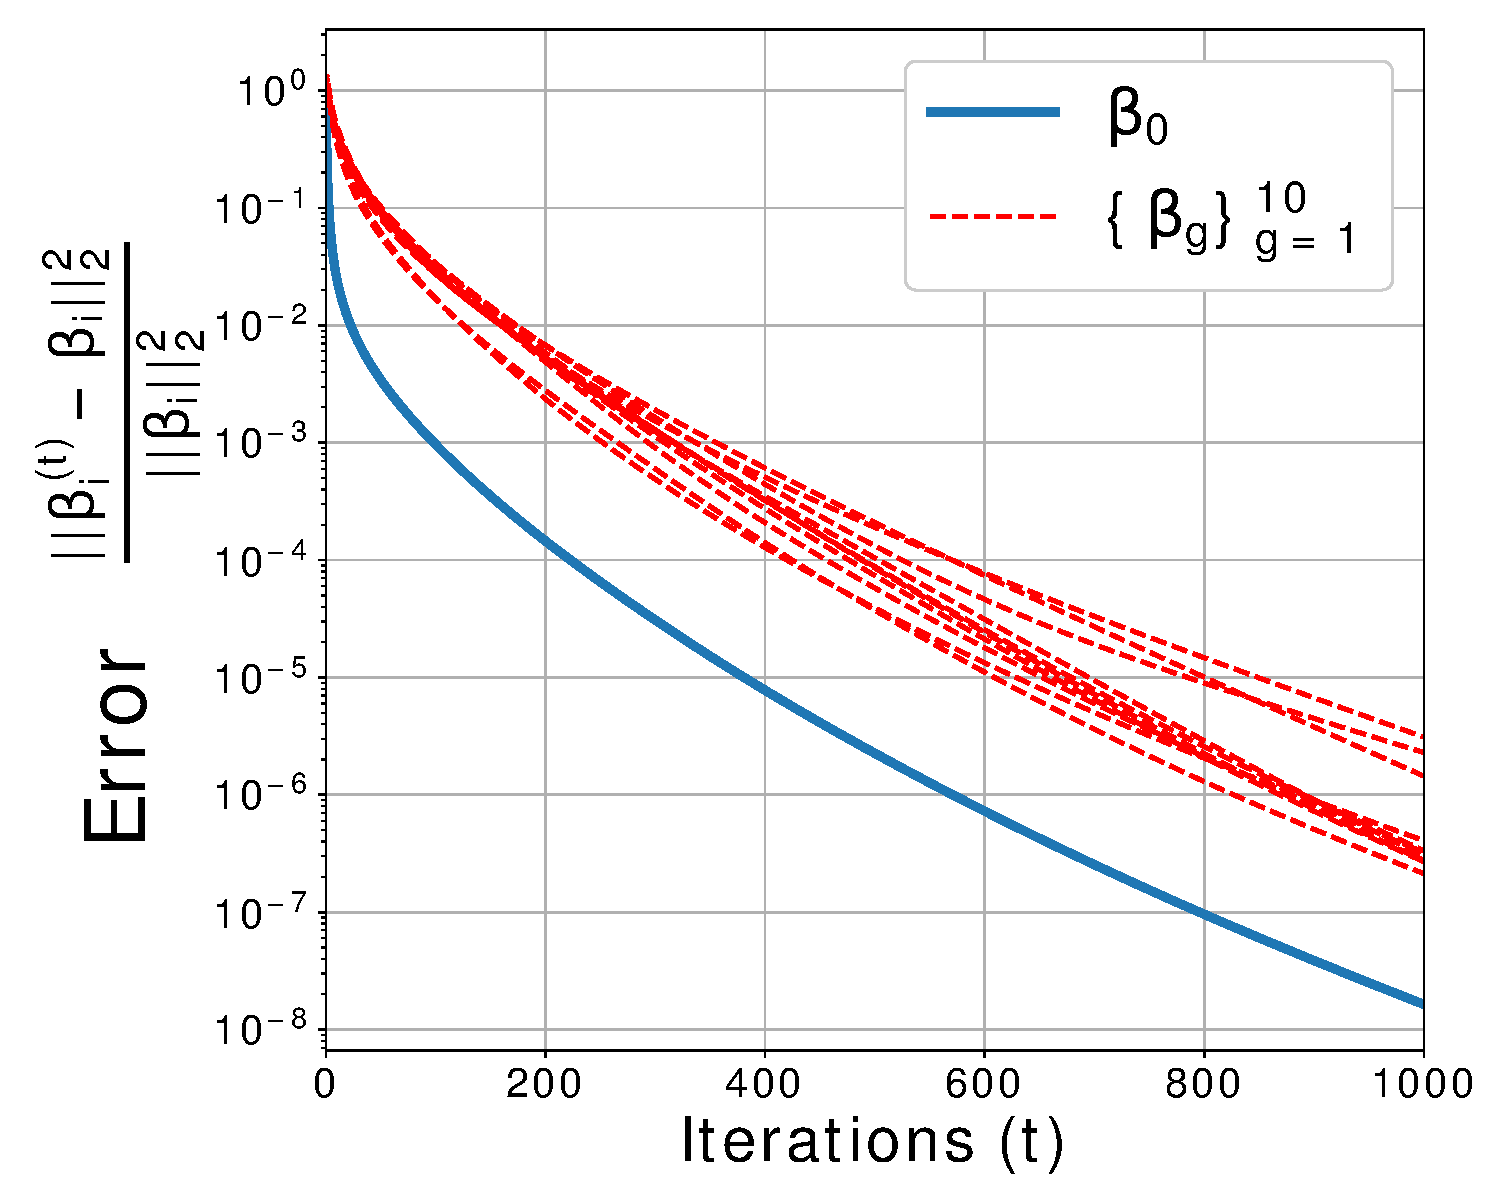
\includegraphics[width=\textwidth]{./img/betag_converge_G10_p100.pdf}				
		\caption{$n_g = 60$, $\w = 0$}\label{fig syn1a}
	\end{subfigure} ~
	\begin{subfigure}[b]{0.2175\textwidth}
		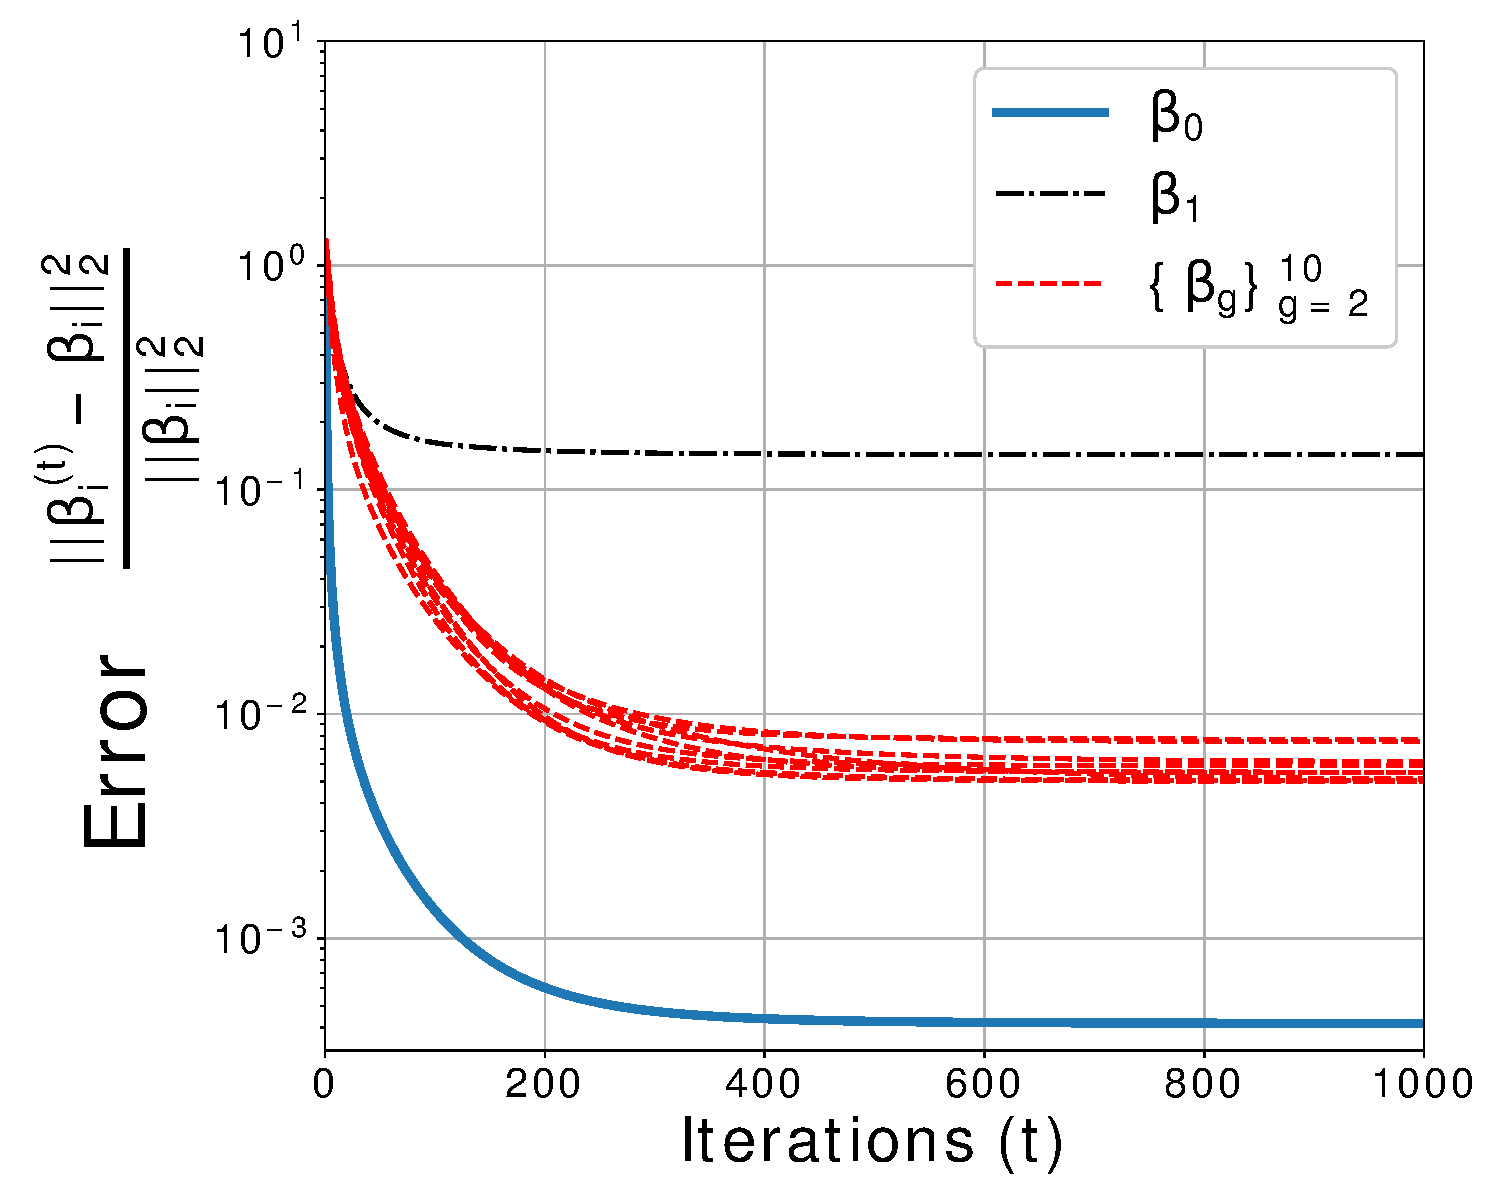
\includegraphics[width=\textwidth]{./img/betag_converge_noise_G10_p100.pdf}				
		\caption{$n_g = 60$, $\w_1 \neq 0$}\label{fig syn1b}
	\end{subfigure}
	%			\label{fig syn1}
	\begin{subfigure}[b]{0.2175\textwidth}
		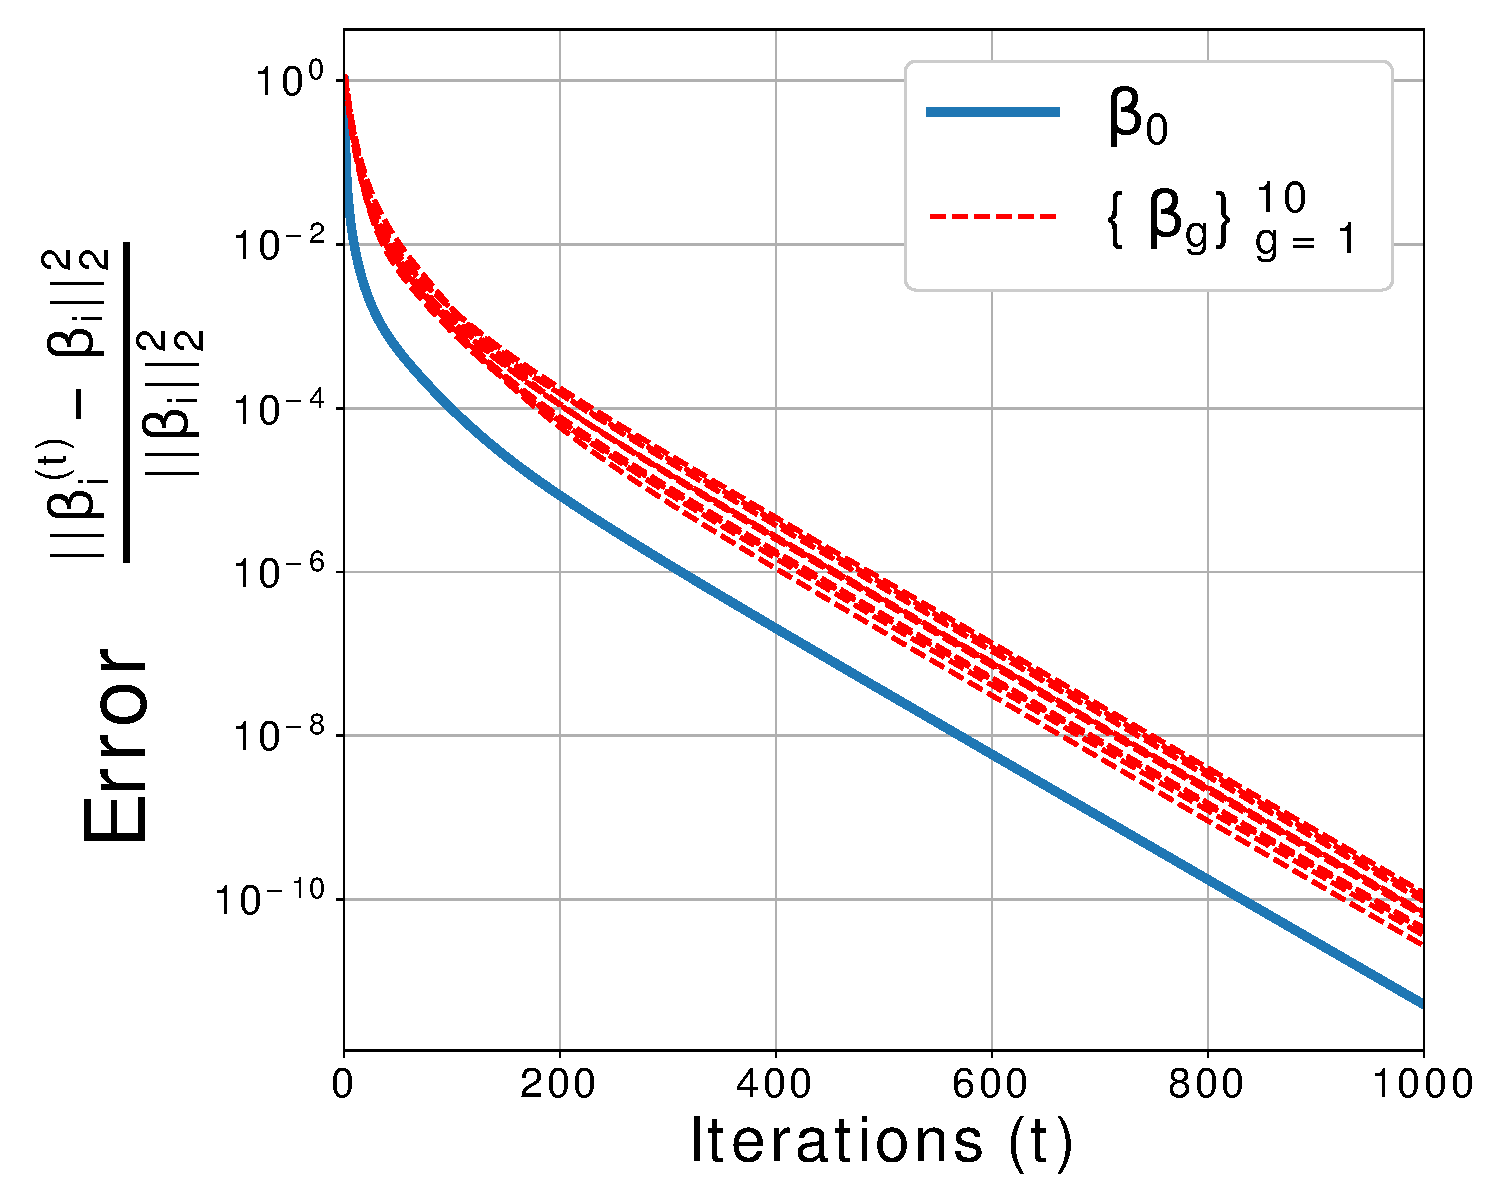
\includegraphics[width=\textwidth]{./img/betag_converge_G10_p100_fast.pdf}
		\caption{$n_g = 150$, $\w = 0$} \label{fig syn2a}
	\end{subfigure} ~
	\begin{subfigure}[b]{0.2175\textwidth}
		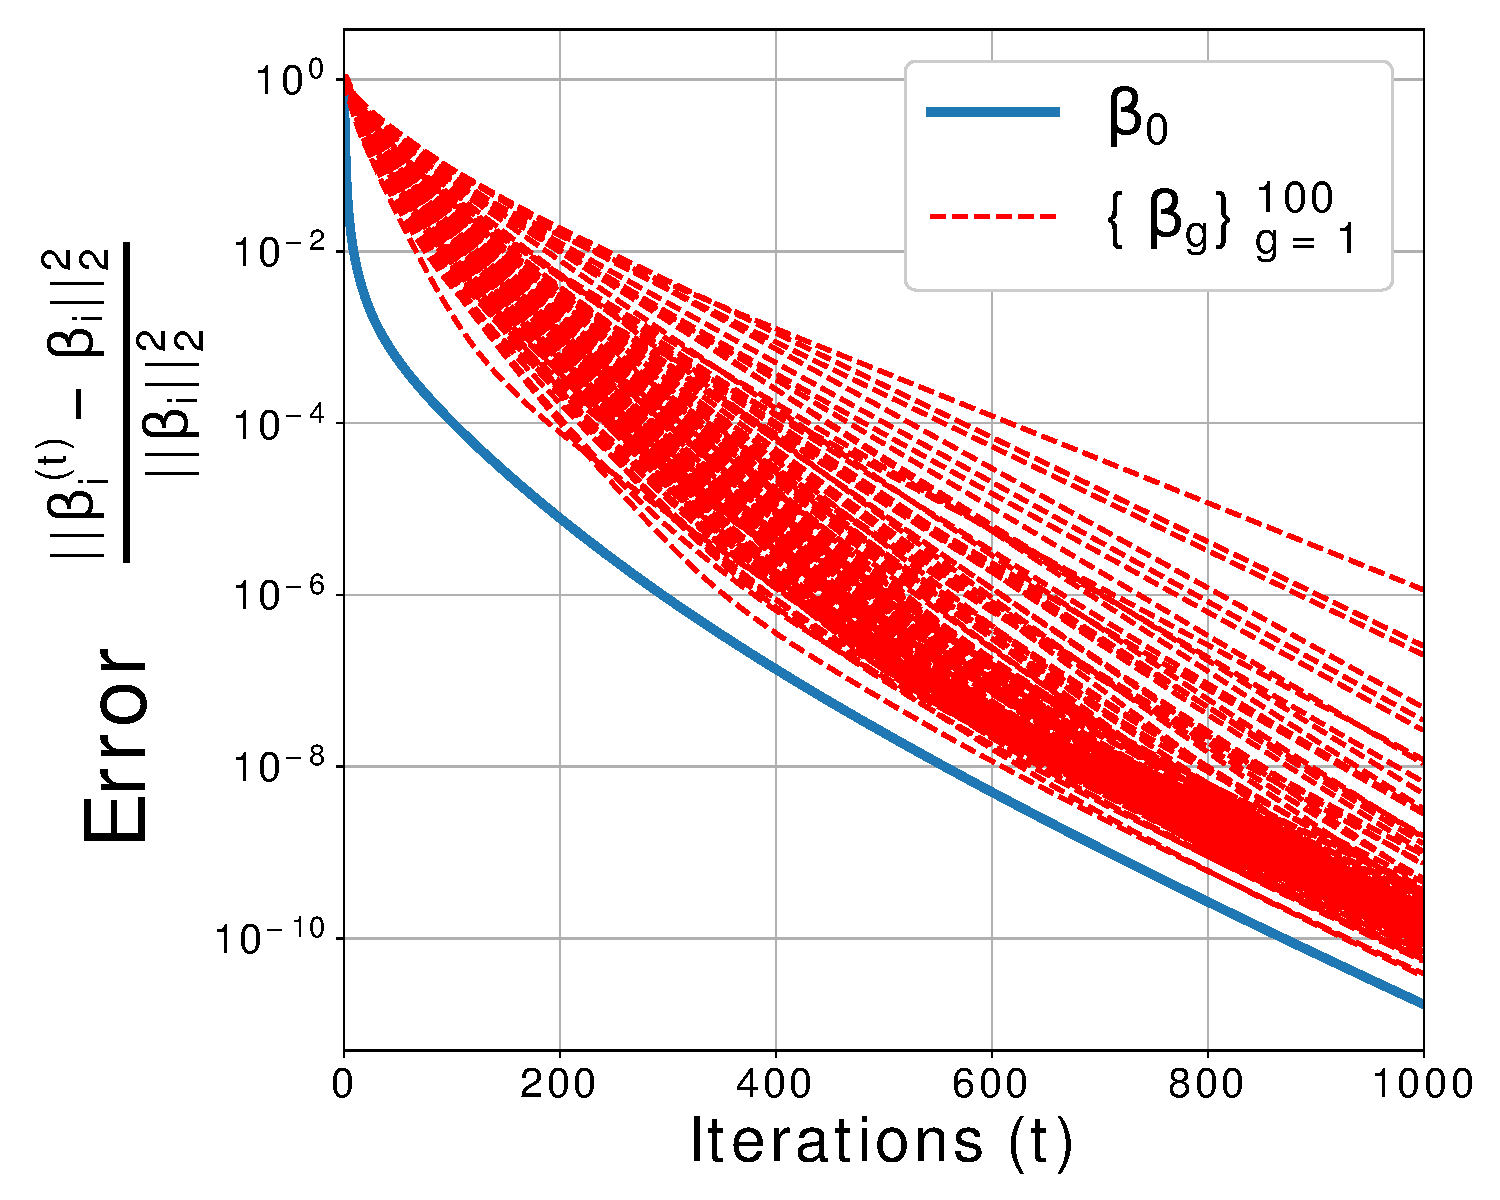
\includegraphics[width=\textwidth]{./img/betag_converge_G100_p1000_shrink.pdf}
		\caption{$n_g = 150$, $\w = 0$}\label{fig syn2b}
	\end{subfigure}
	\squeezeup
	\caption{In (a), (b), and (c)  experiments $p = 100$, $G = 10$, $\forall g \in [G]: s_g = 10$, and $s_0 = p$. For (d) $p = 1000$, $G = 100$, $\forall g \in [G]: s_g = 10$, and $s_0 = 100$. (a) Noiseless fast convergence. (b) Noise on the first group does not impact other groups as much. (c) Increasing sample size improves rate of convergence. (d) \dc\ convergences fast even with a large number of groups $G=100$.}
	\label{fig syn12}
\end{figure}
\section{Experiments on Synthetic Data}
\label{sec:expds}
We considered sparsity based simulations with varying $G$ and sparsity levels. In our first set of simulations, we set $p=100$, $G=10$ and sparsity of the individual parameters to be $s=10$. We generated a dense $\bbeta_0$ with $\|\bbeta_0\|=p$ and did not impose any constraint. Iterates $\{\bbeta^{(t)}_g\}_{g=1}^G$ are obtained by projection onto the $\ell_1$ ball $\|\bbeta_g\|_1$. Nonzero entries of $\bbeta_g$ are generated with ${\cal{N}}(0,1)$ and nonzero supports are picked uniformly at random. Inspired from our theoretical step size choices, in all experiments, we used simplified learning rates of $\frac{1}{n}$ for $\bbeta_0$ and $\frac{1}{\sqrt{nn_g}}$ for $\bbeta_g$, $g \in [G]$. Observe that, cones of the individual parameters intersect with that of $\bbeta_0$ hence this setup actually violates \ds\ (which requires an arbitrarily small constant fraction of groups to be non-intersecting). Our intuition is that the individual parameters are mostly incoherent with each other and the existence of a nonzero perturbation over $\bbeta_g$'s that keeps all measurements intact is unlikely. Remarkably, experimental results still show successful learning of all parameters from small amount of samples. We picked $n_g=60$ for each group. Hence, in total, we have $11p=1100$ unknowns, $200=G\times 10+100$ degrees of freedom and $G\times 60=600$ samples. In all figures, we study the normalized squared error $\frac{\|\bbeta^{(t)}_g-\bbeta_g\|_2^2}{\|\bbeta_g\|_2^2}$ and average $10$ independent realization for each curve. \cref{fig syn1a} shows the estimation performance as a function of iteration number $t$. While each group might behave slightly different, we do observe that all parameters are linear converging to ground truth.% is evident from the linear slope of the $y$-axis.
	
In \cref{fig syn1b}, we test the noise robustness of our algorithm. We add a ${\cal{N}}(0,1)$ noise to the $n_1=60$ measurements of the first group \emph{only}. The other groups are left untouched. While all parameters suffer nonzero estimation error, we observe that, the global parameter $\bbeta_0$ and noise-free groups $\{\bbeta_g\}_{g=2}^G$ have substantially less estimation error. This implies that noise in one group mostly affects itself rather than the global estimation. In \cref{fig syn2a}, we increased the sample size to $n_g=150$ per group. We observe that, in comparison to \cref{fig syn1a}, rate of convergence receives a boost from the additional samples as predicted by our theory.
	
	
Finally, \cref{fig syn2b} considers a very high-dimensional problem where $p=1000$, $G=100$, individual parameters are $10$ sparse, $\bbeta_0$ is $100$ sparse and $n_g=150$. The total degrees of freedom is $1100$, number of unknowns are $101000$ and total number of datapoints are $150\times 100=15000$. While individual parameters have substantial variation in terms of convergence rate, at the end of $1000$ iteration, all parameters have relative reconstruction error below $10^{-6}$.
%	\begin{figure}[t!]
%		\begin{subfigure}[b]{0.5\textwidth}
%			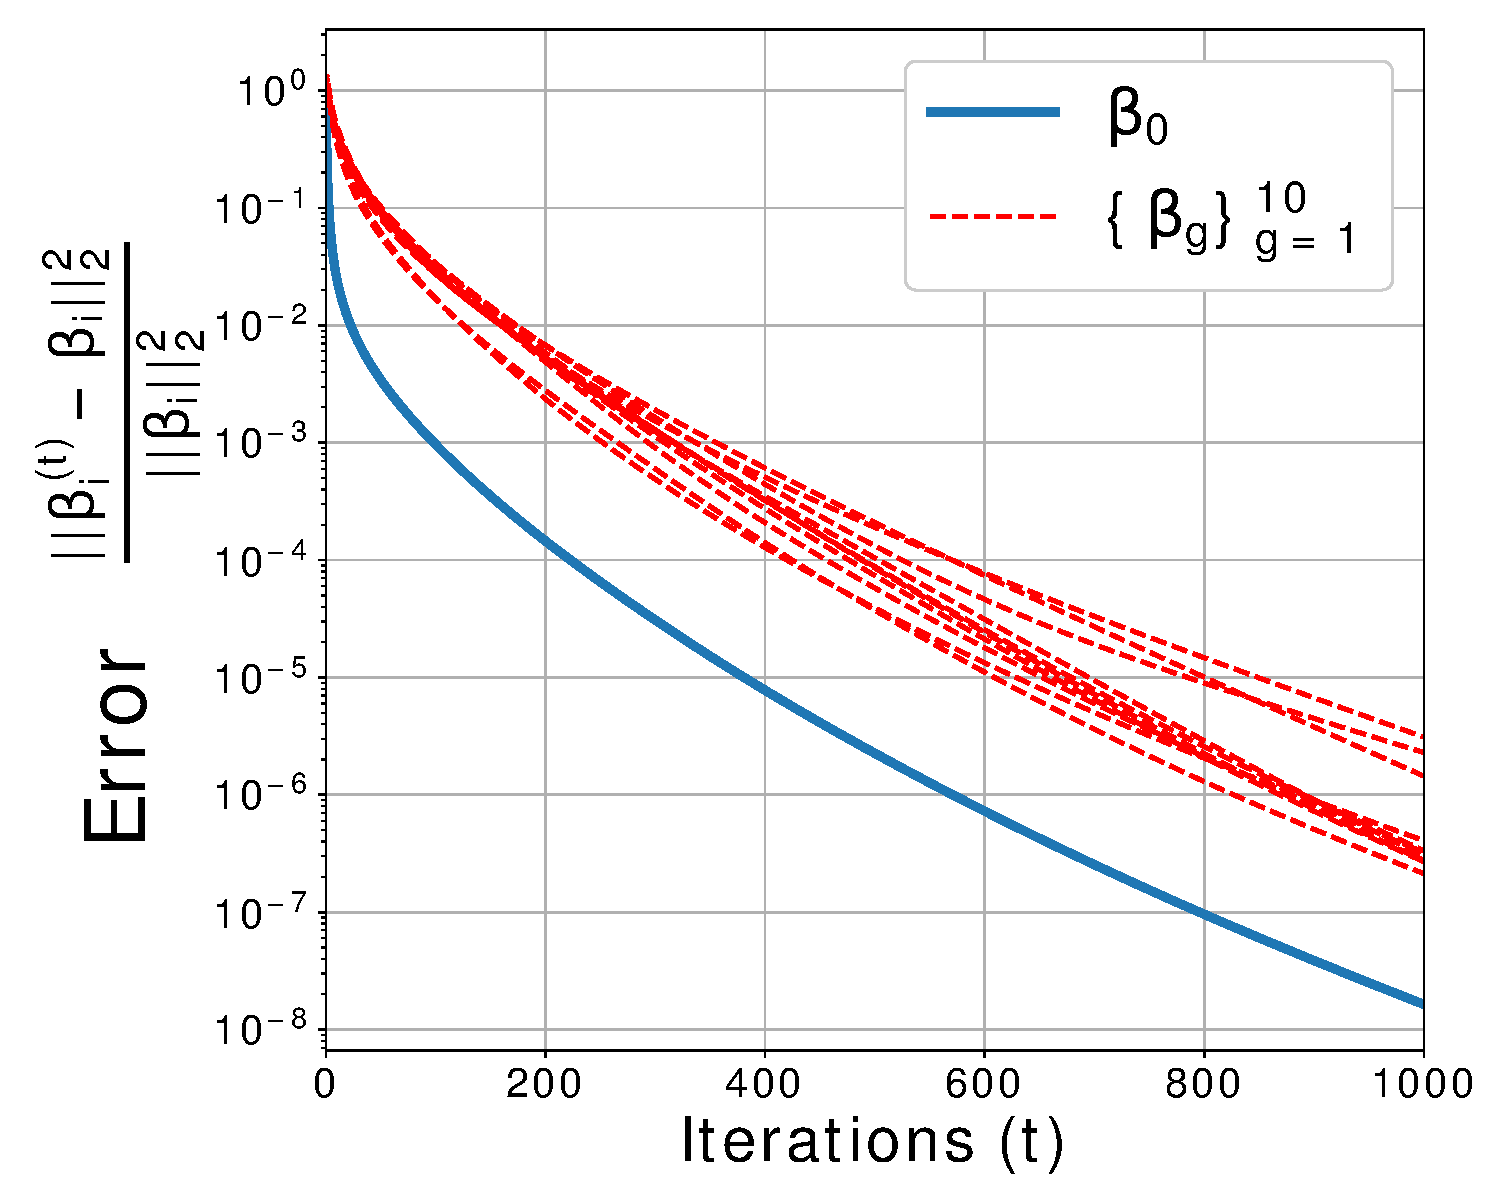
\includegraphics[width=\textwidth]{img/betag_converge_G10_p100.eps}
%			
%			\caption{}\label{fig syn1a}
%		\end{subfigure} ~
%		\begin{subfigure}[b]{0.5\textwidth}
%			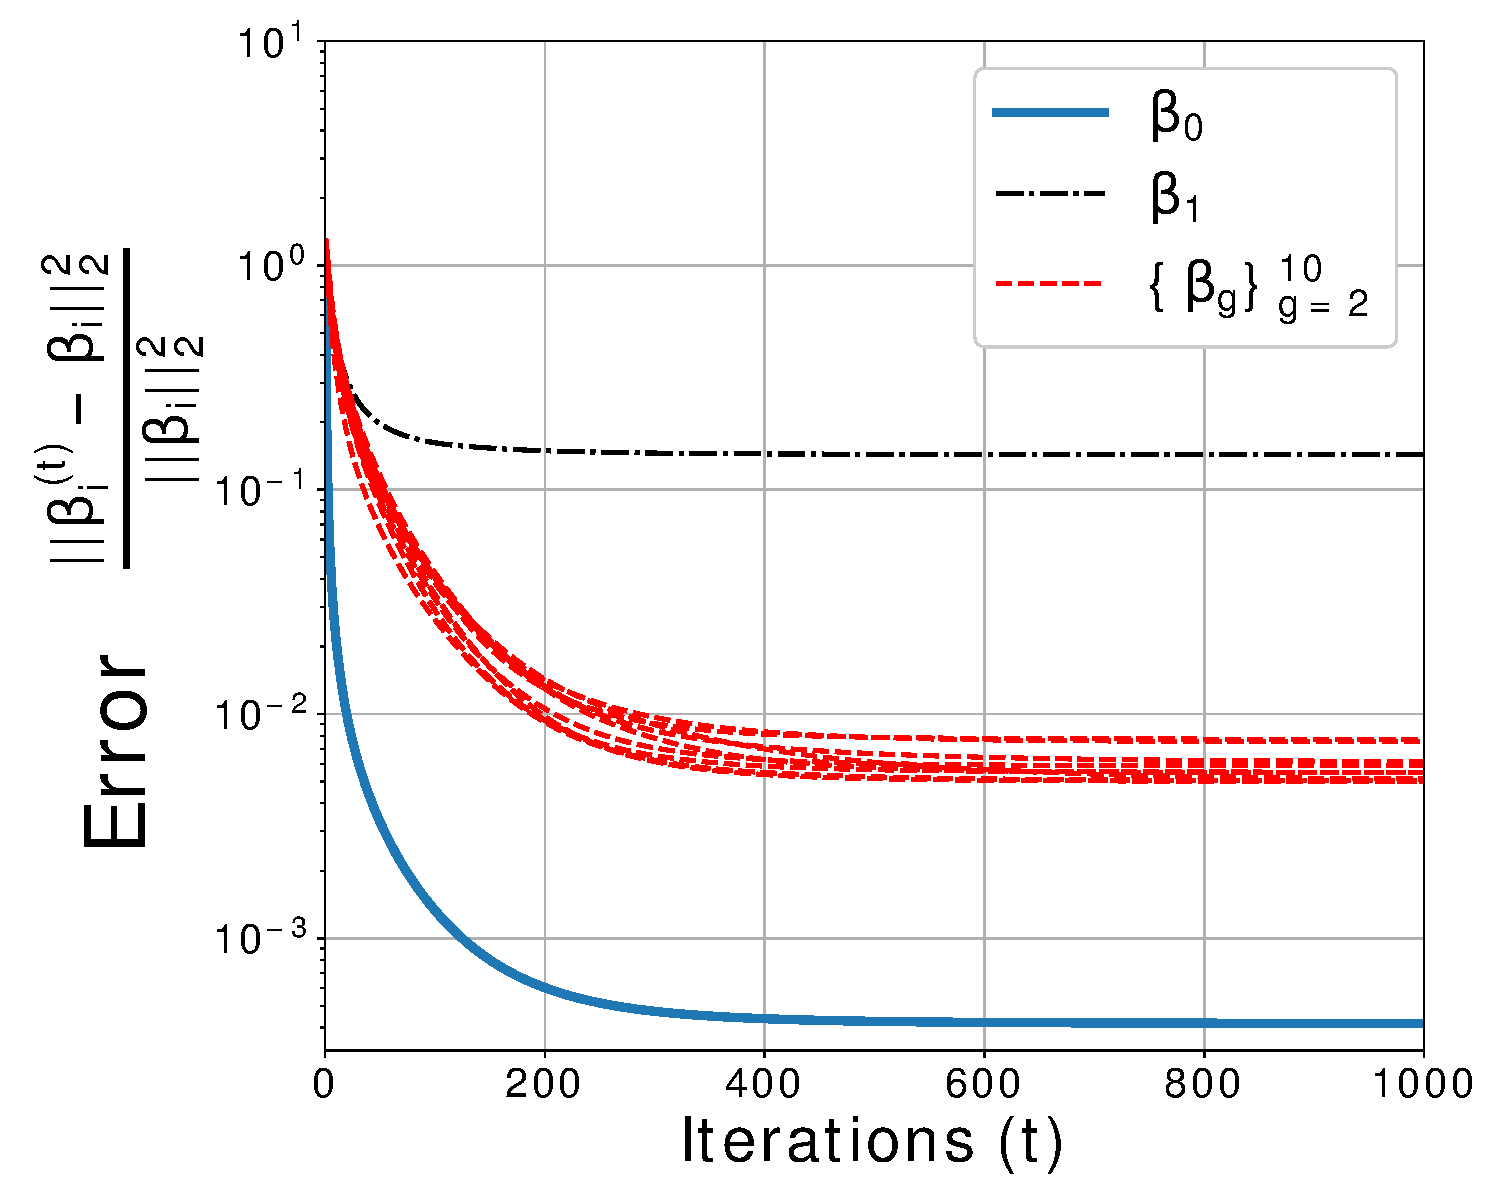
\includegraphics[width=\textwidth]{img/betag_converge_noise_G10_p100.eps}
%			
%			\caption{}\label{fig syn1b}
%		\end{subfigure}
%		\caption{a) Noiseless fast convergence. b) Noise on the first group does not impact other groups as much.}
%		\label{fig syn1}
%	\end{figure}
%	
%	\begin{figure}[t!]
%		\begin{subfigure}[b]{0.5\textwidth}
%			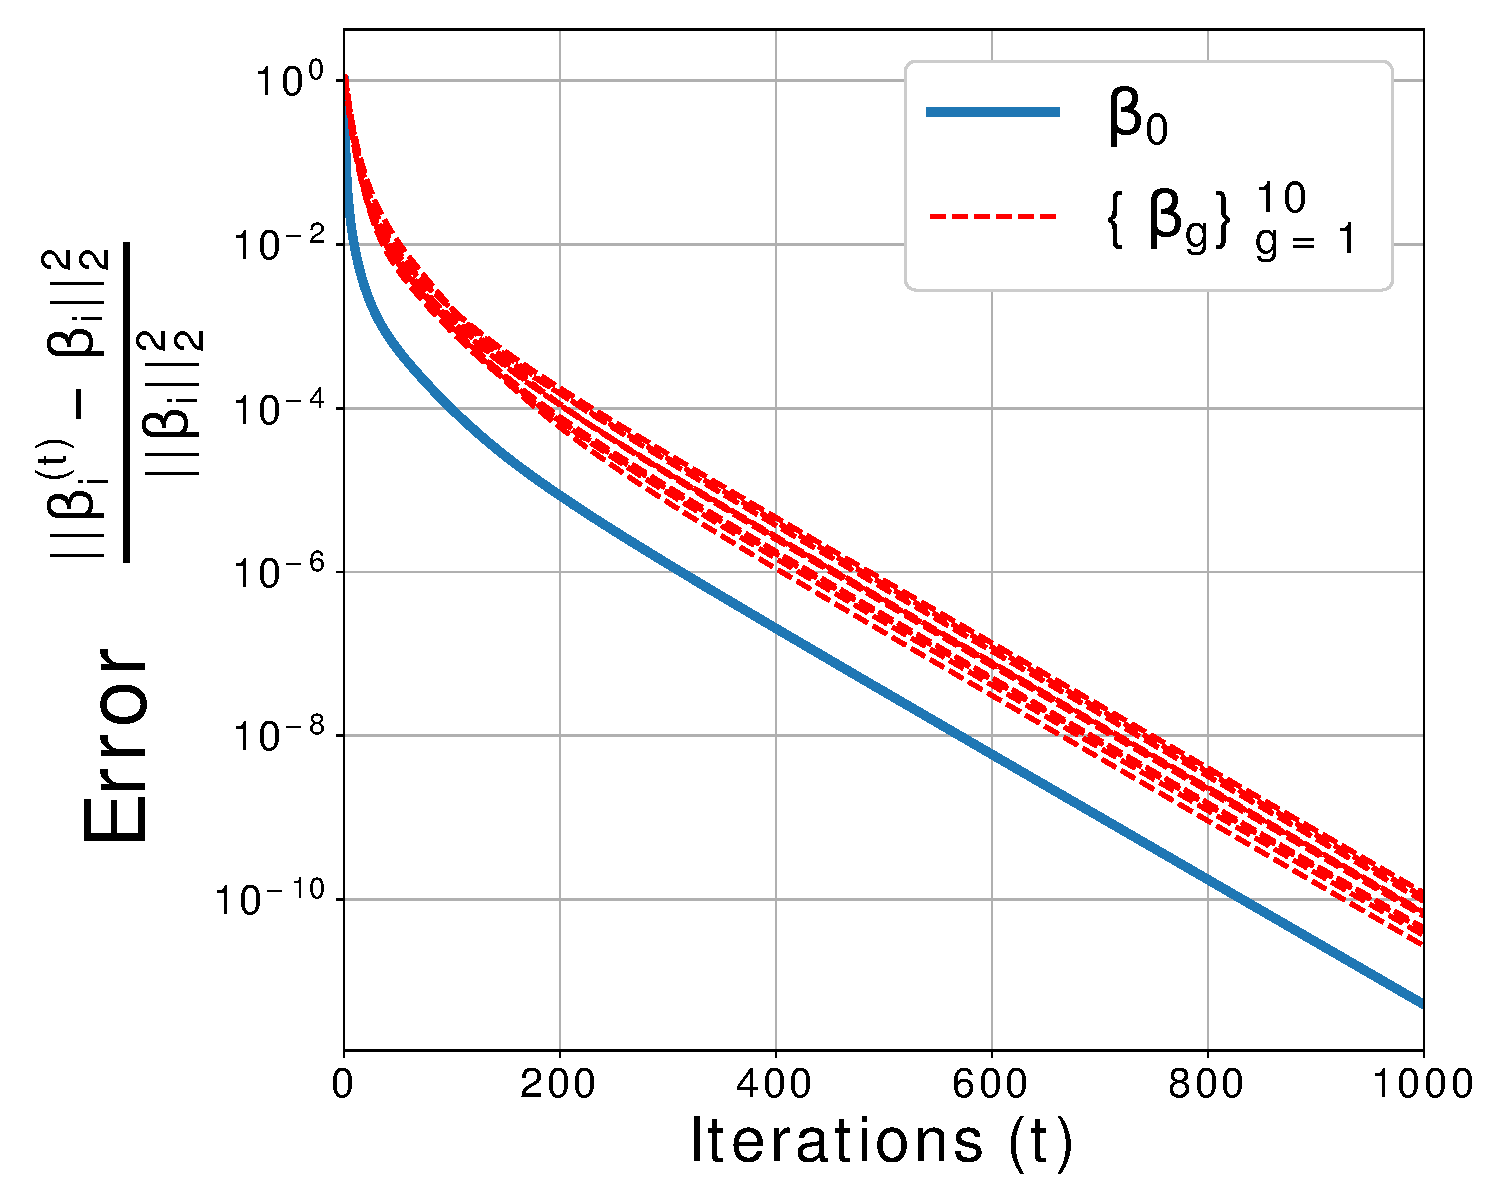
\includegraphics[width=\textwidth]{img/betag_converge_G10_p100_fast.eps}
%			
%			\caption{} \label{fig syn2a}
%		\end{subfigure} ~
%		\begin{subfigure}[b]{0.5\textwidth}
%			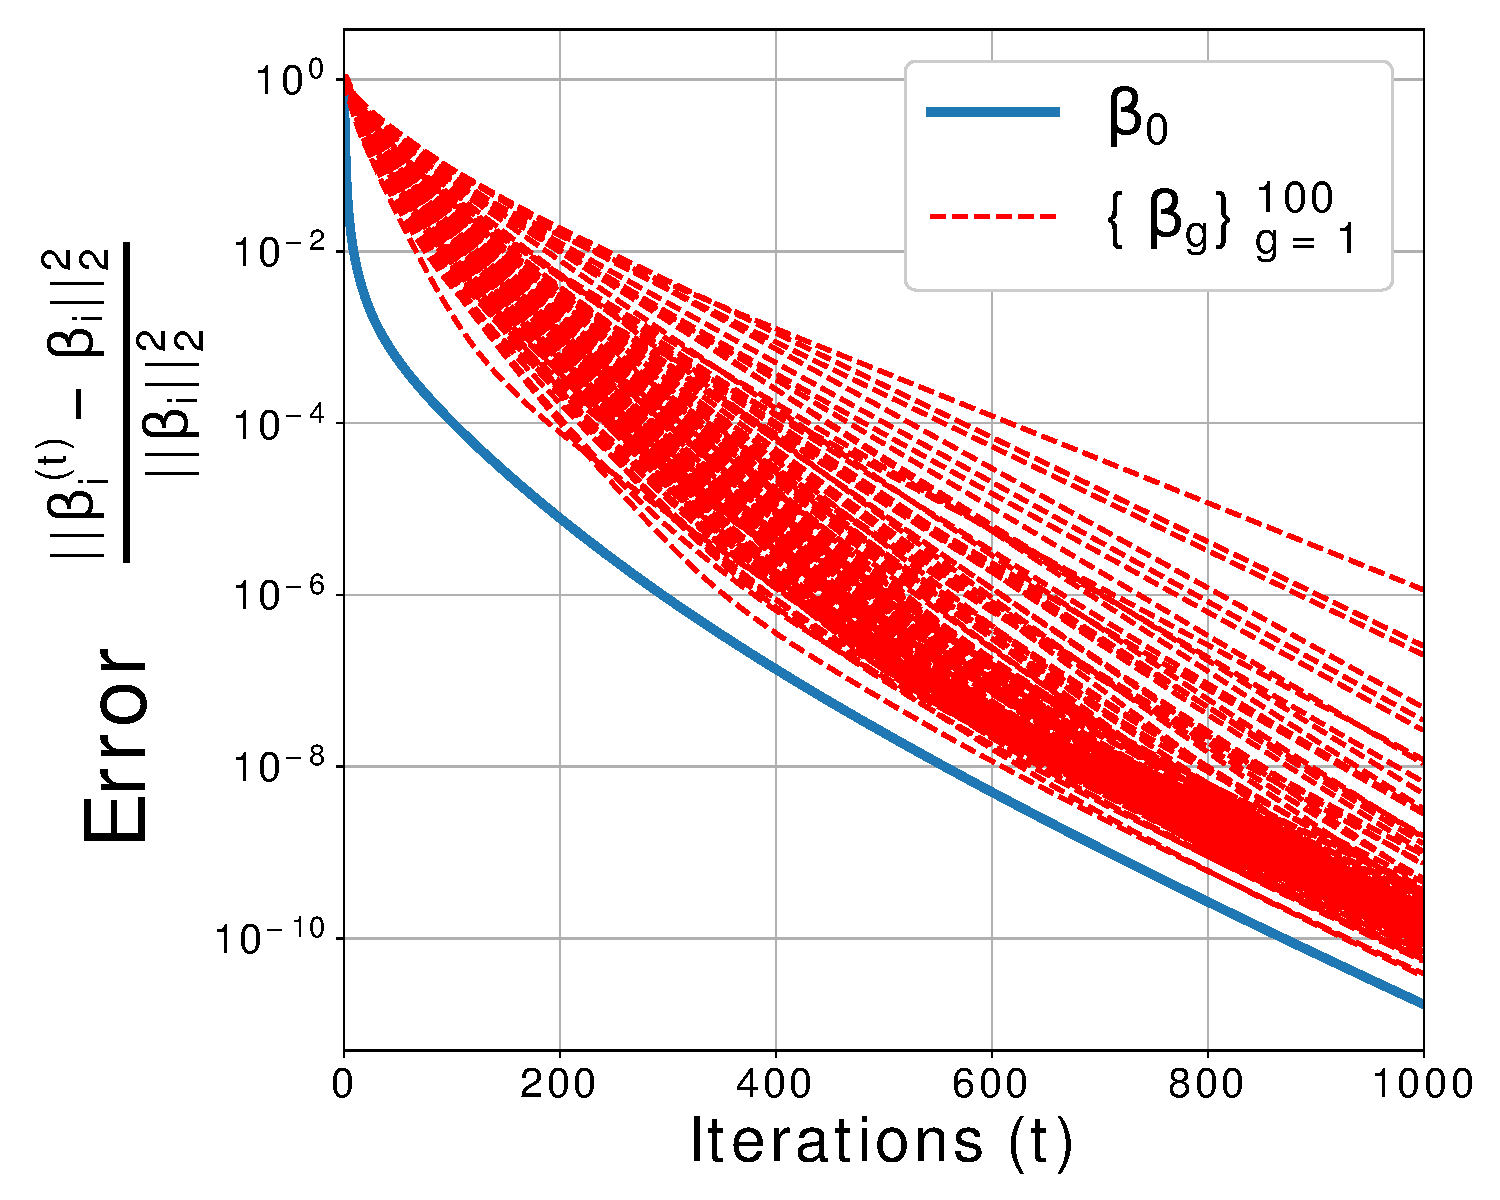
\includegraphics[width=\textwidth]{img/betag_converge_G100_p1000_shrink}
%			
%			\caption{}\label{fig syn2b}
%		\end{subfigure}
%		\caption{a) Increasing sample size improves rate of convergence. b) Our algorithm convergences fast even with a large number of groups $G=100$.}
%		\label{fig syn2}
%	\end{figure}



%%%%%%%%%%%%% Amir's exp commented for now
%In this section we supplement our theoretical results with a simple synthetic experiment. 
%We focus on the case of two groups, i.e., $G = 2$. 
%The dimension $p = 1000$ and the structure is sparsity induced by $l_1$-norm. 
%The parameters $\bbeta _0^*$, $\bbeta _1^*$, and $\bbeta _2^*$ are 20, 10, and 5-sparse respectively. 
%The sparsity pattern is as follows:$\bbeta _0^* = (\underbrace{1, \dots, 1}_{1-20}, 0, \dots)$,$\bbeta _1^* = (\dots, 0, \underbrace{2, \dots, 2}_{51-60}, 0, \dots)$, and $\bbeta _2^* = (\dots, 0, \underbrace{-2, \dots, -2}_{96-100}, 0, \dots)$. 
%
%For the distribution of input and noise we have $\x_{gi} \sim N(0, \sigma_x^2 \I)$ and $\omega_{gi} \sim N(0, \sigma_w^2)$ with $\sigma_x^2 = .3$ and  $\sigma_w^2 = .1$.
%We use the SPGD method (Algorithm \cref{alg2}) to solve the optimization problem \cref{eq:compact}. 
%The projection to the $l_1$ ball can be efficiently performed by the method proposed in \cite{dssc08}. 
%
%While changing $n$ in the experiments, we keep the ratio $\frac{n_1}{n_2} = \frac{2}{3}$ fixed. 
%Figures \cref{fig:individual1} and \cref{fig:individual2} show the per-group error for different sample size which follows $1/\sqrt{n_g}$ decay.
%Finally, Figure \cref{fig:common} shows the decay of the error as sample size increases for the common component recovery and the error for summation of the form \cref{eq:errorsum}.
%As expected errors decay as $1/\sqrt{n}$.
%
%\begin{figure}
%	\centering
%	\subcaptionbox{
%		Individual parameter one.
%		\label{fig:individual1}
%	}{\includegraphics[width=0.3 \textwidth]{./img/synthbeta1}}~
%	\subcaptionbox{
%		Individual parameter two.
%		\label{fig:individual2}
%	}{\includegraphics[width=0.3 \textwidth,]{./img/synthbeta2}}
%	\subcaptionbox{
%		Common parameter.
%	\label{fig:common}
%	}{\includegraphics[width=0.3 \textwidth,]{./img/synthbeta0}}
%	\caption{Estimation error with different sample size. Each point on the diagram is an average over 30 experiments.} %\cref{fig:common} compares the error with the LHS of \cref{eq:errorsum}
%	\label{fig:gasprices}
%\end{figure}



	
	%\section{Conclusion}
We presented an estimator for the joint estimation of common and individual parameters of the data sharing model. 
We showed that the sample complexity for estimation of the shared parameter depends on the total number of sample $n$.
In addition, the shared parameter error rate decays as $1/\sqrt{n}$. 
These results indicate that our estimator benefits from the pooled data in estimating the common parameters. 
Both sample complexity and upper bound of error depend on the \emph{maximum} Gaussian width among the spherical caps induced by the error cones of all parameters.
We provided a projected gradient descent algorithm for estimation of the parameters and analyzed its convergence rate and showed geometric convergence for a carefully selected step size. Finally, we complemented the theoretical results presented with simulation results.

	\pagebreak
	\bibliographystyle{icml2019}
	\bibliography{nips18}
	
	
	%%%%%%%%%%%%%%%%%%%%%%%%%%%%%%%%%%%%%%%%%%%%%%%%%%%%%%%%%%%%%%%%%%%%%%%%%%%%%%%
	%%%%%%%%%%%%%%%%%%%%%%%%%%%%%%%%%%%%%%%%%%%%%%%%%%%%%%%%%%%%%%%%%%%%%%%%%%%%%%%
	% DELETE THIS PART. DO NOT PLACE CONTENT AFTER THE REFERENCES!
	%%%%%%%%%%%%%%%%%%%%%%%%%%%%%%%%%%%%%%%%%%%%%%%%%%%%%%%%%%%%%%%%%%%%%%%%%%%%%%%
	%%%%%%%%%%%%%%%%%%%%%%%%%%%%%%%%%%%%%%%%%%%%%%%%%%%%%%%%%%%%%%%%%%%%%%%%%%%%%%%
	
	\appendix
	
	\newpage 
\onecolumn
\section{Proofs of Theorems}
\label{sec:dsproofs}
In this Section we present detail proof for each theorem and proposition. To avoid cluttering, during our proofs, we state some needed results as lemmas and provide their proof in the next Section \ref{sec:lemmas}. 

\subsection{Proof of Theorem \ref{theo:deter}}
\begin{proof}
	Starting from the optimality inequality, for the lower bound with the set $\cH$ we get:
	\be 
	\label{eq:tre} 
	\frac{1}{n}\norm{\X \ddelta}{2}^2 &\geq& \frac{1}{n} \inf_{\u \in \cH} \norm{\X \u}{2}^2  \left(\sum_{g=0}^{G} {\frac{n_g}{n}} \norm{\ddelta_g}{2} \right)^2 \\ \nr
	&\geq& \kappa  \left(\sum_{g=0}^{G} {\frac{n_g}{n}} \norm{\ddelta_g}{2} \right)^2  \nr
	\\ \nr 
	&\geq& \kappa  \left(\min_{g \in [G] } \frac{n_g}{n}\right) \left(\sum_{g=0}^{G} \sqrt{\frac{n_g}{n}} \norm{\ddelta_g}{2} \right)^2  
	\ee 
	where $0 < \kappa \leq \frac{1}{n}  \inf_{\u \in \cH} \norm{\X \u}{2}^2 $ is known as Restricted Eigenvalue (RE) condition. 
	The upper bound will factorize as:
	\be 
	\label{eq:tub}
	\frac{2}{n}\oomega^T \X\ddelta &\leq& \frac{2}{n} \sup_{\u \in \bcH} \oomega^T \X \u \left(\sum_{g=0}^{G} \sqrt{\frac{n_g}{n}} \norm{\ddelta_g}{2} \right) , \quad \u \in \cH \\ \nr 
	\ee 
	Putting together inequalities \eqref{eq:tre} and \eqref{eq:tub} completes the proof.% for the set $\cH$. 
%	
%	Now in the lower bound we use the set $\bcH$ and for the upper bound we keep the set $\cH$. 
%	We have:
%	\be 
%	\nr 
%	\kappa  \left(\sum_{g=0}^{G} \beta_g \norm{\ddelta_g}{2} \right)^2  \leq \frac{2}{n} \sup_{\u \in \cH} \oomega^T \X \u \left(\sum_{g=0}^{G} \sqrt{\frac{n_g}{n}} \norm{\ddelta_g}{2} \right),
%	\ee 
%	where $\beta_g = \frac{n_g}{n}$.
%	Noting that $\left(\sum_{g=0}^{G} \sqrt{\frac{n_g}{n}} \norm{\ddelta_g}{2} \right) / \left(\sum_{g=0}^{G} \frac{n_g}{n} \norm{\ddelta_g}{2} \right) \leq G$ complete the proof for the set $\bcH$. 
%	\be 
%	\sum_{g=0}^{G} {\frac{n_g}{n}} \norm{\ddelta_g}{2} \leq \frac{2}{n\kappa} \sup_{\u \in \bcH} \oomega^T \X \u \frac{\left(\sum_{g=0}^{G} \sqrt{\frac{n_g}{n}} \norm{\ddelta_g}{2} \right) }{\left(\sum_{g=0}^{G} {\frac{n_g}{n}} \norm{\ddelta_g}{2} \right) }
%	\ee 
\end{proof}

\subsection{Proof of Proposition \ref{prop:super}}
\begin{proof}
	Consider only one group for regression in isolation. 
	Note that $\y_g = \X_g (\bbeta _g^* + \bbeta _0^*) + \oomega_g$ is a superposition model and as shown in \cite{guba16} the sample complexity required for the RE condition and subsequently recovering $\bbeta _0^*$ and $\bbeta _g^*$ is $n_g  \geq c(\max_{g \in [G]}\omega(\cA_g) + \sqrt{\log 2})^2$.
\end{proof} 

%\subsection{Proof of Lemma \ref{lemm:secTerm}}
%\begin{definition}[Data sharing incoherence condition]  \label{incodef}For some scalars $0\leq \ratio\leq 1$ and $\lamin>0$ the following holds. There exists a set $\Gin\subset \Gsm$ such that
%	\begin{itemize}
%		\item $\sum_{i\in \Gin} n_i\geq \lceil \ratio n\rceil$.
%		\item For all $i\in \Gin$, and for all $\ddelta_i\in\cC_i,\ddelta_0\in\cC_0$, we have that
%		\[
%		\tn{\ddelta_i+\ddelta_0}\geq \lamin (\tn{\ddelta_0}+\tn{\ddelta_i}).
%		\]
%	\end{itemize}
%	Observe that $0\leq \lamin,\ratio\leq 1$ by definition.
%\end{definition}

%\begin{lemma} \label{incolem} Suppose Definition \ref{incodef} holds. Then, for any $\ddelta_i\in \cC_i$ for $0\leq i\leq G$, we have that
%\[
%\sum_{i=1}^G \tn{\ddelta_0+\ddelta_i}\geq\frac{\ratio\lamin}{3} (G\tn{\ddelta_0}+\sum_{i=1}^G\tn{\ddelta_i}).
%\]
%\end{lemma}
%\begin{proof} We split $\Gsm-\Gin$ into two groups $G_1,G_2$. $G_1$ consists of $\ddelta_i$'s with $\tn{\ddelta_i}\geq 2\tn{\ddelta_0}$ and $G_2=\Gsm-\Gin-G_1$. We use the bounds
%\[
%\tn{\ddelta_0+\ddelta_i}\geq \begin{cases}\tn{\ddelta_i}/2~\text{if}~i\in G_1\\0~\text{if}~i\in G_2\\\lamin(\tn{\ddelta_i}+\tn{\ddelta_0})~\text{if}~i\in \Gin\end{cases}
%\]
%This implies
%\[
%\sum_{i=1}^G \tn{\ddelta_0+\ddelta_i}\geq \sum_{i\in G_1}\frac{1}{2}\tn{\ddelta_i}+\lamin\sum_{i\in \Gin} (\tn{\ddelta_i}+\tn{\ddelta_0}).
%\]
%We know that over $G_2$, $\tn{\ddelta_i}\leq 2\tn{\ddelta_0}$ which implies $\sum_{i\in G_2}\tn{\ddelta_i}\leq 2|G_2|\tn{\ddelta_0}\leq 2G\tn{\ddelta_0}$. Set $\rinc=\min\{1/2,\lamin\ratio/3\}=\lamin\ratio/3$. Let $S_j=\sum_{i\in G_j}\tn{\ddelta_i}$ for $j=1,2,\Ic$. Using $1/2\geq \rinc$ and $\lamin\geq \rinc$, we write
%\begin{align}
%\sum_{i=1}^G \tn{\ddelta_0+\ddelta_i}&\geq \rinc S_1+\lamin\sum_{i\in \Gin} (\tn{\ddelta_i}+\tn{\ddelta_0})\\
%&\geq \rinc S_1+\rinc S_2-2\rinc G\tn{\ddelta_0}+|\Gin|\lamin \tn{\ddelta_0}+\lamin S_{\Ic}\\
%&\geq \rinc (S_1+S_2+S_3)+ (|\Gin|\lamin-2\rinc G)\tn{\ddelta_0}.
%\end{align}
%Now, observe that, by Assumption \ref{incodef}, $|\Gin|\geq \ratio |G|$ which implies 
%\[
%|\Gin|\lamin-2\rinc G\geq (\ratio\lamin -2\rinc)|G|\geq \rinc |G|.
%\]
%Combining all, we obtain
%\[
%\sum_{i=1}^G \tn{\ddelta_0+\ddelta_i}\geq \rinc(|G|\tn{\ddelta_0}+\sum_{i=1}^G \tn{\ddelta_i}).
%\]
%\end{proof}



%\begin{proof}
%	\be 
%	\nr
%	\inf_{\ddelta_0 \in \cC_0, \ddelta_g \in \cC_g} Q_{2\lambda_g \xi_g}(\ddelta_{0g})
%	&=& \inf_{\ddelta_0 \in \cC_0, \ddelta_g \in \cC_g} \pr(|\langle \x, \ddelta_{0} + \ddelta_{g} \rangle| \geq 2\lambda_g \xi_g)
%	\\ \nr 
%	&=& \inf_{\ddelta_0 \in \cC_0, \ddelta_g \in \cC_g} \pr(\norm{\ddelta_{0} + \ddelta_{g}}{2} |\langle \x, \frac{\ddelta_{0} + \ddelta_{g}}{\norm{\ddelta_{0} + \ddelta_{g}}{2}} \rangle| \geq 2\lambda_g \xi_g)
%	\\ \nr 
%	\text{(Individual SC conditions)}  &\geq& \inf_{\ddelta_0 \in \cC_0, \ddelta_g \in \cC_g} \pr(\lambda_g (\norm{\ddelta_{0}}{2} + \norm{\ddelta_{g}}{2}) |\langle \x, \frac{\ddelta_{0} + \ddelta_{g}}{\norm{\ddelta_{0} + \ddelta_{g}}{2}} \rangle| \geq 2\lambda_g \xi_g)
%	\\ \nr 
%	&\geq& \inf_{\ddelta_0 \in \cC_0, \ddelta_g \in \cC_g} \pr((\norm{\ddelta_{0}}{2} + \sqrt{\frac{n_g}{n}} \norm{\ddelta_{g}}{2}) |\langle \x, \frac{\ddelta_{0} + \ddelta_{g}}{\norm{\ddelta_{0} + \ddelta_{g}}{2}} \rangle| \geq 2 \xi_g)
%	\\ \nr
%	\text{(i)} &\geq& \inf_{\u \in \cA_{0g}} \pr\left(|\langle \x, \u \rangle| \geq 2 \xi\right)
%	\\ \nr 
%	&=& \inf_{\u\in \cA_{0g}} Q_{2\xi}(\u; \cA_{0g}) 
%	\ee 
%	where in (i) we set $\xi_g = \xi \min_{\ddelta_0 \in \cC_0, \ddelta_g \in \cC_g}  (\norm{\ddelta_0}{2} + \sqrt{\frac{n_g}{n}} \norm{\ddelta_g}{2})$ for some $\xi > 0$	and $\cA_{0g} = \{\ddelta_0 + \ddelta_g | \ddelta_0 \in \cC_0, \ddelta_g \in \cC_g, \norm{\ddelta_0 + \ddelta_g}{2} = 1\}$.
%	Note that our choice of $\xi_g$ will not affect the upper bound of the second term $t_2(\X)$ of \eqref{eq:long}, for more on this refer to the proof of Lemma \ref{lemm:secTerm} in Section \ref{sec:proofSecTerm}.
%\end{proof}

%\subsection{Proof of Lemma \ref{lemm:secTerm}}

%
\subsection{Proof of Theorem \ref{theo:re}}

Let's simplify the LHS of the RE condition:% \eqref{eq:recond}: 
\be 
\nr 
\frac{1}{\sqrt{n}} \norm{\X \ddelta}{2} 
%&=& \frac{1}{\sqrt{n}} \normlr{\begin{pmatrix}
%		\X_1 (\ddelta_0 + \ddelta_1) \\
%		\X_2 (\ddelta_0 + \ddelta_2) \\ 
%		\vdots  \\
%		\X_G (\ddelta_0 + \ddelta_G)
%\end{pmatrix}}{2} 
%\\ \nr 
&=& \left(\frac{1}{n} \sum_{g=1}^{G} \sum_{i=1}^{n_g} |\langle \x_{gi}, \ddelta_0 + \ddelta_g \rangle|^2\right)^{\frac{1}{2}}
\\ \nr
%\text{(Lyapunov's Inequality)} 
&\geq& \frac{1}{n} \sum_{g=1}^{G} \sum_{i=1}^{n_g} |\langle \x_{gi}, \ddelta_0 + \ddelta_g \rangle| 
\\ \nr 
&\geq& \frac{1}{{n}} \sum_{g=1}^{G} \xi\norm{\ddelta_0+\ddelta_g}{2}  \sum_{i=1}^{n_g} \indic \left(|\langle \x_{gi}, \ddelta_0 + \ddelta_g \rangle| \geq \xi\norm{\ddelta_0+\ddelta_g}{2}\right),
\ee 
where the first inequality is due to Lyapunov's inequality.
To avoid cluttering we denote $\ddelta_{0g} = \ddelta_0 + \ddelta_g$ where $\ddelta_0 \in \cC_0$ and $\ddelta_g \in \cC_g$.
Now we add and subtract the corresponding per-group marginal tail function, $Q_{\xi_g}(\ddelta_{0g}) = \pr(|\langle \x, , \ddelta_{0g} \rangle| > \xi_g)$ where $\xi_g > 0$. 
Let $\xi_g=\norm{\ddelta_{0g}}{2}\xi$ then the LHS of the RE condition reduces to: 
%Argument $\cH$ emphasizes that $\ddelta_{0g} = \ddelta_{0} + \ddelta_{g}$ has summands from components of $\ddelta = (\ddelta_0^T, \dots, \ddelta_G^T)^T$  where $\ddelta \in \cH$. 
%To simplify the notation, we drop $\cH$ from the marginal tail function and specify it only when it is not from the context:
%{\small
%\be
%\nr 
%&&\frac{1}{\sqrt{n}} \norm{\X \ddelta}{2} %\geq \frac{1}{n} \sum_{g=1}^{G} \lambda_g \xi_g  \sum_{i=1}^{n_g} \indic (|\langle \x_{gi}, \ddelta_{0g} \rangle| \geq \lambda_g \xi_g) 
%%\\ \nr
%\geq \frac{1}{n} \sum_{g=1}^{G} n_g \xi_g  \lambda_g Q_{2\lambda_g \xi_g}(\ddelta_{0g}; \cH) -
%\\ \nr	
%&& \frac{1}{n} \sum_{g=1}^{G} \xi_g  \lambda_g \sum_{i=1}^{n_g} \left[Q_{2\lambda_g \xi_g}(\ddelta_{0g}; \cH)  - \indic (|\langle \x_{gi}, \ddelta_{0g} \rangle| \geq \lambda_g \xi_g)  \right]
%\\ \nr
%\ee
%} 
%\be
%	\label{eq:long}
%	\inf_{\ddelta \in \cH} \frac{1}{\sqrt{n}} \norm{\X \ddelta}{2}
%	&\geq& \sum_{g=1}^{G}  \frac{n_g}{n} \lambda_g \xi_g \inf_{\ddelta_0 \in \cC_0, \ddelta_g \in \cC_g} Q_{2\lambda_g \xi_g}(\ddelta_{0g}) 
%	\\ \nr 
%	&-&	\sup_{\forall g: \ddelta_g \in \cC_g} \frac{1}{n} \sum_{g=1}^{G} \lambda_g \xi_g  \sum_{i=1}^{n_g} \left[Q_{2\lambda_g \xi_g}(\ddelta_{0g})  - \indic (|\langle \x_{gi}, \ddelta_{0g} \rangle| \geq \lambda_g  \xi_g)  \right]
%\ee 
\be 
\label{eq:long}
\inf_{\ddelta \in \cH} \frac{1}{\sqrt{n}} \norm{\X \ddelta}{2}
&\geq& \inf_{\ddelta\in \cH}\sum_{g=1}^{G}  \frac{n_g}{n}  \xi_g  Q_{2 \xi_g}(\ddelta_{0g}) 
\\ \nr 
&-&	\sup_{\ddelta\in \cH} \frac{1}{n} \sum_{g=1}^{G}  \xi_g  \sum_{i=1}^{n_g} \left[Q_{2 \xi_g}(\ddelta_{0g})  - \indic (|\langle \x_{gi}, \ddelta_{0g} \rangle| \geq   \xi_g)  \right]
\\ \nr 
&=& t_1(\X)-t_2(\X)
\ee 
%where the constraint of $\sup$ is changed because $\cH \subseteq \cup_{g \in [G]} \cC_g$.
For the ease of exposition we have written the LHS of \eqref{eq:long}  as the difference of two terms, i.e., $t_1(\X) - t_2(\X)$ and in the followings we lower bound the first term $t_1$ and upper bound the second term $t_2$. 


\subsubsection{Lower Bounding the First Term}
Our main result is the following lemma which uses the DERIC condition of the Definition \ref{incodef} and provides a lower bound for the first term $t_1(\X)$:
\begin{lemma}
	\label{lemm:shareInc} 
	%Recall the definition of $t_1(\X)$ from \eqref{eq:long}. 
	Suppose DERIC holds. Let $\rinc=\frac{\lamin\ratio}{3}$. For any $\ddelta \in \cH$, we have: % Given $\{\ddelta_i\}_{i=0}^G$, picking $\eps_i=$, we have that
	\be 
	\label{eq:rhs}
	\sum_{g=1}^G\frac{n_g}{n}\xi_g Q_{2\xi_g}(\ddelta_{0g}) \geq \rinc\xi \frac{(\alpha - 2\xi)^2}{4ck^2}\left(\norm{\ddelta_0}{2}+\sum_{g=1}^n \frac{n_g}{n}\norm{\ddelta_g}{2}\right),
	\ee 	
	which implies that $t_1(\X)=\inf_{\ddelta\in \cH} \sum_{g=1}^G\frac{n_G}{n}\xi_g Q_{2\xi_g}(\ddelta_{0g})$ satisfies the same RHS bound of \eqref{eq:rhs}.
\end{lemma}

%\begin{proof}[Proof of Lemma \ref{lemm:secTerm}] Recall $\xi_g=\xi\tn{\ddelta_0+\ddelta_g}$. Using Lemma \ref{paley}, we have $Q_{2\xi_g}(\ddelta_{0g})\geq \frac{(\alpha - 2\xi)^2}{4cK^2}$.
%	Hence, $f(\ddelta)$ obeys
%	\[
%	f(\ddelta)\geq \xi \frac{(\alpha - 2\xi)^2}{4cK^2}\sum_{g=1}^G\frac{n_G}{n}(\tn{\ddelta_0+\ddelta_g}) .
%	\]
%	To lower bound this in terms of $n\ddelta_0+\sum_{i=1}^n n_i\tn{\ddelta_i}$, we apply Lemma \ref{incolem main} to find
%	\[
%	\sum_{i=1}^Gn_i \tn{\ddelta_0+\ddelta_i}\geq \rinc(n\tn{\ddelta_0}+\sum_{i=1}^G n_i\tn{\ddelta_i}).
%	\]
%	which concludes the proof.
%\end{proof}

\subsubsection{Upper Bounding the Second Term}

%\begin{lemma}
%	\label{lemm:play}
%	For the random vector $\x$ of Definition \ref{def:obs}, we have the following lower bound for the marginal tail function:
%	{
%	\be
%	\label{eq:inf}
%	\inf_{\ddelta_0 \in \cC_0, \ddelta_g \in \cC_g} Q_{2\lambda_g \xi_g}(\ddelta_{0g}) \geq \inf_{\u\in \cA_{0g}} Q_{2\xi}(\u) \geq \frac{(\alpha - 2\xi)^2}{4ck^2}
%	\ee
%    }
%	where $\cA_{0g} = \{\ddelta_0 + \ddelta_g | \ddelta_0 \in \cC_0, \ddelta_g \in \cC_g, \norm{\ddelta_0 + \ddelta_g}{2} = 1\}$ and we set $\xi_g = \xi \min_{\ddelta_0 \in \cC_0, \ddelta_g \in \cC_g}  (\norm{\ddelta_0}{2} + \sqrt{\frac{n_g}{n}} \norm{\ddelta_g}{2})$ for some $\xi > 0$. 
%\end{lemma}
%Note that our choice of $\xi_g$ will not affect the upper bound of the second term $t_2(\X)$, for more on this refer to the Proof on Lemma \ref{lemm:secTerm} on Section \ref{sec:proofSecTerm}.


Let's focus on the second term, i.e., $t_2(\X)$. 
First we want to show that the second term satisfies the bounded difference property defined in Section 3.2. of \cite{boucheron13}.  
In other words, by changing each of $\x_{gi}$ the value of $t_2(\X)$ at most change by one. 
First, we rewrite $t_2$ as follows:
%\be 
%\nr 
%%\sup_{\ddelta \in \cH} \frac{1}{n} \sum_{g=1}^{G}  \xi_g  \sum_{i=1}^{n_g} \left[Q_{2 \xi_g}(\ddelta_{0g})  - \indic (|\langle \x_{gi}, \ddelta_{0g} \rangle| \geq   \xi_g)  \right]
%t_2\left(\x_1, \dots, \x_i, \dots, \x_n \right) = \sup_{\ddelta \in \cH} \sum_{g=1}^{G} \frac{n_g}{n}  \xi_g \frac{1}{n_g} \sum_{i=1}^{n_g} \left[Q_{2 \xi_g}(\ddelta_{0g})  - \indic (|\langle \x_{gi}, \ddelta_{0g} \rangle| \geq   \xi_g)  \right]
%\ee 
\be 
\nr 
\label{eq:ah}
%\sup_{\ddelta \in \cH} \frac{1}{n} \sum_{g=1}^{G}  \xi_g  \sum_{i=1}^{n_g} \left[Q_{2 \xi_g}(\ddelta_{0g})  - \indic (|\langle \x_{gi}, \ddelta_{0g} \rangle| \geq   \xi_g)  \right]
h\left(\x_{11}, \dots, \x_{jk}, \dots, \x_{Gn_G} \right) = t_2\left(\x_{11}, \dots, \x_{jk}, \dots, \x_{Gn_G} \right) = \sup_{\ddelta \in \cH} g\left(\x_{11}, \dots, \x_{jk}, \dots, \x_{Gn_G} \right) 
\ee 
where $g\left(\x_{11}, \dots, \x_{jk}, \dots, \x_{Gn_G} \right) =  \sum_{g=1}^{G}  \frac{\xi_g}{n} \sum_{i=1}^{n_g} \left[Q_{2 \xi_g}(\ddelta_{0g})  - \indic (|\langle \x_{gi}, \ddelta_{0g} \rangle| \geq   \xi_g)  \right]$.
%where $j$ is the index of the sample when we put all of the groups together, more specifically, $j(g,i) = \sum_{l=1}^{g-1} n_l + i$. 
To avoid cluttering let's $\cX = \{ \x_{11}, \dots, \x_{jk}, \dots, \x_{Gn_G}  \}$.
We want to show that $t_2$ has the bounded difference property, meaning:
\be 
\nr 
\sup_{\cX, \x_{jk}'} |h\left(\x_{11}, \dots, \x_{jk}, \dots, \x_{Gn_G} \right)  - h\left(\x_{11}, \dots, \x_{jk}', \dots, \x_{Gn_G}\right)|  \leq c_i
\ee 
for some constant $c_i$. 
Note that for bounded functions $f, g: \cX \rightarrow \reals$, we have $|\sup_{\cX} f - \sup_{\cX} g| \leq \sup_{\cX} |f - g|$. 
Therefore:
\be 
\nr 
&& \sup_{\cX, \x_{jk}'} |h\left(\x_{11}, \dots, \x_{jk}, \dots, \x_{Gn_G} \right)  - h\left(\x_{11}, \dots, \x_{jk}', \dots, \x_{Gn_G}\right)|
\\ \nr 
&\leq& \sup_{\cX, \x_{jk}'} \sup_{\ddelta \in \cH} \big|g\left(\x_{11}, \dots, \x_{jk}, \dots, \x_{Gn_G} \right) - g\left(\x_{11}, \dots, \x_{jk}', \dots, \x_{Gn_G} \right) \big|
\\ \nr 
&\leq& \sup_{\cX, \x_{jk}'} \sup_{\ddelta \in \cH} \sup_{ \x_{jk},  \x_{jk}'} \frac{\xi_j}{n} \left(\indic (|\langle \x_{jk}', \ddelta_{0j}\rangle| \geq   \xi_j)  - \indic (|\langle \x_{jk}, \ddelta_{0j} \rangle| \geq   \xi_j) \right) 
\\ \nr 
&\leq& \sup_{\cX, \x_{jk}'} \sup_{\ddelta \in \cH} \frac{\xi_j}{n} 
\\ \nr 
&=& \frac{\xi}{n} \sup_{\ddelta \in \cH} {\norm{\ddelta_0 + \ddelta_g}{2}}
\\ \nr 
&=& \frac{\xi}{n} \sup_{\ddelta \in \cH} \norm{\ddelta_0}{2} + \norm{\ddelta_g}{2}
\\ \nr 
(\ddelta \in \cH) &=& \xi \left(\frac{1}{n} + \frac{1}{{n_g}}\right) 
\\ \nr 
&\leq&  \frac{2\xi}{n}
\ee 
Note that for $\ddelta \in \cH$ we have $\norm{\ddelta_0}{2} + \frac{n_g}{n}\norm{\ddelta_g}{2} \leq 1$ which results in $\norm{\ddelta_0}{2} \leq 1$ and $\norm{\ddelta_g}{2} \leq \frac{n}{n_g}$. 
Now, we can invoke the bounded difference inequality from Theorem 6.2 of \cite{boucheron13} which says that with probability at least $1 - e^{-\tau^2/2}$ we have: $t_2(\X) \leq \ex t_2(\X) + \frac{\tau}{\sqrt{n}}$. 


Having this concentration bound, it is enough to bound the expectation of the second term. 
Following lemma provides us with the bound on the expectation.
\begin{lemma}
	\label{lemm:secTerm}
	For the random vector $\x$ of Definition \ref{def:obs}, we have the following bound:
	\be 
	\nr 
	\frac{2}{n} \ex \sup_{\ddelta_{[G]}} \sum_{g=1}^{G} \xi_g \sum_{i=1}^{n_g} \left[Q_{2 \xi_g}(\ddelta_{0g})  - \indic (|\langle \x_{gi}, \ddelta_{0g} \rangle| \geq \xi_g )  \right]
	\leq \frac{2}{\sqrt{n}} \sum_{g=0}^{G}  \sqrt{\frac{n_g}{n}} c_g k \omega(\cA_g) \norm{\ddelta_{g}}{2}
	\ee 
\end{lemma}


%Therefore with probability at least $1 - e^{-\frac{\tau^2}{2}}$ we have: $h_g(\X) \leq \ex h_g(\X) + \frac{\tau }{\sqrt{n_g}}$ \cite{boucheron13}. 
%Having this concentration bound, it is enough to bound the expectation of the second term. 
%Following lemma provides us with the bound on the expectation.
%\begin{lemma}
%	\label{lemm:secTerm}
%	For the random vector $\x$ of Definition \ref{def:obs}, we have the following bound:
%	\be 
%	\nr 
%	\frac{\xi_g }{n_g} \ex \sup_{\ddelta_0 \in \cC_0, \ddelta_g \in \cC_g} \sum_{i=1}^{n_g} \left[Q_{2 \xi_g}(\ddelta_{0g})  - \indic (|\langle \x_{gi}, \ddelta_{0g} \rangle| \geq \xi_g )  \right]
%	\leq \frac{2}{\sqrt{n}} \sum_{g=0}^{G}  \sqrt{\frac{n_g}{n}} c_g k \omega(\cA_g) \norm{\ddelta_{g}}{2}
%	\ee 
%\end{lemma}
%
%\begin{proof}\renewcommand{\qedsymbol}{} 
%	\label{sec:proofSecTerm2}
%	Consider the following soft indicator function which we use in our derivation:
%	\be
%	\nr  
%	\psi_a (s) = 
%	\begin{cases}
%		0, & |s| \leq a \\
%		(|s| - a)/a, & a \leq |s| \leq 2 a \\ 
%		1, & 2a < |s| 
%	\end{cases}
%	\ee 
%	Now:
%	\be 	
%	\nr 
%	&&\ex \sup_{\ddelta_0 \in \cC_0, \ddelta_g \in \cC_g}  \sum_{i=1}^{n_g} \left[Q_{2 \xi_g}(\ddelta_{0g})  - \indic (|\langle \x_{gi}, \ddelta_{0g} \rangle| \geq \xi_g )  \right]
%	\\ \nr 
%	&=& \ex \sup_{\ddelta_0 \in \cC_0, \ddelta_g \in \cC_g}  \sum_{i=1}^{n_g} \left[\ex \indic (|\langle \x_{gi}, \ddelta_{0g} \rangle| \geq 2\xi_g )   - \indic (|\langle \x_{gi}, \ddelta_{0g} \rangle| \geq \xi_g )  \right] 
%	\\ \nr 
%	&\leq& 
%	\ex \sup_{\ddelta_0 \in \cC_0, \ddelta_g \in \cC_g} \sum_{i=1}^{n_g} \left[\ex \psi_{\xi_g }(\langle \x, \ddelta_{0g} \rangle)   - \psi_{\xi_g }(\langle \x_{gi}, \ddelta_{0g} \rangle)   \right] 
%	\\ \nr  
%	&\leq& 
%	2 \ex \sup_{\ddelta_0 \in \cC_0, \ddelta_g \in \cC_g}  \sum_{i=1}^{n_g} \epsilon_{gi} \psi_{\xi_g }(\langle \x_{gi}, \ddelta_{0g} \rangle)
%	\\ \nr 
%	&\leq& 
%	\frac{2}{\xi_g} \ex \sup_{\ddelta_0 \in \cC_0, \ddelta_g \in \cC_g} \sum_{i=1}^{n_g} \epsilon_{gi} \langle \x_{gi}, \ddelta_{0g} \rangle
%	\ee  
%	where $\epsilon_{gi}$ are iid copies of Rademacher random variable which are independent of every other random variables and themselves.
%	Now we add back $\frac{1}{n_g}$ and $\xi_g$ and expand $\ddelta_{0g} = \ddelta_{0} + \ddelta_{g}$:
%	\be 
%	\nr 
%	\frac{2}{n_g} \ex \sup_{\ddelta_0 \in \cC_0, \ddelta_g \in \cC_g}  \sum_{i=1}^{n_g} \epsilon_{gi} \langle \x_{gi}, \ddelta_{0g} \rangle
%	&=& \frac{2}{n_g} \ex \sup_{\ddelta_0 \in \cC_0} \sum_{i=1}^{n_g} \epsilon_{gi} \langle \x_{gi}, \ddelta_{0} \rangle
%	+ \frac{2}{n_g} \ex \sup_{\ddelta_g \in \cC_g} \sum_{i=1}^{n_g} \epsilon_{gi} \langle \x_{gi}, \ddelta_{g} \rangle
%	\\ \nr 
%	&=& \frac{2}{\sqrt{n_g}} \ex \sup_{\ddelta_0 \in \cC_0}  \langle \frac{1}{\sqrt{n_g}} \sum_{i=1}^{n_g} \epsilon_{gi} \x_{gi}, \ddelta_{0} \rangle
%	+ \frac{2}{\sqrt{n_g}} \ex \sup_{\ddelta_g \in \cC_g}   \langle \frac{1}{\sqrt{n_g}} \sum_{i=1}^{n_g} \epsilon_{gi} \x_{gi}, \ddelta_{g} \rangle
%	\\ \nr 
%	(\h_{g} := \frac{1}{\sqrt{n_g}} \sum_{i=1}^{n_g} \epsilon_{gi} \x_{gi}) &=& \frac{2}{\sqrt{n_g}} \ex \sup_{\ddelta_0 \in \cC_0}  \langle \h_g, \ddelta_{0} \rangle
%	+ \frac{2}{\sqrt{n_g}} \ex \sup_{\ddelta_g \in \cC_g}   \langle \h_g, \ddelta_{g} \rangle
%	\\ \nr 
%	&=& \frac{2}{\sqrt{n_g}} \ex \sup_{\ddelta_0 \in \cC_0}  \langle \h_g, \ddelta_{0} \rangle
%	+ \frac{2}{\sqrt{n_g}} \ex \sup_{\ddelta_g \in \cC_g}   \langle \h_g, \ddelta_{g} \rangle
%	\\ \nr 
%	(\cA_g \in \cC_g \cap \sphere) &\leq& \frac{2}{\sqrt{n}} \ex \sup_{\ddelta_{[G]} \in \cA_{[G]}} \sum_{g=0}^{G}  \sqrt{\frac{n_g}{n}} \langle \h_{g}, \ddelta_{g} \rangle \norm{\ddelta_{g}}{2}
%	\\ \nr 
%	&\leq& \frac{2}{\sqrt{n}} \sum_{g=0}^{G}  \sqrt{\frac{n_g}{n}} \ex_{\h_{g}} \sup_{\ddelta_g \in \cA_g}  \langle \h_{g}, \ddelta_{g} \rangle \norm{\ddelta_{g}}{2}
%	\\ \nr 
%	&\leq& \frac{2}{\sqrt{n}} \sum_{g=0}^{G}  \sqrt{\frac{n_g}{n}} c_g k \omega(\cA_g) \norm{\ddelta_{g}}{2}
%	\ee
%	Note that the $\h_{gi}$ is a sub-Gaussian random vector which let us bound the $\ex \sup$ using the Gaussian width \cite{trop15} in the last step. 
%\end{proof}



\subsubsection{Continuing the Proof of Theorem \ref{theo:re}}
	Set $n_0=n$. Putting back bounds of $t_1(\X)$ and $t_2(\X)$ together from Lemma \ref{lemm:shareInc} and \ref{lemm:secTerm}, with probability at least $1 - e^{-\frac{\tau^2}{2}}$ we have:
	\be
		\nr 
		\inf_{\ddelta \in \cH} \frac{1}{\sqrt{n}} \norm{\X \ddelta}{2}
		&\geq& \sum_{g=0}^{G}  \frac{n_g}{n} \rinc \xi \norm{\ddelta_g}{2} \frac{(\alpha - 2\xi)^2}{4ck^2}
		- \frac{2}{\sqrt{n}} \sum_{g=0}^{G}  \sqrt{\frac{n_g}{n}} c_g k \omega(\cA_g) \norm{\ddelta_{g}}{2} - \frac{\tau }{\sqrt{n}}
		\\ \nr
		\left(q = \frac{(\alpha - 2\xi)^2}{4ck^2}\right) 
		&=&\sum_{g=0}^{G}  \frac{n_g}{n} \rinc \xi \norm{\ddelta_g}{2} q
		- \frac{2c}{\sqrt{n}} \sum_{g=0}^{G}  \sqrt{\frac{n_g}{n}} k \omega(\cA_g) \norm{\ddelta_{g}}{2} - \frac{\tau }{\sqrt{n}}
		\\ \nr
		&=&n^{-1}\sum_{g=0}^{G} n_g \norm{\ddelta_{g}}{2} ( \rinc \xi  q-2ck\frac{\omega(\cA_g)}{\sqrt{n_g}})-\frac{\tau}{\sqrt{n}}
		\\ \nr
		(\kappa_g = \rinc \xi q  - \frac{2 c k \omega(\cA_g)}{\sqrt{n_g}}) &=& \sum_{g=0}^{G} \frac{n_g}{n} \norm{\ddelta_g}{2} \kappa_g  - \frac{\tau}{\sqrt{n}}
		\\ \nr
		&\geq& \kappa_{\min}\sum_{g=0}^{G} \frac{n_g}{n} \norm{\ddelta_g}{2}  - \frac{\tau}{\sqrt{n}}
		\\ \nr
		%(n_g \geq 1) &\geq& \kappa_{\min} \sqrt{\frac{1}{n}} \sum_{g=0}^{G} \sqrt{\frac{n_g}{n}} \norm{\ddelta_g}{2} - \frac{\tau}{\sqrt{n}}
		%\\ \nr
		(\ddelta \in \cH) &=& \kappa_{\min}  - \frac{\tau}{\sqrt{n}} %= \kappa 
	\ee
	where $\kappa_{\min} = \argmin_{g\in [G]} \kappa_g$. 
	Note that all $\kappa_g$s should be bounded away from zero.
	To this end we need the follow sample complexities:
	\be 
	%	\nr 
	%	\left(\frac{2c K}{\xi q \sum_{g=1}^{G}  \frac{n_g}{n} \rinc} \right)^2 \omega(\cA_0)^2 
	%	&\leq& 
	%	\left(\frac{2c K}{\lambda_{\min} \xi q} \right)^2 \omega(\cA_0)^2 
	%	\\ \nr 
	%	&\leq& n 
	%	\\ \nr 
	\forall g \in [G]: \quad \left(\frac{2 c k }{\rinc \xi q}\right)^2 \omega(\cA_g)^2 &\leq& n_g 
	\ee 
	Taking $\xi = \frac{\alpha}{6}$ we can simplify the sample complexities to the followings:
	\be 
	%	\nr 
	%	\left(\frac{C_0 K^3 }{\lambda_{\min} \alpha^3} \right)^2 \omega(\cA_0)^2 
	%	&\leq& n 
	%	\\ \nr 
	\forall g \in [G]: \quad \left(\frac{C k^3 }{\rinc \alpha^3}\right)^2 \omega(\cA_g)^2 &\leq& n_g 
	\ee 
	Finally, to conclude, we take $\tau = \sqrt{n} \kappa_{\min}/2$. 
	\qed 




%\subsection{Proof of Theorem \ref{theo:ub} with $\frac{n_g}{n}$}
%\begin{proof}	
%	%First we provide an upper bound for the expectation of $2\oomega^T \X\ddelta$ and in the next step we should concentration around the mean by large deviation bound. 
%From now on, to avoid cluttering the notation assume $\oomega = \oomega_0$.
%We massage the equation as follows:
%\be 
%\nr 
%\oomega^T \X\ddelta &=& \sum_{g=0}^{G} \langle \X_g^T \oomega_g,  \ddelta_g \rangle 
%= \sum_{g=0}^{G} {\frac{n_g}{n}} \norm{\ddelta_g}{2} \langle \X_g^T \frac{\oomega_g}{\norm{\oomega_g}{2}}, \frac{\ddelta_g}{\norm{\ddelta_g}{2}} \rangle {\frac{n}{n_g}} \norm{\oomega_g}{2} \nr
%%(\forall g: \u_g \in \cC_g \cap \sphere) &=& \norm{\ddelta_0}{2} \langle \X_0^T \frac{\oomega}{\norm{\oomega}{2}}, \u_0 \rangle \norm{\oomega}{2} + \sum_{g=1}^{G} \norm{\ddelta_g}{2} \langle \X_g^T \frac{\oomega_g}{\norm{\oomega_g}{2}}, \u_g \rangle \norm{\oomega_g}{2} \\ \nr
%\ee	
%
%
%Assume $b_g = \langle \X_g^T \frac{\oomega_g}{\norm{\oomega_g}{2}}, \frac{\ddelta_g}{\norm{\ddelta_g}{2}}  \rangle {\frac{n}{n_g}} \norm{\oomega_g}{2}$ and $a_g = {\frac{n_g}{n}} \norm{\ddelta_g}{2}$. 
%Then the above term is the inner product of two vectors $\a = (a_0, \dots, a_G)$ and $\b = (b_0, \dots, b_G)$ for which we have:
%\be 
%\nr 
%%\sup_{\a \in \cH_l} \a^T \b  &\leq& \sup_{\a \in \cH_0} \a^T \b 
%%\\ \nr
%\sup_{\a \in \cH} \a^T \b 
%&=&\sup_{\norm{\a}{1} = 1} \a^T \b \\ \nr
%\text{(definition of the dual norm)} &\leq& \norm{\b}{\infty} \\ \nr 
%&=& \max_{g \in [G]} b_g \nr  
%\ee 
%%where $\cH_0 \supset \cH_l$ defines as:
%%\be 
%%\nr 
%%\cH_0 &=& \left\{ \ddelta = (\ddelta_0^{(t)} , \dots, \ddelta_g^{(t)})^T \Big| \forall g \in [G]: \ddelta_g \in \cC_g, \sum_{g=0}^{G} {\frac{n_g}{n}} \norm{\ddelta_g}{2} \leq 1 \right\}, %\label{setH}
%%\ee 
%Now we can go back to the original form:
%\be 
%%\label{eq:maxex}
%\sup_{\ddelta \in \cH}\oomega^T \X\ddelta
%&\leq& \max_{g \in [G]} \langle \X_g^T \frac{\oomega_g}{\norm{\oomega_g}{2}}, \frac{\ddelta_g}{\norm{\ddelta_g}{2}}  \rangle {\frac{n}{n_g}} \norm{\oomega_g}{2} \\ 
%\nr 
%&\leq& \max_{g \in [G]} {\frac{n}{n_g}} \norm{\oomega_g}{2} \sup_{\u_g \in \cC_g \cap \sphere} \langle \X_g^T \frac{\oomega_g}{\norm{\oomega_g}{2}}, \u_g \rangle 
%\ee 
%
%To avoid cluttering we name $h_g(\oomega_g, \X_g) =  \norm{\oomega_g}{2} \sup_{\u_g \in \cA_g} \langle \X_g^T \frac{\oomega_g}{\norm{\oomega_g}{2}}, \u_g \rangle $ and $e_g(\tau) =  \sqrt{(2K^2 + 1)n_g} \left(\upsilon_g C_gk \omega(\cA_g) + \epsilon_g \sqrt{\log G} + \tau \right)$.
%Then from \eqref{eq:maxex}, we have: {\color{red} This step won't work.
%\be
%\nr  
%\pr \left(\frac{2}{n} \sup_{\ddelta \in \cH} \oomega^T \X\ddelta >  \frac{2}{n} \max_{g \in [G]} \sqrt{\frac{n}{n_g}} e_g(\tau) \right) 
%&\leq& \pr \left(\frac{2}{n} \sup_{\ddelta \in \cH} \oomega^T \X\ddelta >  \frac{2}{n} \max_{g \in [G]} {\frac{n}{n_g}} e_g(\tau) \right) 
%\\ \nr 
%&\leq& \pr \left(\frac{2}{n} \max_{g \in [G]} {\frac{n}{n_g}} h_g(\oomega_g, \X_g) > \frac{2}{n} \max_{g \in [G]} {\frac{n}{n_g}} e_g(\tau) \right) 
%\ee }
%To simplify the notation, we drop arguments of $h_g$ for now. 
%From the union bound we have:
%\be
%\nr 
%\pr \left(\frac{2}{n} \max_{g \in [G]} {\frac{n}{n_g}} h_g >  \frac{2}{n} \max_{g \in [G]} {\frac{n}{n_g}} e_g(\tau) \right)  
%&\leq& \sum_{g=0}^{G} \pr \left(h_g >  \max_{g \in [G]}  e_g(\tau) \right)  \\ 
%\nr 
%&\leq& \sum_{g=0}^{G} \pr \left( h_g >  e_g(\tau) \right)  \\ 
%\nr 	
%&\leq& G \max_{g \in [G]} \pr \left(h_g > e_g(\tau) \right) \\ 
%\nr 
%&\leq& \sigma \exp\left(-\min_{g \in [G]}\left[\nu_g  n_g - \log G, \frac{\tau^2}{\eta_g^2 k^2}\right]\right) 
%\ee 
%where $\sigma = \max_{g \in [G]} \sigma_g$. 	 
%\end{proof} 


\subsection{Proof of Theorem \ref{theo:ub}}
\begin{proof}	
	%First we provide an upper bound for the expectation of $2\oomega^T \X\ddelta$ and in the next step we should concentration around the mean by large deviation bound. 
	From now on, to avoid cluttering the notation assume $\oomega = \oomega_0$.
	We massage the equation as follows:
	\be 
	\nr 
	\oomega^T \X\ddelta &=& \sum_{g=0}^{G} \langle \X_g^T \oomega_g,  \ddelta_g \rangle 
	= \sum_{g=0}^{G} \sqrt{\frac{n_g}{n}} \norm{\ddelta_g}{2} \langle \X_g^T \frac{\oomega_g}{\norm{\oomega_g}{2}}, \frac{\ddelta_g}{\norm{\ddelta_g}{2}} \rangle \sqrt{\frac{n}{n_g}} \norm{\oomega_g}{2} \nr
	%(\forall g: \u_g \in \cC_g \cap \sphere) &=& \norm{\ddelta_0}{2} \langle \X_0^T \frac{\oomega}{\norm{\oomega}{2}}, \u_0 \rangle \norm{\oomega}{2} + \sum_{g=1}^{G} \norm{\ddelta_g}{2} \langle \X_g^T \frac{\oomega_g}{\norm{\oomega_g}{2}}, \u_g \rangle \norm{\oomega_g}{2} \\ \nr
	\ee	


	Assume $b_g = \langle \X_g^T \frac{\oomega_g}{\norm{\oomega_g}{2}}, \frac{\ddelta_g}{\norm{\ddelta_g}{2}}  \rangle \sqrt{\frac{n}{n_g}} \norm{\oomega_g}{2}$ and $a_g = \sqrt{\frac{n_g}{n}} \norm{\ddelta_g}{2}$. 
	Then the above term is the inner product of two vectors $\a = (a_0, \dots, a_G)$ and $\b = (b_0, \dots, b_G)$ for which we have:
	\be 
	\nr 
	%\sup_{\a \in \cH_l} \a^T \b  &\leq& \sup_{\a \in \cH_0} \a^T \b 
	%\\ \nr
	\sup_{\a \in \cH} \a^T \b 
	&=&\sup_{\norm{\a}{1} = 1} \a^T \b \\ \nr
	\text{(definition of the dual norm)} &\leq& \norm{\b}{\infty} \\ \nr 
	&=& \max_{g \in [G]} b_g \nr  
	\ee 
	%where $\cH_0 \supset \cH_l$ defines as:
	%\be 
	%\nr 
	%\cH_0 &=& \left\{ \ddelta = (\ddelta_0^{(t)} , \dots, \ddelta_g^{(t)})^T \Big| \forall g \in [G]: \ddelta_g \in \cC_g, \sum_{g=0}^{G} \sqrt{\frac{n_g}{n}} \norm{\ddelta_g}{2} \leq 1 \right\}, %\label{setH}
	%\ee 
	Now we can go back to the original form:
	\be 
	\label{eq:maxex}
	\sup_{\ddelta \in \cH}\oomega^T \X\ddelta
	&\leq& \max_{g \in [G]} \langle \X_g^T \frac{\oomega_g}{\norm{\oomega_g}{2}}, \frac{\ddelta_g}{\norm{\ddelta_g}{2}}  \rangle \sqrt{\frac{n}{n_g}} \norm{\oomega_g}{2} \\ 
	\nr 
	&\leq& \max_{g \in [G]} \sqrt{\frac{n}{n_g}} \norm{\oomega_g}{2} \sup_{\u_g \in \cC_g \cap \sphere} \langle \X_g^T \frac{\oomega_g}{\norm{\oomega_g}{2}}, \u_g \rangle 
	\ee 
	
	To avoid cluttering we name $h_g(\oomega_g, \X_g) =  \norm{\oomega_g}{2} \sup_{\u_g \in \cA_g} \langle \X_g^T \frac{\oomega_g}{\norm{\oomega_g}{2}}, \u_g \rangle $ and $e_g(\tau) =  \sqrt{(2K^2 + 1)n_g} \left(\upsilon_g C_gk \omega(\cA_g) + \epsilon_g \sqrt{\log G} + \tau \right)$.
	Then from \eqref{eq:maxex}, we have:
	\be
	\nr  
	\pr \left(\frac{2}{n} \sup_{\ddelta \in \cH} \oomega^T \X\ddelta >  \frac{2}{n} \max_{g \in [G]} \sqrt{\frac{n}{n_g}} e_g(\tau) \right) 
	&\leq& \pr \left(\frac{2}{n} \max_{g \in [G]} \sqrt{\frac{n}{n_g}} h_g(\oomega_g, \X_g) > \frac{2}{n} \max_{g \in [G]} \sqrt{\frac{n}{n_g}} e_g(\tau) \right) 
	\ee 
	To simplify the notation, we drop arguments of $h_g$ for now. 
	From the union bound we have:
	\be
	\nr 
	\pr \left(\frac{2}{n} \max_{g \in [G]} \sqrt{\frac{n}{n_g}} h_g >  \frac{2}{n} \max_{g \in [G]} \sqrt{\frac{n}{n_g}} e_g(\tau) \right)  
	&\leq& \sum_{g=0}^{G} \pr \left(h_g >  \max_{g \in [G]}  e_g(\tau) \right)  \\ 
	\nr 
	&\leq& \sum_{g=0}^{G} \pr \left( h_g >  e_g(\tau) \right)  \\ 
	\nr 	
	&\leq& (G+1) \max_{g \in [G]} \pr \left(h_g > e_g(\tau) \right) \\ 
	\nr 
	&\leq& \sigma \exp\left(-\min_{g \in [G]}\left[\nu_g  n_g - \log (G+1), \frac{\tau^2}{\eta_g^2 k^2}\right]\right) 
	\ee 
	where $\sigma = \max_{g \in [G]} \sigma_g$ and the last inequality is a result of the following lemma:
	\begin{lemma}
		\label{lemm:mainlem}
		For $\x_{gi}$ and $\omega_{gi}$ defined in Definition \ref{def:obs} and $\tau > 0$, with probability at least $1 - \frac{\sigma_g}{(G+1)} \exp\left(-\min\left[\nu_g n_g - \log (G+1), \frac{\tau^2}{\eta_g^2 k^2}\right]\right)$ we have:
		\be
			\sqrt{\frac{n}{n_g}} \norm{\oomega _g}{2} \sup_{\u_g \in \cA_g} \langle \X_g^T \frac{\oomega _g}{\norm{\oomega _g}{2}}, \u_g \rangle 
			&\leq&
			\sqrt{(2K^2 + 1)n} \left(\zeta_g k \omega(\cA_g) + \epsilon_g \sqrt{\log (G+1)} +  \tau \right), \nr
		\ee
		where $\sigma_g, \eta_g, \zeta_g$ and $\epsilon_g$ are group dependent constants.
	\end{lemma}	
\end{proof} 




\subsection{Proof of Theorem \ref{theo:iter}}
\begin{proof}
	%Also for simplicity of the notation let  $\oomega_0 = \oomega$. 
%	From we have:
%	\be 
%	\label{eq:sumrec}
%	\sum_{g=0}^{G} \sqrt{\frac{n_g}{n}} \norm{\ddelta_g^{(t+1)}}{2} &\leq& \theta_f \left(\rho \sum_{g=0}^{G} \sqrt{\frac{n_g}{n}}  \norm{\ddelta_g^{(t)}}{2} + \sum_{g=0}^{G} \sqrt{\frac{n_g}{n}} \eta_g(\mu_g) \norm{\oomega_g}{2}  \right)
%	\ee
%	where $\rho$ defined in \eqref{eq:rhos}.	
	In the following lemma we establish a recursive relation between errors of consecutive iterations which leads to a bound for the $t$th iteration. 
	
	\begin{lemma}
		\label{lem:recurse}
		We have the following recursive dependency between the error of $t+1$th iteration and $t$th iteration of DE:
		\be 
		\nr 
		\norm{\ddelta_g^{(t+1)}}{2} &\leq&   \left(\rho_g(\mu_g)\norm{\ddelta_g^{(t)}}{2}   +  \xi_g(\mu_g) \norm{\oomega_g}{2} + \phi_g(\mu_g) \norm{\ddelta_0^{(t)}}{2} \right)
		\\ \nr 
		\norm{\ddelta_0^{(t+1)}}{2} &\leq&   \left(\rho_0(\mu_0) \norm{\ddelta_0^{(t)}}{2} + \xi_0(\mu_0) \norm{\oomega_0}{2} + \mu_0 \sum_{g=1}^{G}  \frac{\phi_g(\mu_g)}{\mu_g} \norm{\ddelta_g^{(t)}}{2}  \right)
		\ee 
		%	where $\theta_f = 1$ for convex $f$ and $\theta_f = 2$ for the non-convex case. 
	\end{lemma}
	By recursively applying the result of Lemma \ref{lem:recurse}, we get the following deterministic bound which depends on constants defined in Definition \ref{def:only}: 
	
%	We recursively apply Lemma \ref{lem:recurse}  and write the total error as:
	{\small
		\be 
		\nr 
		b_{t+1} = \sum_{g=0}^{G} \sqrt{\frac{n_g}{n}} \norm{\ddelta_g^{(t+1)}}{2} 
		&\leq&  \left(\rho_0 + \sum_{g=1}^{G} \sqrt{\frac{n_g}{n}} \phi_g\right)  \norm{\ddelta_0^{(t)}}{2} + \sum_{g=1}^{G} \left(\sqrt{\frac{n_g}{n}} \rho_g + \mu_0 \frac{\phi_g}{\mu_g} \right) \norm{\ddelta_g^{(t)}}{2} + \sum_{g=0}^{G} \sqrt{\frac{n_g}{n}}  \xi_g \norm{\oomega_g}{2} 
		\\ \label{eq:complicated}
		&\leq&  \rho \sum_{g=0}^{G} \sqrt{\frac{n_g}{n}} \norm{\ddelta_g^{(t)}}{2} + \sum_{g=0}^{G} \sqrt{\frac{n_g}{n}}  \xi_g \norm{\oomega_g}{2} 
		\ee}
	
	where $	\rho = \max\left(\rho_0 + \sum_{g=1}^{G} \sqrt{\frac{n_g}{n}} \phi_g, \max_{g \in [G]} \left[\rho_g + \sqrt{\frac{n}{n_g}}  \frac{\mu_0}{\mu_g} \phi_g \right]  \right)$. We have:
	\be
	\nr  
	b_{t+1}
	&\leq&  \rho b_{t} +  \sum_{g=0}^{G} \sqrt{\frac{n_g}{n}} \xi_g \norm{\oomega_g}{2} \\ \nr 
	&\leq& ( \rho)^2 b_{t-1}  + ( \rho + 1)  \sum_{g=0}^{G} \sqrt{\frac{n_g}{n}} \xi_g \norm{\oomega_g}{2} \\ \nr
	&\leq& ( \rho)^t b_1  + \left(\sum_{i = 0}^{t-1} ( \rho)^i \right)   \sum_{g=0}^{G} \sqrt{\frac{n_g}{n}} \xi_g \norm{\oomega_g}{2} \\ \nr 
	&=& ( \rho)^t \sum_{g=0}^{G}\sqrt{\frac{n_g}{n}} \norm{\bbeta ^1_g  - \bbeta ^*_g}{2}  + \left(\sum_{i = 0}^{t-1} ( \rho)^i \right)     \sum_{g=0}^{G} \sqrt{\frac{n_g}{n}} \xi_g \norm{\oomega_g}{2} \\ \nr 
	(\bbeta ^1  = 0) &\leq& ( \rho)^t \sum_{g=0}^{G}\sqrt{\frac{n_g}{n}} \norm{\bbeta ^*_g}{2}   + \frac{1 - ( \rho)^t}{1 -  \rho}   \sum_{g=0}^{G} \sqrt{\frac{n_g}{n}} \xi_g \norm{\oomega_g}{2} \nr 
	\ee
\end{proof}

%\begin{lemma}
%	\label{lemm:simp}
%	For two random variables $X$ and $Y$ and positive constants $a$ and $b$ we have the followings:
%	\be
%	\nr 
%	\pr \left(XY \leq ab \right) &\leq&  \pr(X \leq a) + \pr(Y \leq b)
%	\\ \nr 
%	\pr \left(X+Y \leq a+b \right) &\leq&  \pr(X \leq a) + \pr(Y \leq b)
%	\ee 
%	Note that $X$ and $Y$ can be dependent, e.g., function of another random variable $Z$.
%\end{lemma}


%Using the result of Lemma \ref{lem:gennips}, in the following Lemma \ref{lem:dec}, we show that the assumption of the Lemma \ref{lem:angel} holds for the two $n$-dimensional vectors $\a = \oomega \ddelta_0$ and  $\b = \D \ddelta_{1:G}$ with high probability  and specifically characterizes the $\epsilon$. 





%%%%%%%%%%%%%% Non-convex trial Begins %%%%%%%%%%%%%%%%%%
%\subsection{Proof of Lemma \ref{lem:recurse}}
%\begin{proof}
%	We upper bound the individual error $\norm{\ddelta_g^{(t+1)}}{2}$ and the common one $\norm{\ddelta_0^{(t+1)}}{2}$ in the followings:
%	\be
%	\nr 
%	\norm{\ddelta_g^{(t+1)}}{2} &=& \norm{\bbeta _g^{(t+1)} - \bbeta _g^*}{2} \\ \nr  
%	&=& \normlr{\Pi_{\Omega_{f_g}} \bigg(\bbeta_g^{(t)} + \mu_g \X_g^T \Big(\y_g - \X_g \big(\bbeta_0^{(t)} + \bbeta_g^{(t)}\big) \Big) \bigg) - \bbeta _g^*}{2} \\ \nr 
%	\text{(Lemma 6.3 of \cite{oyrs15})}&=& \normlr{\Pi_{\Omega_{f_g}-\{ \bbeta _g^* \}} \bigg(\bbeta_g^{(t)} + \mu_g \X_g^T \Big(\y_g - \X_g \big(\bbeta_0^{(t)} + \bbeta_g^{(t)}\big) \Big) - \bbeta _g^* \bigg)}{2} \\ \nr 
%	&=& \normlr{\Pi_{\cE_g} \bigg(\ddelta_g^{(t)} + \mu_g \X_g^T \Big(\y_g - \X_g \big(\bbeta_0^{(t)} + \bbeta_g^{(t)}\big) - \X_g \big(\bbeta _0^* + \bbeta _g^* \big) + \X_g \big(\bbeta _0^* + \bbeta _g^*\big) \Big) \bigg)}{2} \\ \nr 
%	&=& \normlr{\Pi_{\cE_g} \bigg(\ddelta_g^{(t)} + \mu_g \X_g^T \Big(\oomega_g - \X_g \big(\ddelta_0^{(t)}  + \ddelta_g^{(t)}\big) \Big) \bigg)}{2} \\ \nr 
%	\text{(Lemma 6.4 of \cite{oyrs15})}&\leq& \theta_f \normlr{\Pi_{\cC_g} \bigg(\ddelta_g^{(t)} + \mu_g \X_g^T \Big(\oomega_g - \X_g \big(\ddelta_0^{(t)}  + \ddelta_g^{(t)}\big) \Big) \bigg)}{2} \\ \nr 
%	\text{(Lemma 6.2 of \cite{oyrs15})}&\leq& \theta_f \sup_{\v \in \cC_g \cap \ball} \v^T \bigg(\ddelta_g^{(t)} + \mu_g \X_g^T \Big(\oomega_g - \X_g \big(\ddelta_0^{(t)}  + \ddelta_g^{(t)}\big) \Big) \bigg) \\ \nr
%	(\cB_g =  \cC_g \cap \ball) &=& \theta_f \sup_{\v \in \cB_g} \v^T \bigg(\ddelta_g^{(t)} + \mu_g \X_g^T \Big(\oomega_g - \X_g \big(\ddelta_0^{(t)}  + \ddelta_g^{(t)}\big) \Big) \bigg) \\ \nr
%	&\leq& \theta_f \sup_{\v \in \cB_g} \v^T \big(\I_g - \mu_g \X_g^T \X_g\big) \ddelta_g^{(t)} + \theta_f \mu_g \sup_{\v \in \cB_g} \v^T \X_g^T \oomega_g  + \theta_f \mu_g \sup_{\v \in \cB_g} -\v^T \X_g^T \X_g \ddelta_0^{(t)}   \\ \nr
%	&\leq& \theta_f \normlr{\ddelta_g^{(t)}}{2} \sup_{\u, \v \in \cB_g} \v^T \big(\I_g - \mu_g \X_g^T \X_g\big) \u  + \theta_f \mu_g \norm{\oomega_g}{2} \sup_{\v \in \cB_g} \v^T \X_g^T \frac{\oomega_g}{\norm{\oomega_g}{2}}  \\ \nr 
%	&+& \theta_f \mu_g  \norm{\ddelta_0^{(t)} }{2}  \sup_{\v \in \cB_g, \u \in \cB_0} -\v^T \X_g^T \X_g \u \\ \nr   
%	&=& \theta_f \rho_g(\mu_g)\norm{\ddelta_g^{(t)}}{2}   +  \theta_f \xi_g(\mu_g) \norm{\oomega_g}{2} + \theta_f \phi_g(\mu_g) \norm{\ddelta_0^{(t)}}{2} 
%	\ee 
%	where $\theta_f = 1$ for convex $f$ and $\theta_f = 2$ for the non-convex case. 
%%	Note that the last term is lower bounded by zero. To see this clearly consider the set $\cB_{0g} = \{\ddelta_0 + \ddelta_{g} | \ddelta_0 \in \cC_0, \ddelta_g \in \cC_g, \norm{\ddelta_0 + \ddelta_g}{2} \leq 1\}$ where $\cB_0, \cB_g \subseteq \cB_{0g}$:
%%	\be 
%%	\label{eq:zerolb}
%%	\inf_{\v \in \cB_g, \u \in \cB_0} \v^T \X_g^T \X_g \u &\geq& \inf_{\u \in \cB_{0g}} \norm{\X_g \u}{2}^2 \geq 0
%%	\ee 
%	So the final bound becomes:
%	\be 
%	\label{eq:optg}
%	\norm{\ddelta_g^{(t+1)}}{2} &\leq&  \theta_f \left(\rho_g(\mu_g)\norm{\ddelta_g^{(t)}}{2}   +  \xi_g(\mu_g) \norm{\oomega_g}{2} + \phi_g(\mu_g) \norm{\ddelta_0^{(t)}}{2} \right)
%	\ee 	
%	Now we upper bound the error of common parameter. Remember common parameter's update:
%	$\bbeta _0^{(t+1)} = \Pi_{\Omega_{f_0}} \left(\bbeta_0^{(t)} + \mu_0 \X_0^T   
%	\begin{pmatrix}
%	(\y_1 - \X_1 (\bbeta_0^{(t)} + \bbeta _1^{(t)}))     \\
%	\vdots 	 \\
%	(\y_G - \X_G (\bbeta_0^{(t)} + \bbeta _G^{(t)})) 
%	\end{pmatrix}\right)$.
%	\be 
%	\nr 
%	\norm{\ddelta_0^{(t+1)}}{2} &=& \norm{\bbeta _0^{(t+1)} - \bbeta _0^*}{2} \\ \nr  \\ \nr 
%	&=& \normlr{\Pi_{\Omega_{f_0}} \bigg(\bbeta_0^{(t)} + \mu_0 \sum_{g = 1}^{G} \X_g^T \Big(\y_g - \X_g (\bbeta_0^{(t)} + \bbeta_g^{(t)}) \Big) \bigg) - \bbeta _0^*}{2} \\ \nr 
%	\text{(Lemma 6.3 of \cite{oyrs15})} &=& \normlr{\Pi_{\Omega_{f_0}-\{ \bbeta _0^* \}} \bigg(\bbeta_0^{(t)} + \mu_0 \sum_{g = 1}^{G}   \X_g^T \Big(\y_g - \X_g (\bbeta_0^{(t)} + \bbeta_g^{(t)}) \Big) - \bbeta _0^* \bigg)}{2} \\ \nr 
%	%		&=& \normlr{\Pi_{\cE_0} \bigg(\ddelta_0^{(t)} + \mu_0 \X_0^T \Big(\y - \X_0 \bbeta_0^{(t)} - \tD \bbeta _{1:g}^{t} - \X_0 \bbeta _0^* - \tD \bbeta _{1:g}^* + \X_0 \bbeta _0^* + \tD \bbeta _{1:g}^*   \Big) \bigg)}{2} \\ \nr 
%	%		&=& \normlr{\Pi_{\cE_0} \bigg(\ddelta_0^{(t)} + \mu_0 \X_0^T \Big(\oomega - \X_0 \big( \bbeta_0^{(t)} - \bbeta _0^* \big) - \tD \big( \bbeta _{1:g}^{t} - \bbeta _{1:g}^*  \big) \Big) \bigg)}{2} \\ \nr 
%	&=& \normlr{\Pi_{\cE_0} \bigg(\ddelta_0^{(t)} + \mu_0\sum_{g = 1}^{G}   \X_g^T \Big(\y_g - \X_g (\bbeta_0^{(t)} + \bbeta_g^{(t)}) \Big)}{2} \\ \nr 
%	\text{(Lemma 6.4 of \cite{oyrs15})} &\leq& \theta_f \normlr{\Pi_{\cC_0} \bigg(\ddelta_0^{(t)} + \mu_0 \sum_{g = 1}^{G}   \X_g^T \Big(\oomega_g - \X_g (\ddelta_0^{(t)} + \ddelta_g^{(t)}) \Big) \bigg)}{2} \\ \nr 
%	\text{(Lemma 6.2 of \cite{oyrs15})} &\leq&  \theta_f \sup_{\v \in \cB_0 } \v^T \bigg(\ddelta_0^{(t)} + \mu_0 \sum_{g = 1}^{G}   \X_g^T \Big(\oomega_g - \X_g (\ddelta_0^{(t)} + \ddelta_g^{(t)}) \Big) \bigg)%, \quad \cB_0 =  \cC_0 \cap \ball 
%	\\ \nr
%	&\leq& \theta_f \sup_{\v \in \cB_0} \v^T \big(\I - \mu_0 \sum_{g = 1}^{G}   \X_g^T\X_g  \big) \ddelta_0^{(t)} + \theta_f \mu_0 \sup_{\v \in \cB_0} \v^T \sum_{g = 1}^{G}   \X_g^T \oomega_g 
%	\\ \nr 
%	&+& \theta_f \mu_0 \sup_{\v \in \cB_0}  -\v^T \sum_{g=1}^{G}   \X_g^T \X_g \ddelta_g^{(t)}
%	\\ \nr 
%	&\leq& \theta_f \norm{\ddelta_0^{(t)}}{2} \sup_{\u, \v \in \cB_0} \v^T \big(\I - \mu_0 \X_0^T\X_0  \big) \u  + \theta_f \mu_0 \sup_{\v \in \cB_0} \v^T \X_0^T \frac{\oomega_0}{\norm{\oomega_0}{2}} \norm{\oomega_0}{2} 
%	\\ \nr 
%	&+& \theta_f \mu_0 \sum_{g=1}^{G}  \sup_{\v_g \in \cB_0, \u_g \in \cB_g} - \v_g^T \X_g^T \X_g \u_g \norm{\ddelta_g^{(t)}}{2} \\ \label{rewrite}
%	&\leq& \theta_f \rho_0(\mu_0) \norm{\ddelta_0^{(t)}}{2}   + \theta_f \xi_0(\mu_0) \norm{\oomega_0}{2} + \theta_f \mu_0 \sum_{g=1}^{G}  \frac{\phi_g(\mu_g)}{\mu_g} \norm{\ddelta_g^{(t)}}{2} \\ \nr 
%	\ee 
%	
%	To avoid cluttering we drop $\mu_g$ as the arguments.
%	Putting together \eqref{eq:optg} and \eqref{rewrite} inequalities we reach to the followings: 
%	\be 
%	\nr 
%	\norm{\ddelta_g^{(t+1)}}{2} &\leq&  \theta_f \left(\rho_g\norm{\ddelta_g^{(t)}}{2}   +  \xi_g \norm{\oomega_g}{2} + \phi_g \norm{\ddelta_0^{(t)}}{2} \right)
%	\\ \nr 
%	\norm{\ddelta_0^{(t+1)}}{2} &\leq& \theta_f \left(\rho_0 \norm{\ddelta_0^{(t)}}{2} + \xi_0 \norm{\oomega_0}{2} + \mu_0 \sum_{g=1}^{G}  \frac{\phi_g}{\mu_g} \norm{\ddelta_g^{(t)}}{2}  \right)
%	\ee 
%\end{proof}
%
%
%\subsection{Proof of Theorem \ref{theo:iter}}
%\begin{proof}
%	%Also for simplicity of the notation let  $\oomega_0 = \oomega$. 
%	Now we write the total error:
%	{\small
%	\be 
%	\nr 
%	b_{t+1} = \sum_{g=0}^{G} \sqrt{\frac{n_g}{n}} \norm{\ddelta_g^{(t+1)}}{2} 
%	&\leq& \theta_f  \left[ \left(\rho_0 + \sum_{g=1}^{G} \sqrt{\frac{n_g}{n}} \phi_g\right)  \norm{\ddelta_0^{(t)}}{2} + \sum_{g=1}^{G} \left(\sqrt{\frac{n_g}{n}} \rho_g + \mu_0 \frac{\phi_g}{\mu_g} \right) \norm{\ddelta_g^{(t)}}{2} + \sum_{g=0}^{G} \sqrt{\frac{n_g}{n}}  \xi_g \norm{\oomega_g}{2} \right]
%	\\ \label{eq:complicated}
%	&\leq& \theta_f \rho \sum_{g=0}^{G} \sqrt{\frac{n_g}{n}} \norm{\ddelta_g^{(t)}}{2} + \theta_f \sum_{g=0}^{G} \sqrt{\frac{n_g}{n}}  \xi_g \norm{\oomega_g}{2} 
%	\ee}
%
%	where $	\rho = \max\left(\rho_0 + \sum_{g=1}^{G} \sqrt{\frac{n_g}{n}} \phi_g, \max_{g \in [G]} \left[\rho_g + \sqrt{\frac{n}{n_g}}  \frac{\mu_0}{\mu_g} \phi_g \right]  \right)$. We have:
%	\be
%	\nr  
%	b_{t+1}
%	&\leq& \theta_f \rho b_{t} + \theta_f \sum_{g=0}^{G} \sqrt{\frac{n_g}{n}} \xi_g \norm{\oomega_g}{2} \\ \nr 
%	&\leq& (\theta_f \rho)^2 b_{t-1}  + (\theta_f \rho + 1) \theta_f \sum_{g=0}^{G} \sqrt{\frac{n_g}{n}} \xi_g \norm{\oomega_g}{2} \\ \nr
%	&\leq& (\theta_f \rho)^t b_1  + \left(\sum_{i = 0}^{t-1} (\theta_f \rho)^i \right) \theta_f  \sum_{g=0}^{G} \sqrt{\frac{n_g}{n}} \xi_g \norm{\oomega_g}{2} \\ \nr 
%	&=& (\theta_f \rho)^t \sum_{g=0}^{G}\sqrt{\frac{n_g}{n}} \norm{\bbeta ^1_g  - \bbeta ^*_g}{2}  + \left(\sum_{i = 0}^{t-1} (\theta_f \rho)^i \right) \theta_f    \sum_{g=0}^{G} \sqrt{\frac{n_g}{n}} \xi_g \norm{\oomega_g}{2} \\ \nr 
%	(\bbeta ^1  = 0) &\leq& (\theta_f \rho)^t \sum_{g=0}^{G}\sqrt{\frac{n_g}{n}} \norm{\bbeta ^*_g}{2}   + \frac{1 - (\theta_f \rho)^t}{1 - \theta_f \rho}  \theta_f \sum_{g=0}^{G} \sqrt{\frac{n_g}{n}} \xi_g \norm{\oomega_g}{2} \nr 
%	\ee
%\end{proof}
%
%%\begin{lemma}
%%	\label{lemm:simp}
%%	For two random variables $X$ and $Y$ and positive constants $a$ and $b$ we have the followings:
%%	\be
%%	\nr 
%%	\pr \left(XY \leq ab \right) &\leq&  \pr(X \leq a) + \pr(Y \leq b)
%%	\\ \nr 
%%	\pr \left(X+Y \leq a+b \right) &\leq&  \pr(X \leq a) + \pr(Y \leq b)
%%	\ee 
%%	Note that $X$ and $Y$ can be dependent, e.g., function of another random variable $Z$.
%%\end{lemma}
%
%
%%Using the result of Lemma \ref{lem:gennips}, in the following Lemma \ref{lem:dec}, we show that the assumption of the Lemma \ref{lem:angel} holds for the two $n$-dimensional vectors $\a = \oomega \ddelta_0$ and  $\b = \D \ddelta_{1:G}$ with high probability  and specifically characterizes the $\epsilon$. 
%
%\subsection{Proof of Lemma \ref{lemm:hpub}}
%We will need the following lemma in our proof. 
%It establishes the RE condition for individual isotropic sub-Gaussian designs and provides us with the essential tool for proving high probability bounds.  
%\begin{lemma}[Theorem 11 of \cite{banerjee14}]
%	\label{lem:gennips}
%	%To unify the illustration assume, $n_0 = n$ and $\X_0 = \oomega$.
%	For all $g \in [G]$, for the matrix $\X_g \in \reals^{n_g \times p}$ with independent isotropic sub-Gaussian rows, i.e., $\normth{\x_{gi}}{\psi_2} \leq k$ and $\ex[\x_{gi} \x_{gi}^T] = \I$, the following result holds with probability at least $1 - 2\exp\left( -\gamma_g (\omega(\cA_g) + \tau)^2  \right)$ for $\tau > 0$:
%	\be 
%	\nr 
%	\forall \u_g \in \cC_g: n_g \left(1 -  c_g\frac{\omega(\cA_g) + \tau}{\sqrt{n_g}}\right) \norm{\u_g}{2}^2  \leq \norm{\X_g\u_g}{2}^2 \leq n_g \left(1 +  c_g\frac{\omega(\cA_g) + \tau}{\sqrt{n_g}}\right) \norm{\u_g}{2}^2
%	\ee 
%	where $c_g > 0$ is constant.% and $(x)_+ = \max(x, 0)$. 
%\end{lemma} 
%
%The statement of Lemma \ref{lem:gennips} characterizes the distortion in the Euclidean distance between points $\u_g \in \cC_g$ when the matrix $\X_g/n_g$ is applied to them and states that any sub-Gaussian design matrix is approximately isometry, with high probability:
%\be 
%\nr 
%(1 -  \alpha) \norm{\u_g}{2}^2 \leq \frac{1}{n_g}\norm{\X_g\u_g}{2}^2 \leq (1 + \alpha) \norm{\u_g}{2}^2
%\ee 
%where $\alpha = c_g \frac{\omega(\cA_g)}{\sqrt{n_g}}$.
%
%
%
%
%Now the proof for Lemma \ref{lemm:hpub}: 
%\begin{proof}
%	First we upper bound each of the coefficients $\forall  g \in [G]$:
%	\be 
%	\nr 
%	\rho_g(\mu_g) &=& \sup_{\u, \v \in \cB_g} \v^T \big(\I_g - \mu_g \X_g^T \X_g\big) \u  \nr 
%	\ee
%	
%	We upper bound the argument of the $\sup$ as follows:	
%	\be 
%	\nr 
%	\v^T \big(\I_g - \mu_g \X_g^T \X_g\big) \u 
%	&=& \frac{1}{4}\left[(\u + \v)^T(\I - \mu_g \X_g^T \X_g) (\u + \v) - (\u - \v)^T(\I - \mu_g \X_g^T \X_g) (\u - \v) \right] \\ \nr 
%	&=& \frac{1}{4}\left[\norm{\u + \v}{2}^2 - \mu_g \norm{\X_g(\u + \v)}{2}^2 - \norm{\u - \v}{2}^2 + \mu_g \norm{\X_g(\u - \v)}{2}^2 \right] \\ \nr 
%	\text{(Lemma \ref{lem:gennips})} &\leq& \frac{1}{4}\Bigg[\left(1 - \mu_g n_g \left(1 -  c_g\frac{2 \omega(\cA_g) + \tau}{\sqrt{n_g}}\right)\right) \norm{\u + \v}{2} \\ \nr 
%	&-& \left(1 - \mu_g n_g \left(1 +  c_g\frac{2 \omega(\cA_g) + \tau}{\sqrt{n_g}}\right)\right) \norm{\u - \v}{2} \Bigg]\\ \nr 
%	\\ \nr 
%	\left(\mu_g = \frac{1}{a_g n_g}\right) &\leq& \frac{1}{4}\Bigg[\left(1 - \frac{1}{a_g} \right) \left(\norm{\u + \v}{2}  - \norm{\u - \v}{2} \right) +   c_g\frac{2 \omega(\cA_g) + \tau}{a_g \sqrt{n_g}} \left(\norm{\u + \v}{2} + \norm{\u - \v}{2} \right) \Bigg]\\ \nr 
%	&\leq& \frac{1}{4}\Bigg[\left(1 - \frac{1}{a_g} \right) 2\norm{\v}{2} +   c_g\frac{2 \omega(\cA_g) + \tau}{a_g \sqrt{n_g}} 2\sqrt{2} \Bigg]\\ \nr 
%	\ee 
%	where the last line follows from the triangle inequality and the fact that $\norm{\u + \v}{2} + \norm{\u - \v}{2} \leq 2\sqrt{2}$ which itself follows from $\norm{\u + \v}{2}^2 + \norm{\u - \v}{2}^2 \leq 4$.
%	Note that we applied the Lemma \ref{lem:gennips} for bigger sets of $\cA_g + \cA_g$ and $\cA_g - \cA_g$ where Gaussian width of both of them are upper bounded by $2\omega(\cA_g)$.
%	The above holds with high probability (computed below). %at least $1 - 2\exp\left( -\gamma_g (\omega(\cA_g) + \tau)^2  \right)$.
%	Now we set :
%	\be 
%	\label{eq:rhoub}
%	\v^T \big(\I_g - \frac{1}{a_g n_g} \X_g^T \X_g\big) \u 
%	&\leq& \frac{1}{2}  \left[\left(1 - \frac{1}{a_g} \right) + \sqrt{2} c_g\frac{2 \omega(\cA_g) + \tau}{a_g \sqrt{n_g}} \right]
%	\ee 
%	
%	To keep the upper bound of $\rho_g$ in \eqref{eq:rhoub} below any arbitrary $\frac{1}{b} < 1$  we need $n_g = O(b^2(\omega(\cA_g) + \tau)^2)$ samples.% which completes the proof. 
%	
%	Now we rewrite the same analysis using the tail bounds for the coefficients to clarify the probabilities. 
%	Let's set $\mu_g = \frac{1}{a_g n_g}$, $d_g := \frac{1}{2}\left(1 - \frac{1}{a_g} \right) + \sqrt{2} c_g\frac{\omega(\cA_g) + \tau/2}{a_g \sqrt{n_g}}$ and name the bad events of $\norm{\X_g(\u + \v)}{2}^2 < n_g \left(1 -  c_g\frac{2 \omega(\cA_g) + \tau}{\sqrt{n_g}}\right) $ and $\norm{\X_g(\u - \v)}{2}^2 > n_g \left(1 +  c_g\frac{2 \omega(\cA_g) + \tau}{\sqrt{n_g}}\right)$ as $\cE_1$ and $\cE_2$ respectively:
%	\be 
%	\nr 
%	\pr(\rho_g \geq d_g) 
%	&\leq& \pr(\rho_g \geq d_g | \neg\cE_1, \neg\cE_2) + 2 \pr(\cE_1) + \pr(\cE_2)  
%	\\ \nr 
%	\text{Lemma \ref{lem:gennips}} &\leq& 0 + 6 \exp\left( -\gamma_g (\omega(\cA_g) + \tau)^2  \right)
%	\ee
%	which concludes the proof. 	
%\end{proof}
%
%%%%%%%%%%%%%% Non-convex trial ENDS %%%%%%%%%%%%%%%%%%





\subsection{Proof of Theorem \ref{theo:step}}
\label{twolems}
\begin{proof}
	First we need following two lemmas which are proved separately in the following sections. 
	
	\begin{lemma}
		\label{lemm:hpub}
		Consider $a_g \geq 1$, with probability at least $1 - 6\exp\left( -\gamma_g (\omega(\cA_g) + \tau)^2  \right)$ the following upper bound holds:
		\be 
		\rho_g\left(\frac{1}{a_g n_g}\right) \leq \frac{1}{2}  \left[\left(1 - \frac{1}{a_g} \right) + \sqrt{2} c_g\frac{2 \omega(\cA_g) + \tau}{a_g \sqrt{n_g}} \right]
		\ee
	\end{lemma}
	
	
	
	\begin{lemma}
		\label{lemm:phi}
		Consider $a_g \geq 1$, with probability at least $1 - 4\exp\left( -\gamma_g (\omega(\cA_g) + \tau)^2 \right)$ the following upper bound holds:
		\be 
		\phi_g\left(\frac{1}{a_g n_g}\right) \leq \frac{1}{a_g}  \left(1 + c_{0g}\frac{\omega(\cA_g) + \omega(\cA_0) + 2 \tau}{\sqrt{n_g}} \right)
		\ee
	\end{lemma}
	Note that Lemma \ref{lemm:mainlem} readily provides a high probability upper bound for $\eta_g(1/(a_g n_g))$ as $\sqrt{(2K^2 + 1)} \left(\zeta_g k \omega(\cA_g) + \epsilon_g \sqrt{\log G} +  \tau \right)/(a_g \sqrt{n_g})$.
	%Finally we establish a high probability upper bound for $\phi_g$s in the following lemma. 
	
	Starting from the deterministic form of the bound in Theorem \ref{theo:iter} and putting in the step sizes as $\mu_g = \frac{1}{n_g a_g}$:
	\be 
	\label{eq:deterOpt}
	\sum_{g=0}^{G} \sqrt{\frac{n_g}{n}} \norm{\ddelta_g^{(t+1)}}{2}
	\leq ( \rho)^t \sum_{g=0}^{G}\norm{\bbeta ^*_g}{2}   + \frac{1 - ( \rho)^t}{1 -  \rho}   \sum_{g=0}^{G} \sqrt{\frac{n_g}{n}} \eta_g\left(\frac{1}{n_g a_g}\right) \norm{\oomega_g}{2},  
	\ee 
	where 
	\be
	\label{eq:rhoss}
	\rho(a_0, \cdots, a_G) = \max\left(\rho_0\left(\frac{1}{n a_0}\right) + \sum_{g=1}^{G} \sqrt{\frac{n_g}{n}} \phi_g\left(\frac{1}{n_g a_g}\right), \max_{g \in [G]} \rho_g\left(\frac{1}{n_g a_g}\right) + \sqrt{\frac{n}{n_g}} \frac{\mu_0}{\mu_g}\phi_g\left(\frac{1}{n_g a_g}\right)\right)
	\ee
	
	
	Remember the following two results to upper bound $\rho_g$s  and $\phi_g$s from Lemmas \ref{lemm:hpub} and \ref{lemm:phi}: 
	\be 
	\nr 
	\rho_g\left(\frac{1}{a_g n_g}\right) &\leq& \frac{1}{2}  \left[\left(1 - \frac{1}{a_g} \right) + \sqrt{2} c_g\frac{2 \omega(\cA_g) + \tau}{a_g \sqrt{n_g}} \right], \quad \text{w.p.} \quad 1 - 6\exp\left( -\gamma_g (\omega(\cA_g) + \tau)^2  \right)
	\\ \nr 
	\phi_g\left(\frac{1}{a_g n_g}\right) &\leq& \frac{1}{a_g}  \left(1 + c_{0g}\frac{\omega_{0g} + \tau}{\sqrt{n_g}} \right), \quad \text{w.p.} \quad 1 - 4\exp\left( -\gamma_g (\omega(\cA_g) + \tau)^2  \right)
	\ee  
	
	First we want to keep $\rho_0 + \sum_{g=1}^{G} \sqrt{\frac{n_g}{n}} \phi_g$ of \eqref{eq:rhoss} strictly below $1$. 
	\be 
	\nr 
	\rho_0\left(\frac{1}{a_0 n}\right) + \sum_{g=1}^{G} \sqrt{\frac{n_g}{n}} \phi_g\left(\frac{1}{a_g n_g}\right) 
	&\leq&  \frac{1}{2}  \left[\left(1 - \frac{1}{a_0} \right) + \sqrt{2} c_0\frac{2 \omega_0 + \tau}{a_0 \sqrt{n}} \right] 
	\\ \nr 
	&+& \frac{1}{2} \sum_{g=1}^{G} \frac{2}{a_g}  \sqrt{\frac{n_g}{n}} \left(1 + c_{0g}\frac{\omega_{0g} + \tau}{\sqrt{n_g}} \right)
	\ee 
	Remember that $a_g \geq 1$ was arbitrary. So we pick it as $a_g = 2\sqrt{\frac{n}{n_g}} \left(1 + c_{0g}\frac{\omega_{0g}+ \tau}{\sqrt{n_g}} \right)/b_g$ where $b_g \leq 2  \sqrt{\frac{n}{n_g}} \left(1 + c_{0g}\frac{\omega_{0g} + \tau}{\sqrt{n_g}} \right)$ (because we need $a_g \geq 1$) and the condition becomes:
	\be 
	\nr 
	\rho_0\left(\frac{1}{a_0 n}\right) + \sum_{g=1}^{G} \sqrt{\frac{n_g}{n}} \phi_g\left(\frac{1}{a_g n_g}\right) 
	&\leq&  \frac{1}{2}  \left[\left(1 - \frac{1}{a_0} \right) + \sqrt{2} c_0\frac{2 \omega(\cA_0) + \tau}{a_0 \sqrt{n}} \right] + \frac{1}{2} \sum_{g=1}^{G} \frac{n_g}{n} b_g
	\leq 1
	\ee  
	We want to upper bound the RHS by $1/\theta_f$ which will determine the sample complexity for the shared component:
	\be 
	\label{eq:boring}
	\sqrt{2} c_0\frac{2 \omega(\cA_0) + \tau}{ \sqrt{n}} 
	\leq a_0 \left( 1 - \sum_{g=1}^{G} \frac{n_g}{n} b_g\right) + 1 % -  \frac{1}{G} \sum_{g=1}^{G} b_g^{-1}\right]
	\ee 
	Note that any lower bound on the RHS of \eqref{eq:boring} will lead to the correct sample complexity for which the coefficient of $\norm{\ddelta_{0}^{(t)}}{2}$ (determined in \eqref{eq:rhoss}) will be below one. 
	%For $\theta_f = 1$ the upper bound becomes $a_0 \left( 1 - \sum_{g=1}^{G} \frac{n_g}{n} b_g\right) + 1$ and 
	Since $a_0 \geq 1$ we can ignore the first term by assuming $\max_{g \in [G]_\setminus} b_g \leq 1$ and the condition becomes:
	\be 
	\nr 
	%&\theta_f = 1:& 
	&&n > 2 c_0^2(2 \omega(\cA_0) + \tau)^2, \forall g \in [G]_\setminus: a_g = 2b_g^{-1}\sqrt{\frac{n}{n_g}} \left(1 + c_{0g}\frac{\omega_{0g}+ \tau}{\sqrt{n_g}} \right),  
	\\ \nr 
	&&a_0 \geq 1,  0 < b_g \leq 2  \sqrt{\frac{n}{n_g}} \left(1 + c_{0g}\frac{\omega_{0g} + \tau}{\sqrt{n_g}} \right), \max_{g \in [G]_\setminus} b_g \leq 1, 
	\ee 
	which can be simplified to:
	\be 
	\label{eq:cvx}
	%&\theta_f = 1:& 
	&&n > 2 c_0^2(2 \omega(\cA_0) + \tau)^2, a_0 \geq 1,  
	\\ \nr 
	&& \forall g \in [G]_\setminus: a_g = 2b_g^{-1}\sqrt{\frac{n}{n_g}} \left(1 + c_{0g}\frac{\omega_{0g}+ \tau}{\sqrt{n_g}} \right) ,  0 < b_g \leq 1 
	\ee 
%	For $\theta_f = 2$ the upper bound of \eqref{eq:boring} becomes:
%	\be 
%	\sqrt{2} c_0\frac{2 \omega(\cA_0) + \tau}{ \sqrt{n}} 
%	\leq 1 - a_0\sum_{g=1}^{G} \frac{n_g}{n} b_g
%	\ee 
%	To keep the upper bound positive, we need the $0 < a_0 \sum_{g=1}^{G} \frac{n_g}{n} b_g < 1$, then the condition becomes:
%	\be 
%	\label{eq:ncvx}
%	&\theta_f = 2:& n > 2 c_0^2 \left(\frac{(2 \omega(\cA_0) + \tau)}{1 - a_0 \sum_{g=1}^{G} \frac{n_g}{n} b_g}\right)^2 , a_0 \geq 1, 0 < a_0 \sum_{g=1}^{G} \frac{n_g}{n} b_g < 1, 
%	\\ \nr
%	&&\forall g \in [G]_\setminus: a_g = 2b_g^{-1}\sqrt{\frac{n}{n_g}} \left(1 + c_{0g}\frac{\omega_{0g}+ \tau}{\sqrt{n_g}} \right),  0 < b_g \leq 2  \sqrt{\frac{n}{n_g}} \left(1 + c_{0g}\frac{\omega_{0g} + \tau}{\sqrt{n_g}} \right)
%	\ee 
%	
%	\be 
%	\label{eq:boring}
%	\sqrt{2} c_0\frac{2 \omega(\cA_0) + \tau}{ \sqrt{n}} 
%	\leq a_0 \left[\left( \frac{2}{\theta_f} - 1\right) + \frac{1}{a_0}  -  \frac{1}{G} \sum_{g=1}^{G} b_g^{-1}\right]
%	\ee 
%
%	Since $a_0 \geq 1$ we replace $a_0$ and $1/a_0$ by one and zero respectively:
%	\be 
%	\label{eq:boring}
%	\sqrt{2} c_0\frac{2 \omega(\cA_0) + \tau}{ \sqrt{n}} 
%	\leq \left( \frac{2}{\theta_f} - 1\right) -  \frac{1}{G} \sum_{g=1}^{G} b_g^{-1}
%	\ee 	

	 
	Secondly, we want to bound all of $\rho_g + \mu_0 \sqrt{\frac{n}{n_g}} \frac{\phi_g}{\mu_g}$ terms of \eqref{eq:rhoss} for $\mu_g = \frac{1}{a_g n_g}$ by 1: 
	\be 
	\rho_g\left(\frac{1}{n_g a_g}\right) +  \sqrt{\frac{n}{n_g}} \frac{\mu_0}{\mu_g}\phi_g\left(\frac{1}{n_g a_g}\right)
	&=& \rho_g\left(\frac{1}{n_g a_g}\right) +  \sqrt{\frac{n_g}{n}} \frac{a_g}{a_0}\phi_g\left(\frac{1}{n_g a_g}\right)
	\\ \nr
	&=& 	 \frac{1}{2} \Bigg[\left[\left(1 - \frac{1}{a_g} \right) + \sqrt{2} c_g\frac{2 \omega_g + \tau}{a_g \sqrt{n_g}} \right]  
	\\ \nr 
	&+&  \frac{2}{a_0}  \sqrt{\frac{n_g}{n}} \left(1 + c_{0g}\frac{\omega_{0g} + \tau}{\sqrt{n_g}} \right)\Bigg] 
	\\ \nr 
	&\leq& 1
	\ee 
	The condition becomes: 	
	\be 
	\sqrt{2} c_g\frac{2 \omega_g + \tau}{\sqrt{n_g}} \leq a_g + 1 - \sqrt{\frac{n_g}{n}} \frac{2a_g}{a_0} \left(1 + c_{0g} \frac{\omega_{0g}+\tau}{\sqrt{n_g}}\right)
	\ee 
	Remember that we chose $a_g = 2b_g^{-1}\sqrt{\frac{n}{n_g}} \left(1 + c_{0g}\frac{\omega_{0g}+ \tau}{\sqrt{n_g}} \right)$. % for both convex \eqref{eq:cvx} and non-convex \eqref{eq:ncvx} cases where we had different condition for $\epsilon$ in each cases.
	We substitute the value of $a_g$ by keeping in mind the constraints for the $b_g$ and the condition reduces to: 
	\be 
	\label{eq:branch}
	\sqrt{2} c_g\frac{2 \omega_g + \tau}{d_g} \leq \sqrt{n_g} , \quad d_g := a_g + 1 - \frac{4}{b_g a_0} \left(1 + c_{0g} \frac{\omega_{0g}+\tau}{\sqrt{n_g}}\right)^2
	\ee 
	for $d_g > 0$. 
%	\subsection{Convex Case}
	Note that any positive lower bound of the $d_g$ will satisfy the condition in \eqref{eq:branch} and the result is a valid sample complexity. 
%	Consider the convex case where $\theta_f = 1$,
	In the following we show that $d_g > 1$.% for both convex and non-convex cases. 
	We have $a_0 \geq 1$ condition from \eqref{eq:cvx}, so we take $a_0 = 4	\max_{g \in [G]_\setminus} \left(1 + c_{0g} \frac{\omega_{0g}+\tau}{\sqrt{n_g}}\right)^2$ and look for a lower bound for $d_g$:
	\be 
	d_g
	&\geq& a_g + 1 - {b_g}^{-1} 
	\\ \nr 
	(a_g \enskip \text{from} \enskip \eqref{eq:cvx})&=& 2b_g^{-1}\sqrt{\frac{n}{n_g}} \left(1 + c_{0g}\frac{\omega_{0g}+ \tau}{\sqrt{n_g}} \right) + 1 - {b_g}^{-1} 
	\\ \label{bracket}
	&=& 1 + b_g^{-1}\left[2 \sqrt{\frac{n}{n_g}} \left(1 + c_{0g}\frac{\omega_{0g}+ \tau}{\sqrt{n_g}} \right) - 1\right]
%	\\ \nr 
%	&\geq& 1
	\ee 
	The term inside of the last bracket \eqref{bracket} is always positive and therefore a lower bound is one, i.e., $d_g \geq 1$.
	From the condition \eqref{eq:branch} we get the following sample complexity:% for the convex case:
	\be 
	n_g > 2c_g^2(2 \omega_g + \tau)^2 
	\ee 
	Now we need to determine $b_g$ from previous conditions \eqref{eq:cvx}, knowing that $a_0 = 4	\max_{g \in [G]_\setminus} \left(1 + c_{0g} \frac{\omega_{0g}+\tau}{\sqrt{n_g}}\right)^2$. 
	We have $ 0 < b_g \leq 1$ in  \eqref{eq:cvx} and we take the largest step by setting $b_g = 1$. 
			

	Here we summarize the setting under which we have the linear convergence:
	\be 
	\nr 
	&&n > 2 c_0^2 \left(2 \omega(\cA_0) + \tau\right)^2, \forall g \in [G]_\setminus: n_g \geq 2c_g^2 (2 \omega(\cA_g) + \tau)^2
	\\ \label{eq:aas}
	&&a_0 = 4\max_{g \in [G]_\setminus} \left(1 + c_{0g} \frac{\omega_{0g}+\tau}{\sqrt{n_g}}\right)^2 , a_g = 2\sqrt{\frac{n}{n_g}} \left(1 + c_{0g}\frac{\omega_{0g}+ \tau}{\sqrt{n_g}} \right)
	\\ \nr 
	&& \mu_0 = \frac{1}{4	n} \times \frac{1}{\max_{g \in [G]_\setminus} \left(1 + c_{0g} \frac{\omega_{0g}+\tau}{\sqrt{n_g}}\right)^2} , \mu_g =  \frac{1}{2\sqrt{n n_g}} \left(1 + c_{0g}\frac{\omega_{0g}+ \tau}{\sqrt{n_g}} \right)^{-1}
	\ee 
	
%	\frac{1}{2}  \left[\left(1 - \frac{1}{a_g} \right) + \sqrt{2} c_g\frac{2 \omega(\cA_g) + \tau}{a_g \sqrt{n_g}} \right], \quad \text{w.p.} \quad 1 - 6\exp\left( -\gamma_g (\omega(\cA_g) + \tau)^2  \right)
%	\\ \nr 
%	\phi_g\left(\frac{1}{a_g n_g}\right) &\leq& \frac{1}{a_g}  \left(1 + c_{0g}\frac{\omega_{0g} + \tau}{\sqrt{n_g}} \right), \quad \text{w.p.} \quad 1 - 4\exp\left( -\gamma_g (\omega(\cA_g) + \tau)^2  \right)
%	
	Now we rewrite the same analysis using the tail bounds for the coefficients to clarify the probabilities. 	
	To simplify the notation, let $r_{g1} = \frac{1}{2}  \left[\left(1 - \frac{1}{a_g} \right) + \sqrt{2} c_g\frac{2 \omega(\cA_g) + \tau}{a_g \sqrt{n_g}} \right]$ and $r_{g2} = \frac{1}{a_g}  \left(1 + c_{0g}\frac{\omega_{0g} + \tau}{\sqrt{n_g}} \right)$ and $r_0(\tau) = r_{01}  + \sum_{g=1}^{G} \sqrt{\frac{n_g}{n}} r_{g2}$ and $r_g(\tau) =  r_{g1}+ \sqrt{\frac{n_g}{n}} \frac{a_g}{a_0} r_{g2}, \forall g \in [G]_\setminus$, and $r(\tau) =  \max_{g \in [G] }r_g$. All of which are computed using $a_g$s specified in \eqref{eq:aas}. Basically $r$ is an instantiation of an upper bound of the $\rho$ defined in \eqref{eq:rhoss} using $a_g$s in \eqref{eq:aas}.
%	The iteration error bound can be written as:
%	\be 
%	\nr 
%	\sum_{g=0}^{G} \sqrt{\frac{n_g}{n}} \norm{\ddelta_g^{(t+1)}}{2}
%	&\leq& r^t \sum_{g=0}^{G}\norm{\bbeta ^*_g}{2}   + \frac{\theta_f}{1 - r}  \sum_{g=0}^{G} \sqrt{\frac{n_g}{n}} \xi_g\left(\frac{1}{n_g}\right) \norm{\oomega_g}{2}
%	\\ \nr 
%	\text{(Lemma \ref{lemm:mainlem})} 
%	&\leq& r^t \sum_{g=0}^{G}\norm{\bbeta ^*_g}{2}   + \frac{\theta_f}{1 - r}  \sum_{g=0}^{G} \frac{1}{a_g} \sqrt{\frac{n_g}{n}} \sqrt{(2K^2 + 1)}/\sqrt{n_g}\left(\zeta_g k \omega(\cA_g) + \epsilon_g \sqrt{\log G} +  \tau \right)
%	\\ \nr 
%	(a_g \geq 1) &\leq& r^t \sum_{g=0}^{G}\norm{\bbeta ^*_g}{2}   + \frac{\theta_f\sqrt{(2K^2 + 1)}}{(1 - r)\sqrt{n}}  \sum_{g=0}^{G} \left(\zeta_g k \omega(\cA_g) + \epsilon_g \sqrt{\log G} +  \tau \right)
%	\\ \nr 
%	&\leq& r^t \sum_{g=0}^{G}\norm{\bbeta ^*_g}{2}   + \frac{(G+1)\theta_f\sqrt{(2K^2 + 1)}}{(1 - r)\sqrt{n}}  \max_{g \in [G]}\left(\zeta_g k \omega(\cA_g) + \epsilon_g \sqrt{\log G} +  \tau \right)
%	\\ \nr 
%	&\leq& r^t \sum_{g=0}^{G}\norm{\bbeta ^*_g}{2}   + \frac{(G+1)\theta_f\sqrt{(2K^2 + 1)}}{(1 - r)\sqrt{n}} \left(\zeta k \max_{g \in [G]} \omega(\cA_g) + \epsilon \sqrt{\log G} +  \tau \right)
%	\ee  
%	where the second inequality holds with probability at least $1 - 6\exp\left( -\gamma_g (\omega(\cA_g) + \tau)^2  \right)$, $\zeta = \max_{g \in [G]} \zeta_g$, and $\epsilon = \max_{g \in [G]} \epsilon_{g}$.


	We are interested to upper bound the following probability:
	\be 
	\nr 
	&& \pr \left(\sum_{g=0}^{G} \sqrt{\frac{n_g}{n}} \norm{\ddelta_g^{(t+1)}}{2} \geq  r(\tau)^t \sum_{g=0}^{G}\sqrt{\frac{n_g}{n}} \norm{\bbeta ^*_g}{2}   + \frac{(G+1)\sqrt{(2K^2 + 1)}}{(1 - r(\tau))\sqrt{n}} \left(\zeta k \max_{g \in [G]} \omega(\cA_g) + \tau\right) \right)
	\\ \nr 
	&\leq& 
	\pr \Bigg(( \rho)^t \sum_{g=0}^{G}\sqrt{\frac{n_g}{n}}\norm{\bbeta ^*_g}{2}   + \frac{1 - ( \rho)^t}{1 -  \rho}   \sum_{g=0}^{G} \sqrt{\frac{n_g}{n}} \eta_g\left(\frac{1}{n_g a_g}\right) \norm{\oomega_g}{2}
	\\ \nr 
	&\geq& r(\tau)^t \sum_{g=0}^{G} \sqrt{\frac{n_g}{n}}\norm{\bbeta ^*_g}{2}   + \frac{(G+1)\sqrt{(2K^2 + 1)}}{(1 - r(\tau))\sqrt{n}} \left(\zeta k \max_{g \in [G]} \omega(\cA_g) + \tau\right) \Bigg) 
	\\ \nr 
	&\leq&  \pr \left( \rho \geq r(\tau) \right)
	\\ \label{eq:bigbound} 
	&+& \pr \left( \frac{1}{1 -  \rho}  \sum_{g=0}^{G} \sqrt{n_g} \eta_g\left(\frac{1}{n_g a_g}\right) \norm{\oomega_g}{2} 
	\geq \frac{(G+1)\sqrt{(2K^2 + 1)}}{(1 - r(\tau))} \left(\zeta k \max_{g \in [G]} \omega(\cA_g) + \tau\right) \right)
	\ee
	where the first inequality comes from the deterministic bound of \eqref{eq:deterOpt},
	We first focus on bounding the first term $\pr \left( \rho \geq r(\tau) \right)$:
	\be
	\nr 	
	&& \pr \left( \rho \geq r(\tau) \right)	
	\\ \nr 
	&=& \pr \left( \max\left(\rho_0\left(\frac{1}{n a_0}\right) + \sum_{g=1}^{G} \sqrt{\frac{n_g}{n}} \phi_g\left(\frac{1}{n_g a_g}\right), \max_{g \in [G]} \rho_g\left(\frac{1}{n_g a_g}\right) + \sqrt{\frac{n}{n_g}} \frac{\mu_0}{\mu_g}\phi_g\left(\frac{1}{n_g a_g}\right)\right) \geq \max_{g \in [G] } r(\tau)  \right) 
	\\ \nr 
	&\leq& \pr \left(\rho_0\left(\frac{1}{n a_0} \right) + \sum_{g=1}^{G} \sqrt{\frac{n_g}{n}} \phi_g\left(\frac{1}{n_g a_g}\right) \geq r_0  \right)   + \sum_{g=1}^{G} \pr \left( \rho_g\left(\frac{1}{n_g a_g}\right) + \sqrt{\frac{n}{n_g}} \frac{\mu_0}{\mu_g}\phi_g\left(\frac{1}{n_g a_g}\right) \geq r_g  \right)
	\\ \nr 
	&\leq& \pr \left(\rho_0\left(\frac{1}{n a_0} \right) \geq r_{01} \right) + \sum_{g=1}^{G} \pr\left( \phi_g\left(\frac{1}{n_g a_g}\right) \geq r_{g2}  \right)   + \sum_{g=1}^{G} \left[\pr \left( \rho_g\left(\frac{1}{n_g a_g}\right) \geq r_{g1} \right) + \pr \left(\phi_g\left(\frac{1}{n_g a_g}\right) \geq r_{g2}  \right)\right]
	\\ \nr 
	&\leq& \sum_{g=0}^{G} \pr \left( \rho_g\left(\frac{1}{n_g a_g}\right) \geq r_{g1} \right)  + 2\sum_{g=1}^{G} \pr\left( \phi_g\left(\frac{1}{n_g a_g}\right) \geq r_{g2}  \right)   
	\\ \nr 	
	&\leq& \sum_{g=0}^{G} 6\exp\left( -\gamma_g (\omega(\cA_g) + \tau)^2  \right)  + 2\sum_{g=1}^{G} 4\exp\left( -\gamma_g (\omega(\cA_g) + \tau)^2  \right)      
	\\ \nr 	
	&\leq& 6(G+1)\exp\left( -\gamma \min_{g \in [G]} (\omega(\cA_g) + \tau)^2  \right)  + 8 G \exp\left( -\gamma \min_{g \in [G]_\setminus} (\omega(\cA_g) + \tau)^2  \right)      
	\\ \label{eq:part1}
	&\leq& 14 (G+1)\exp\left( -\gamma \min_{g \in [G]} (\omega(\cA_g) + \tau)^2  \right)  
	\ee	
	Now we focus on bounding the second term:
	\be
	\nr 	
	&& \pr \left( \frac{1}{1 - \rho}  \sum_{g=0}^{G} \sqrt{n_g} \eta_g\left(\frac{1}{n_g a_g}\right) \norm{\oomega_g}{2} 
	\geq \frac{(G+1)\sqrt{(2K^2 + 1)}}{(1 - r(\tau))} \left(\zeta k \max_{g \in [G]} \omega(\cA_g) + \tau\right) \right)
	\\ \nr 
	&\leq& \pr \left( \frac{1}{1 - \rho}  \sum_{g=0}^{G} \sqrt{n_g} \eta_g\left(\frac{1}{n_g a_g}\right) \norm{\oomega_g}{2} 
	\geq \frac{1}{(1 - r(\tau))} \sum_{g=0}^{G} \sqrt{(2K^2 + 1)} \left(\zeta_g k \omega(\cA_g) + \tau\right) \right) 
	\\ \nr 
	&\leq& \pr \left( \sum_{g=0}^{G} \sqrt{n_g} \eta_g\left(\frac{1}{n_g a_g}\right) \norm{\oomega_g}{2} \geq \sum_{g=0}^{G} \sqrt{(2K^2 + 1)} \left(\zeta_g k \omega(\cA_g) + \tau\right) \right) 
	+ \pr \left( \rho \geq r(\tau) \right)	
	\\ \label{eq:part2}
	&\leq& \sum_{g=0}^{G} \pr \left(   \sqrt{n_g} \eta_g\left(\frac{1}{n_g a_g}\right) \norm{\oomega_g}{2} \geq \sqrt{(2K^2 + 1)} \left(\zeta_g k \omega(\cA_g) + \tau\right) \right) 
	+ \pr \left( \rho \geq r(\tau) \right)		
	\ee
	Focusing on the summand of the first term, remember from Definition \ref{def:only} that $\eta_g(\mu_g) = \frac{1}{a_g n_g} \sup_{\v \in \cB_g} \v^T \X_g^T \frac{\oomega_g}{\norm{\oomega_g}{2}}, \quad g \in [G]$ and $a_g \geq 1$: 
	\be
	\label{eq:part3}
	\pr \left( \norm{\oomega_g}{2} \sup_{\v \in \cB_g} \v^T \X_g^T \frac{\oomega_g}{\norm{\oomega_g}{2}}   \geq a_g \sqrt{(2K^2 + 1)n_g} \left(\zeta_g k \omega(\cA_g) + \tau \right) \right) 
	\leq \sigma_g \exp\left(-\min\left[\nu_g n_g, \frac{\tau^2}{\eta_g^2 k^2}\right]\right)
	\ee 
	where we used the intermediate form of Lemma \ref{lemm:mainlem} for  $\tau > 0$.
	Putting all of the bounds \eqref{eq:part1}, \eqref{eq:part2}, and \eqref{eq:part3} back into the \eqref{eq:bigbound}:
	
	\be 
	\nr 
	&& \sigma_g (G+1) \exp\left(-\min_{g \in [G]} \left(\min\left[\nu_g n_g, \frac{\tau^2}{\eta_g^2 k^2}\right]\right) \right)
	+ 28 (G+1)\exp\left( -\gamma \min_{g \in [G]} (\omega(\cA_g) + \tau)^2  \right) 
	\\ \nr 
	&\leq& \upsilon  \exp\left[\min_{g \in [G]}\left(-\min\left[\nu_g n_g - \log G, \gamma (\omega(\cA_g) + t)^2 , \frac{t^2}{\eta_g^2 k^2}\right]\right)\right] 
	\ee	
	where $\upsilon = \max(28, \sigma)$ and $\gamma = \min_{g \in [G] } \gamma_g$ and $\tau = t + \max(\epsilon,\gamma^{-1/2}) \sqrt{\log(G+1)} $ where $\epsilon = k\max_{g \in [G]} \eta_g $. 
	Note that  $\tau = t + C\sqrt{\log (G+1)}$ increases the sample complexities to the followings:
	\be 
	\nr 
	n > 2 c_0^2 \left(2 \omega(\cA_0) + C\sqrt{\log (G+1)} + t\right)^2, \forall g \in [G]_\setminus: n_g \geq 2c_g^2 (2 \omega(\cA_g) + C\sqrt{\log (G+1)}  + t)^2
%	\\ \nr 
%	&\theta_f = 2:& n > 2 (1 - l)^{-2} c_0^2 \left(2 \omega(\cA_0) + C\sqrt{\log G}  + t\right)^2, \forall g \in [G]_\setminus: n_g \geq 2c_g^2 (2 \omega(\cA_g) + C\sqrt{\log G}  + t)^2
	\ee 
	and it also affects step sizes as follows:
	\be
	\nr  
	\mu_0 = \frac{1}{4	n} \times \min_{g \in [G]_\setminus} \left(1 + c_{0g} \frac{\omega_{0g}+C\sqrt{\log (G+1)}  + t}{\sqrt{n_g}}\right)^{-2} , \mu_g =  \frac{1}{2\sqrt{n n_g}} \left(1 + c_{0g}\frac{\omega_{0g}+ C\sqrt{\log (G+1)}  + t}{\sqrt{n_g}} \right)^{-1}
%	\\ \nr 
%	&\theta_f = 2:& \mu_0 = \frac{1}{4	n} \times \frac{1}{\max_{g \in [G]_\setminus} \left(1 + c_{0g} \frac{\omega_{0g}+C\sqrt{\log G} + t}{\sqrt{n_g}}\right)^2} , \mu_g = \frac{l\left(1 + c_{0g}\frac{\omega_{0g}+ C\sqrt{\log G}+ t}{\sqrt{n_g}} \right)^{-1}}{8\sqrt{nn_g}\max_{g \in [G]_\setminus} \left(1 + c_{0g} \frac{\omega_{0g}+C\sqrt{\log G}+ t}{\sqrt{n_g}}\right)^{2}} 
	\ee 
	
	
		

\end{proof} 




\section{Proofs of Lemmas}
\label{sec:lemmas}
Here, we present proofs of each lemma used during the proofs of theorems in Section \ref{sec:dsproofs}.


\subsection{Proof of Lemma \ref{lemm:shareInc}}
\begin{proof}
	LHS of \eqref{eq:rhs} is the weighted summation of $\xi_g Q_{2\xi_g}(\ddelta_{0g}) = \norm{\ddelta_{0g}}{2}\xi \pr(|\langle \x, , \ddelta_{0g}/\norm{\ddelta_{0g}}{2} \rangle| > 2\xi) = \norm{\ddelta_{0g}}{2}\xi Q_{2\xi}(\u)$ where $\xi > 0$ and $\u = \ddelta_{0g}/\norm{\ddelta_{0g}}{2}$ is a unit length vector. 
	So we can rewrite the LHS of \eqref{eq:rhs} as:
	\be 
	\nr 
	\sum_{g=1}^G\frac{n_g}{n}\xi_g Q_{2\xi_g}(\ddelta_{0g}) = \sum_{g=1}^G\frac{n_g}{n}\norm{\ddelta_{0} +  \ddelta_{g}}{2}\xi Q_{2\xi}(\u)
	\ee 
	With this observation, the lower bound of the Lemma \ref{lemm:shareInc} is a direct consequence of the following two results: 
	\begin{lemma}\label{paley} Let $\u$ be any unit length vector and suppose $\x$ obeys Definiton \ref{def:obs}. Then for any $\u$, we have
		\be 
		Q_{2\xi}(\u) \geq \frac{(\alpha - 2\xi)^2}{4ck^2}.
		\ee 	
	\end{lemma}
	\begin{lemma} \label{incolem main} Suppose Definition \ref{incodef} holds. Then, we have: 
		\be 
		\sum_{i=1}^G n_i\norm{\ddelta_0+\ddelta_i}{2}\geq\frac{\ratio\lamin}{3} \left(Gn\norm{\ddelta_0}{2}+\sum_{i=1}^Gn_i\norm{\ddelta_i}{2}\right), \quad \forall i \in [G]: \ddelta_i\in \cC_i.
		\ee 
	\end{lemma}	
\end{proof}



\subsection{Proof of Lemma \ref{lemm:secTerm}}
\begin{proof}
	\label{sec:proofSecTerm}
	Consider the following soft indicator function which we use in our derivation:
	\be
	\nr  
	\psi_a (s) = 
	\begin{cases}
		0, & |s| \leq a \\
		(|s| - a)/a, & a \leq |s| \leq 2 a \\ 
		1, & 2a < |s| 
	\end{cases}
	\ee 
	Now:
	\be 	
	\nr 
	&&\ex \sup_{\ddelta_{[G]}} \sum_{g=1}^{G} \xi_g  \sum_{i=1}^{n_g} \left[Q_{2 \xi_g}(\ddelta_{0g})  - \indic (|\langle \x_{gi}, \ddelta_{0g} \rangle| \geq \xi_g )  \right]
	\\ \nr 
	&=& \ex \sup_{\ddelta_{[G]}} \sum_{g=1}^{G} \xi_g  \sum_{i=1}^{n_g} \left[\ex \indic (|\langle \x_{gi}, \ddelta_{0g} \rangle| \geq 2\xi_g )   - \indic (|\langle \x_{gi}, \ddelta_{0g} \rangle| \geq \xi_g )  \right] 
	\\ \nr 
	&\leq& 
	\ex \sup_{\ddelta_{[G]}} \sum_{g=1}^{G} \xi_g  \sum_{i=1}^{n_g} \left[\ex \psi_{\xi_g }(\langle \x, \ddelta_{0g} \rangle)   - \psi_{\xi_g }(\langle \x_{gi}, \ddelta_{0g} \rangle)   \right] 
	\\ \nr  
	&\leq& 
	2 \ex \sup_{\ddelta_{[G]}} \sum_{g=1}^{G} \xi_g  \sum_{i=1}^{n_g} \epsilon_{gi} \psi_{\xi_g }(\langle \x_{gi}, \ddelta_{0g} \rangle)
	\\ \nr 
	&\leq& 
	2 \ex \sup_{\ddelta_{[G]}} \sum_{g=1}^{G} \sum_{i=1}^{n_g} \epsilon_{gi} \langle \x_{gi}, \ddelta_{0g} \rangle
	\ee  
	where $\epsilon_{gi}$ are iid copies of Rademacher random variable which are independent of every other random variables and themselves.
	Now we add back $\frac{1}{n}$ and expand $\ddelta_{0g} = \ddelta_{0} + \ddelta_{g}$:
	\be 
	\nr 
	\frac{2}{n} \ex \sup_{\ddelta_{[G]} \in \cC_{[G]}} \sum_{g=1}^{G} \sum_{i=1}^{n_g} \epsilon_{gi} \langle \x_{gi}, \ddelta_{0g} \rangle
	&=& \frac{2}{n} \ex \sup_{\ddelta_0 \in \cC_0} \sum_{i=1}^{n} \epsilon_{i} \langle \x_{i}, \ddelta_{0} \rangle
	+ \frac{2}{n} \ex \sup_{\ddelta_{[G]\setminus} \in \cC_{[G]\setminus}} \sum_{g=1}^{G} \sum_{i=1}^{n_g} \epsilon_{gi} \langle \x_{gi}, \ddelta_{g} \rangle
	\\ \nr 
	&=&
	\frac{2}{\sqrt{n}} \ex \sup_{\ddelta_0 \in \cC_0} \sum_{i=1}^{n} \langle \frac{1}{\sqrt{n}} \epsilon_{i} \x_{i}, \ddelta_{0} \rangle
	+ \frac{2}{\sqrt{n}} \ex \sup_{\ddelta_{[G]\setminus} \in \cC_{[G]\setminus}} \sum_{g=1}^{G}  \sqrt{\frac{n_g}{n}} \sum_{i=1}^{n_g} \langle \frac{1}{\sqrt{n_g}} \epsilon_{gi} \x_{gi}, \ddelta_{g} \rangle
	\\ \nr 
	(n_0 := n, \epsilon_{0i} := \epsilon_0, \x_{0i} := \x_i) &=& \frac{2}{\sqrt{n}} \ex \sup_{\ddelta_{[G]} \in \cC_{[G]}} \sum_{g=0}^{G}  \sqrt{\frac{n_g}{n}} \sum_{i=1}^{n_g} \langle \frac{1}{\sqrt{n_g}} \epsilon_{gi} \x_{gi}, \ddelta_{g} \rangle
	\\ \nr 
	(\h_{g} := \frac{1}{\sqrt{n_g}} \sum_{i=1}^{n_g} \epsilon_{gi} \x_{gi}) &=& \frac{2}{\sqrt{n}} \ex \sup_{\ddelta_{[G]} \in \cC_{[G]}} \sum_{g=0}^{G}  \sqrt{\frac{n_g}{n}}  \langle \h_{g}, \ddelta_{g} \rangle
	\\ \nr 
	(\cA_g \in \cC_g \cap \sphere) &\leq& \frac{2}{\sqrt{n}} \ex \sup_{\ddelta_{[G]} \in \cA_{[G]}} \sum_{g=0}^{G}  \sqrt{\frac{n_g}{n}} \langle \h_{g}, \ddelta_{g} \rangle \norm{\ddelta_{g}}{2}
	\\ \nr 
	&\leq& \frac{2}{\sqrt{n}} \sum_{g=0}^{G}  \sqrt{\frac{n_g}{n}} \ex_{\h_{g}} \sup_{\ddelta_g \in \cA_g}  \langle \h_{g}, \ddelta_{g} \rangle \norm{\ddelta_{g}}{2}
	\\ \nr 
	&\leq& \frac{2}{\sqrt{n}} \sum_{g=0}^{G}  \sqrt{\frac{n_g}{n}} c_g k \omega(\cA_g) \norm{\ddelta_{g}}{2}
	\ee
	Note that the $\h_{gi}$ is a sub-Gaussian random vector which let us bound the $\ex \sup$ using the Gaussian width \cite{trop15} in the last step. 
\end{proof}

\subsection{Proof of Lemma \ref{lemm:mainlem}}
\begin{proof} 
	To avoid cluttering let $h_g(\oomega_g, \X_g) = \sqrt{\frac{n}{n_g}} \norm{\oomega_g}{2} \sup_{\u_g \in \cA_g} \langle \X_g^T \frac{\oomega_g}{\norm{\oomega_g}{2}}, \u_g \rangle $, $e_g = \zeta_g k \omega(\cA_g) + \epsilon_g\sqrt{\log G} + \tau$, where $s_g = \sqrt{\frac{n}{n_g}}\sqrt{(2K^2 + 1)n_g}$.
	\be
	\label{eq:twoterms}
	\pr\left( h_g(\oomega_g , \X_g) >  e_g s_g \right) 
	&=& \pr \left( h_g(\oomega_g , \X_g) >  e_g s_g \Big| \sqrt{\frac{n}{n_g}} \norm{\oomega_g}{2} > s_g \right) \pr\left(\sqrt{\frac{n}{n_g}} \norm{\oomega_g}{2} > s_g\right) \\ 
	\nr
	&+& \pr \left( h_g(\oomega_g , \X_g) >  e_g s_g \Big| \sqrt{\frac{n}{n_g}} \norm{\oomega_g}{2} < s_g \right) \pr\left(\sqrt{\frac{n}{n_g}} \norm{\oomega_g}{2} < s_g\right) \\ 
	\nr 
	&\leq& \pr\left(\sqrt{\frac{n}{n_g}} \norm{\oomega_g}{2} > s_g \right) + \pr \left( h_g(\oomega_g , \X_g) >  e_g s_g \Big| \sqrt{\frac{n}{n_g}} \norm{\oomega_g}{2} < s_g \right) \\
	\nr 
	&\leq& \pr\left(\norm{\oomega_g}{2} > \sqrt{(2K^2 + 1)n_g}\right) + \pr \left( \sup_{\u_g \in \cC_g \cap \sphere} \langle \X_g^T \frac{\oomega_g}{\norm{\oomega_g}{2}}, \u_g \rangle >  e_g  \right) \\
	\nr 
	&\leq& \pr\left(\norm{\oomega_g}{2} > \sqrt{(2K^2 + 1)n_g}\right) + \sup_{\v \in \sphere}\pr \left( \sup_{\u_g \in \cC_g \cap \sphere} \langle \X_g^T \v , \u_g \rangle >  e_g  \right)
	\ee 
	Let's focus on the first term. 
	Since $\oomega_g$ consists of i.i.d. centered unit-variance sub-Gaussian elements with $\normth{\omega_{gi}}{\psi_2} < K$, $\omega_{gi}^2$ is sub-exponential with $\normth{\omega_{gi}}{\psi_1} < 2K^2$. 
	Let's apply the Bernstein’s inequality to $\norm{\oomega_g}{2}^2 = \sum_{i=1}^{n_g} \omega_{gi}^2$:
	\be 
	\nr 
	\pr\left( \big| \norm{\oomega_g}{2}^2  - \ex\norm{\oomega_g}{2}^2  \big|  > \tau \right) \leq 
	2 \exp\left(-\nu_g  \min\left[\frac{\tau^2}{4K^4n_g}, \frac{\tau }{2K^2}\right]\right) 
	\ee
	We also know that $\ex \norm{\omega_g}{2}^2 \leq n_g$ \cite{banerjee14} which gives us:
	\be
	\nr 
	\pr\left( \norm{\oomega_g}{2}  > \sqrt{n_g + \tau } \right) \leq 
	2 \exp\left(-\nu_g  \min\left[\frac{\tau^2}{4K^4n_g}, \frac{\tau }{2K^2}\right]\right)
	\ee	
	%	Now substitute $\tau = t + \epsilon_g \log G$, where $\epsilon_g \geq 2K^2  \max(\sqrt{\frac{n_g}{\nu_g}}, \frac{1}{\nu_g})$. 
	%	\be
	%	\pr\left( \norm{\oomega_g}{2}  > \sqrt{n_g + t + \epsilon_g\log G } \right) 
	%	&\leq& 2 \exp\left(-\nu_g  \min\left[\frac{(t + \epsilon_g\log G)^2}{4K^4n_g}, \frac{(t + \epsilon_g\log G) }{2K^2}\right]\right) \\ 
	%	\nr 
	%	&\leq&2 \exp\left(- \min\left[\frac{(t^2 + \epsilon_g^2 \log G)}{4K^4n_g/\nu_g }, \frac{(t + \epsilon_g\log G) }{2K^2/\nu_g }\right]\right) \\ 
	%	\nr 
	%	&\leq&2 \exp\left(\log G - \nu_g \min\left[\frac{t^2}{4K^4n_g}, \frac{t}{2K^2}\right]\right) \\
	%	\nr 
	%	&\leq& \frac{2}{G}\exp\left(-\nu_g \min\left[\frac{t^2}{4K^4n_g}, \frac{t}{2K^2}\right]\right)  
	%	\ee 
	Finally, we set $\tau = 2K^2 n_g$:
	\be
	\nr 
	%\label{eq:omeggg}
	\pr\left( \norm{\oomega_g}{2}  > \sqrt{(2K^2 + 1)n_g } \right) 
	&\leq& 2\exp\left(-\nu_g n_g \right) = \frac{2}{(G+1)} \exp\left(-\nu_g n_g + \log (G+1)\right)
	\ee 
	Now we upper bound the second term of \eqref{eq:twoterms}.
	Given any fixed $\v \in \sphere$, $\X_g \v$ is a sub-Gaussian random vector with $\normth{\X_g^T \v}{\psi_2} \leq C_gk$ \cite{banerjee14}. 
	From Theorem 9 of \cite{banerjee14} for any $\v \in \sphere$ we have:
	\be 
	%	\label{eq:widthbound}
	\nr 
	\pr \left( \sup_{\u_g \in \cA_g} \langle \X_g^T \v , \u_g \rangle >  \upsilon_g C_gk \omega(\cA_g) + t  \right)
	\leq \pi_g \exp \left( - \left( \frac{t}{\theta_g C_g k \phi_g}\right)^2 \right)
	\ee 	
	where $\phi_g = \sup_{\u_g \in \cA_g} \norm{\u_g}{2}$ and in our problem $\phi_g = 1$. 
	We now substitute $t = \tau + \epsilon_g \sqrt{\log (G+1)}$ where $\epsilon_g = \theta_g C_g k$.
	\be 
	\nr 
	\pr \left( \sup_{\u_g \in \cA_g} \langle \X_g^T \v , \u_g \rangle >  \upsilon_g C_gk \omega(\cA_g) + \epsilon_g \sqrt{\log (G+1)} + \tau \right)
	&\leq& \pi_g \exp \left( - \left( \frac{\tau + \epsilon_g \sqrt{\log (G+1)}}{\epsilon_g }\right)^2 \right) \\ 
	\nr 
	&\leq& \pi_g \exp \left( - \log G - \left( \frac{\tau}{\theta_g C_g k}\right)^2 \right) \\ 
	\nr 
	&\leq& \frac{\pi_g}{(G+1)} \exp \left( - \left( \frac{\tau}{\theta_g C_g k} \right)^2 \right) 
	\ee 	
	Now we put back results to the original inequality \eqref{eq:twoterms}:
	\be 
	\nr
	&& \pr\left( h_g(\oomega_g , \X_g) >  \sqrt{\frac{n}{n_g}} \sqrt{(2K^2 + 1)n_g} \times \left(\upsilon_g C_gk \omega(\cA_g) + \epsilon_g \sqrt{\log (G+1)} +  \tau \right) \right) 
	\\ \nr 
	&\leq&  \frac{\sigma_g}{(G+1)} \exp\left(-\min\left[\nu_g  n_g - \log (G+1), \frac{\tau^2}{\theta_g^2 C_g^2 k^2}\right]\right) \\ 
	\nr 
	&\leq& \frac{\sigma_g}{(G+1)} \exp\left(-\min\left[\nu_g  n_g - \log (G+1), \frac{\tau^2}{\eta_g^2 k^2}\right]\right) 
	\ee 
	where $\sigma_g = \pi_g + 2$, $\zeta_g = \upsilon_g C_g$, $\eta_g = \theta_g C_g$. %, and $\epsilon_g = \max(\eta_g k, 2K^2  \max(\sqrt{\frac{n_g}{\nu_g}}, \frac{1}{\nu_g}))$.\qed 
\end{proof}

\subsection{Proof of Lemma \ref{lem:recurse}}
\begin{proof}
	We upper bound the individual error $\norm{\ddelta_g^{(t+1)}}{2}$ and the common one $\norm{\ddelta_0^{(t+1)}}{2}$ in the followings:
	\be
	\nr 
	\norm{\ddelta_g^{(t+1)}}{2} &=& \norm{\bbeta _g^{(t+1)} - \bbeta _g^*}{2} \\ \nr  
	&=& \normlr{\Pi_{\Omega_{f_g}} \bigg(\bbeta_g^{(t)} + \mu_g \X_g^T \Big(\y_g - \X_g \big(\bbeta_0^{(t)} + \bbeta_g^{(t)}\big) \Big) \bigg) - \bbeta _g^*}{2} \\ \nr 
	\text{(Lemma 6.3 of \cite{oyrs15})}&=& \normlr{\Pi_{\Omega_{f_g}-\{ \bbeta _g^* \}} \bigg(\bbeta_g^{(t)} + \mu_g \X_g^T \Big(\y_g - \X_g \big(\bbeta_0^{(t)} + \bbeta_g^{(t)}\big) \Big) - \bbeta _g^* \bigg)}{2} \\ \nr 
	&=& \normlr{\Pi_{\cE_g} \bigg(\ddelta_g^{(t)} + \mu_g \X_g^T \Big(\y_g - \X_g \big(\bbeta_0^{(t)} + \bbeta_g^{(t)}\big) - \X_g \big(\bbeta _0^* + \bbeta _g^* \big) + \X_g \big(\bbeta _0^* + \bbeta _g^*\big) \Big) \bigg)}{2} \\ \nr 
	&=& \normlr{\Pi_{\cE_g} \bigg(\ddelta_g^{(t)} + \mu_g \X_g^T \Big(\oomega_g - \X_g \big(\ddelta_0^{(t)}  + \ddelta_g^{(t)}\big) \Big) \bigg)}{2} \\ \nr 
	\text{(Lemma 6.4 of \cite{oyrs15})}&\leq&  \normlr{\Pi_{\cC_g} \bigg(\ddelta_g^{(t)} + \mu_g \X_g^T \Big(\oomega_g - \X_g \big(\ddelta_0^{(t)}  + \ddelta_g^{(t)}\big) \Big) \bigg)}{2} \\ \nr 
	\text{(Lemma 6.2 of \cite{oyrs15})}&\leq&  \sup_{\v \in \cC_g \cap \ball} \v^T \bigg(\ddelta_g^{(t)} + \mu_g \X_g^T \Big(\oomega_g - \X_g \big(\ddelta_0^{(t)}  + \ddelta_g^{(t)}\big) \Big) \bigg) \\ \nr
	(\cB_g =  \cC_g \cap \ball) &=&  \sup_{\v \in \cB_g} \v^T \bigg(\ddelta_g^{(t)} + \mu_g \X_g^T \Big(\oomega_g - \X_g \big(\ddelta_0^{(t)}  + \ddelta_g^{(t)}\big) \Big) \bigg) \\ \nr
	&\leq&  \sup_{\v \in \cB_g} \v^T \big(\I_g - \mu_g \X_g^T \X_g\big) \ddelta_g^{(t)} +  \mu_g \sup_{\v \in \cB_g} \v^T \X_g^T \oomega_g  +  \mu_g \sup_{\v \in \cB_g} -\v^T \X_g^T \X_g \ddelta_0^{(t)}   \\ \nr
	&\leq&  \normlr{\ddelta_g^{(t)}}{2} \sup_{\u, \v \in \cB_g} \v^T \big(\I_g - \mu_g \X_g^T \X_g\big) \u  +  \mu_g \norm{\oomega_g}{2} \sup_{\v \in \cB_g} \v^T \X_g^T \frac{\oomega_g}{\norm{\oomega_g}{2}}  \\ \nr 
	&+&  \mu_g  \norm{\ddelta_0^{(t)} }{2}  \sup_{\v \in \cB_g, \u \in \cB_0} -\v^T \X_g^T \X_g \u \\ \nr   
	&=&  \rho_g(\mu_g)\norm{\ddelta_g^{(t)}}{2}   +   \xi_g(\mu_g) \norm{\oomega_g}{2} +  \phi_g(\mu_g) \norm{\ddelta_0^{(t)}}{2} 
	\ee 
	%	where $\theta_f = 1$ for convex $f$ and $\theta_f = 2$ for the non-convex case. 
	%	Note that the last term is lower bounded by zero. To see this clearly consider the set $\cB_{0g} = \{\ddelta_0 + \ddelta_{g} | \ddelta_0 \in \cC_0, \ddelta_g \in \cC_g, \norm{\ddelta_0 + \ddelta_g}{2} \leq 1\}$ where $\cB_0, \cB_g \subseteq \cB_{0g}$:
	%	\be 
	%	\label{eq:zerolb}
	%	\inf_{\v \in \cB_g, \u \in \cB_0} \v^T \X_g^T \X_g \u &\geq& \inf_{\u \in \cB_{0g}} \norm{\X_g \u}{2}^2 \geq 0
	%	\ee 
	So the final bound becomes:
	\be 
	\label{eq:optg}
	\norm{\ddelta_g^{(t+1)}}{2} &\leq&   \rho_g(\mu_g)\norm{\ddelta_g^{(t)}}{2}   +  \xi_g(\mu_g) \norm{\oomega_g}{2} + \phi_g(\mu_g) \norm{\ddelta_0^{(t)}}{2} 
	\ee 	
	Now we upper bound the error of common parameter. Remember common parameter's update:
	$\bbeta _0^{(t+1)} = \Pi_{\Omega_{f_0}} \left(\bbeta_0^{(t)} + \mu_0 \X_0^T   
	\begin{pmatrix}
	(\y_1 - \X_1 (\bbeta_0^{(t)} + \bbeta _1^{(t)}))     \\
	\vdots 	 \\
	(\y_G - \X_G (\bbeta_0^{(t)} + \bbeta _G^{(t)})) 
	\end{pmatrix}\right)$.
	\be 
	\nr 
	\norm{\ddelta_0^{(t+1)}}{2} &=& \norm{\bbeta _0^{(t+1)} - \bbeta _0^*}{2} \\ \nr  \\ \nr 
	&=& \normlr{\Pi_{\Omega_{f_0}} \bigg(\bbeta_0^{(t)} + \mu_0 \sum_{g = 1}^{G} \X_g^T \Big(\y_g - \X_g (\bbeta_0^{(t)} + \bbeta_g^{(t)}) \Big) \bigg) - \bbeta _0^*}{2} \\ \nr 
	\text{(Lemma 6.3 of \cite{oyrs15})} &=& \normlr{\Pi_{\Omega_{f_0}-\{ \bbeta _0^* \}} \bigg(\bbeta_0^{(t)} + \mu_0 \sum_{g = 1}^{G}   \X_g^T \Big(\y_g - \X_g (\bbeta_0^{(t)} + \bbeta_g^{(t)}) \Big) - \bbeta _0^* \bigg)}{2} \\ \nr 
	%		&=& \normlr{\Pi_{\cE_0} \bigg(\ddelta_0^{(t)} + \mu_0 \X_0^T \Big(\y - \X_0 \bbeta_0^{(t)} - \tD \bbeta _{1:g}^{t} - \X_0 \bbeta _0^* - \tD \bbeta _{1:g}^* + \X_0 \bbeta _0^* + \tD \bbeta _{1:g}^*   \Big) \bigg)}{2} \\ \nr 
	%		&=& \normlr{\Pi_{\cE_0} \bigg(\ddelta_0^{(t)} + \mu_0 \X_0^T \Big(\oomega - \X_0 \big( \bbeta_0^{(t)} - \bbeta _0^* \big) - \tD \big( \bbeta _{1:g}^{t} - \bbeta _{1:g}^*  \big) \Big) \bigg)}{2} \\ \nr 
	&=& \normlr{\Pi_{\cE_0} \bigg(\ddelta_0^{(t)} + \mu_0\sum_{g = 1}^{G}   \X_g^T \Big(\y_g - \X_g (\bbeta_0^{(t)} + \bbeta_g^{(t)}) \Big)}{2} \\ \nr 
	\text{(Lemma 6.4 of \cite{oyrs15})} &\leq&  \normlr{\Pi_{\cC_0} \bigg(\ddelta_0^{(t)} + \mu_0 \sum_{g = 1}^{G}   \X_g^T \Big(\oomega_g - \X_g (\ddelta_0^{(t)} + \ddelta_g^{(t)}) \Big) \bigg)}{2} \\ \nr 
	\text{(Lemma 6.2 of \cite{oyrs15})} &\leq&   \sup_{\v \in \cB_0 } \v^T \bigg(\ddelta_0^{(t)} + \mu_0 \sum_{g = 1}^{G}   \X_g^T \Big(\oomega_g - \X_g (\ddelta_0^{(t)} + \ddelta_g^{(t)}) \Big) \bigg)%, \quad \cB_0 =  \cC_0 \cap \ball 
	\\ \nr
	&\leq&  \sup_{\v \in \cB_0} \v^T \big(\I - \mu_0 \sum_{g = 1}^{G}   \X_g^T\X_g  \big) \ddelta_0^{(t)} +  \mu_0 \sup_{\v \in \cB_0} \v^T \sum_{g = 1}^{G}   \X_g^T \oomega_g 
	\\ \nr 
	&+&  \mu_0 \sup_{\v \in \cB_0}  -\v^T \sum_{g=1}^{G}   \X_g^T \X_g \ddelta_g^{(t)}
	\\ \nr 
	&\leq&  \norm{\ddelta_0^{(t)}}{2} \sup_{\u, \v \in \cB_0} \v^T \big(\I - \mu_0 \X_0^T\X_0  \big) \u  +  \mu_0 \sup_{\v \in \cB_0} \v^T \X_0^T \frac{\oomega_0}{\norm{\oomega_0}{2}} \norm{\oomega_0}{2} 
	\\ \nr 
	&+&  \mu_0 \sum_{g=1}^{G}  \sup_{\v_g \in \cB_0, \u_g \in \cB_g} - \v_g^T \X_g^T \X_g \u_g \norm{\ddelta_g^{(t)}}{2} \\ \label{rewrite}
	&\leq&  \rho_0(\mu_0) \norm{\ddelta_0^{(t)}}{2}   +  \xi_0(\mu_0) \norm{\oomega_0}{2} +  \mu_0 \sum_{g=1}^{G}  \frac{\phi_g(\mu_g)}{\mu_g} \norm{\ddelta_g^{(t)}}{2} \\ \nr 
	\ee 
	
	To avoid cluttering we drop $\mu_g$ as the arguments.
	Putting together \eqref{eq:optg} and \eqref{rewrite} inequalities we reach to the followings: 
	\be 
	\nr 
	\norm{\ddelta_g^{(t+1)}}{2} &\leq&   \rho_g\norm{\ddelta_g^{(t)}}{2}   +  \xi_g \norm{\oomega_g}{2} + \phi_g \norm{\ddelta_0^{(t)}}{2} 
	\\ \nr 
	\norm{\ddelta_0^{(t+1)}}{2} &\leq& \rho_0 \norm{\ddelta_0^{(t)}}{2} + \xi_0 \norm{\oomega_0}{2} + \mu_0 \sum_{g=1}^{G}  \frac{\phi_g}{\mu_g} \norm{\ddelta_g^{(t)}}{2}  
	\ee 
\end{proof}

\subsection{Proof of Lemma \ref{lemm:hpub}}
We will need the following lemma in our proof. 
It establishes the RE condition for individual isotropic sub-Gaussian designs and provides us with the essential tool for proving high probability bounds.  
\begin{lemma}[Theorem 11 of \cite{banerjee14}]
	\label{lem:gennips}
	%To unify the illustration assume, $n_0 = n$ and $\X_0 = \oomega$.
	For all $g \in [G]$, for the matrix $\X_g \in \reals^{n_g \times p}$ with independent isotropic sub-Gaussian rows, i.e., $\normth{\x_{gi}}{\psi_2} \leq k$ and $\ex[\x_{gi} \x_{gi}^T] = \I$, the following result holds with probability at least $1 - 2\exp\left( -\gamma_g (\omega(\cA_g) + \tau)^2  \right)$ for $\tau > 0$:
	\be 
	\nr 
	\forall \u_g \in \cC_g: n_g \left(1 -  c_g\frac{\omega(\cA_g) + \tau}{\sqrt{n_g}}\right) \norm{\u_g}{2}^2  \leq \norm{\X_g\u_g}{2}^2 \leq n_g \left(1 +  c_g\frac{\omega(\cA_g) + \tau}{\sqrt{n_g}}\right) \norm{\u_g}{2}^2
	\ee 
	where $c_g > 0$ is constant.% and $(x)_+ = \max(x, 0)$. 
\end{lemma} 

The statement of Lemma \ref{lem:gennips} characterizes the distortion in the Euclidean distance between points $\u_g \in \cC_g$ when the matrix $\X_g/n_g$ is applied to them and states that any sub-Gaussian design matrix is approximately isometry, with high probability:
\be 
\nr 
(1 -  \alpha) \norm{\u_g}{2}^2 \leq \frac{1}{n_g}\norm{\X_g\u_g}{2}^2 \leq (1 + \alpha) \norm{\u_g}{2}^2
\ee 
where $\alpha = c_g \frac{\omega(\cA_g)}{\sqrt{n_g}}$.




Now the proof for Lemma \ref{lemm:hpub}: 
\begin{proof}
	First we upper bound each of the coefficients $\forall  g \in [G]$:
	\be 
	\nr 
	\rho_g(\mu_g) &=& \sup_{\u, \v \in \cB_g} \v^T \big(\I_g - \mu_g \X_g^T \X_g\big) \u  \nr 
	\ee
	
	We upper bound the argument of the $\sup$ as follows:	
	\be 
	\nr 
	\v^T \big(\I_g - \mu_g \X_g^T \X_g\big) \u 
	&=& \frac{1}{4}\left[(\u + \v)^T(\I - \mu_g \X_g^T \X_g) (\u + \v) - (\u - \v)^T(\I - \mu_g \X_g^T \X_g) (\u - \v) \right] \\ \nr 
	&=& \frac{1}{4}\left[\norm{\u + \v}{2}^2 - \mu_g \norm{\X_g(\u + \v)}{2}^2 - \norm{\u - \v}{2}^2 + \mu_g \norm{\X_g(\u - \v)}{2}^2 \right] \\ \nr 
	\text{(Lemma \ref{lem:gennips})} &\leq& \frac{1}{4}\Bigg[\left(1 - \mu_g n_g \left(1 -  c_g\frac{2 \omega(\cA_g) + \tau}{\sqrt{n_g}}\right)\right) \norm{\u + \v}{2} \\ \nr 
	&-& \left(1 - \mu_g n_g \left(1 +  c_g\frac{2 \omega(\cA_g) + \tau}{\sqrt{n_g}}\right)\right) \norm{\u - \v}{2} \Bigg]\\ \nr 
	\\ \nr 
	\left(\mu_g = \frac{1}{a_g n_g}\right) &\leq& \frac{1}{4}\Bigg[\left(1 - \frac{1}{a_g} \right) \left(\norm{\u + \v}{2}  - \norm{\u - \v}{2} \right) +   c_g\frac{2 \omega(\cA_g) + \tau}{a_g \sqrt{n_g}} \left(\norm{\u + \v}{2} + \norm{\u - \v}{2} \right) \Bigg]\\ \nr 
	&\leq& \frac{1}{4}\Bigg[\left(1 - \frac{1}{a_g} \right) 2\norm{\v}{2} +   c_g\frac{2 \omega(\cA_g) + \tau}{a_g \sqrt{n_g}} 2\sqrt{2} \Bigg]\\ \nr 
	\ee 
	where the last line follows from the triangle inequality and the fact that $\norm{\u + \v}{2} + \norm{\u - \v}{2} \leq 2\sqrt{2}$ which itself follows from $\norm{\u + \v}{2}^2 + \norm{\u - \v}{2}^2 \leq 4$.
	Note that we applied the Lemma \ref{lem:gennips} for bigger sets of $\cA_g + \cA_g$ and $\cA_g - \cA_g$ where Gaussian width of both of them are upper bounded by $2\omega(\cA_g)$.
	The above holds with high probability (computed below). %at least $1 - 2\exp\left( -\gamma_g (\omega(\cA_g) + \tau)^2  \right)$.
	Now we set :
	\be 
	\label{eq:rhoub}
	\v^T \big(\I_g - \frac{1}{a_g n_g} \X_g^T \X_g\big) \u 
	&\leq& \frac{1}{2}  \left[\left(1 - \frac{1}{a_g} \right) + \sqrt{2} c_g\frac{2 \omega(\cA_g) + \tau}{a_g \sqrt{n_g}} \right]
	\ee 
	
	To keep the upper bound of $\rho_g$ in \eqref{eq:rhoub} below any arbitrary $\frac{1}{b} < 1$  we need $n_g = O(b^2(\omega(\cA_g) + \tau)^2)$ samples.% which completes the proof. 
	
	Now we rewrite the same analysis using the tail bounds for the coefficients to clarify the probabilities. 
	Let's set $\mu_g = \frac{1}{a_g n_g}$, $d_g := \frac{1}{2}\left(1 - \frac{1}{a_g} \right) + \sqrt{2} c_g\frac{\omega(\cA_g) + \tau/2}{a_g \sqrt{n_g}}$ and name the bad events of $\norm{\X_g(\u + \v)}{2}^2 < n_g \left(1 -  c_g\frac{2 \omega(\cA_g) + \tau}{\sqrt{n_g}}\right) $ and $\norm{\X_g(\u - \v)}{2}^2 > n_g \left(1 +  c_g\frac{2 \omega(\cA_g) + \tau}{\sqrt{n_g}}\right)$ as $\cE_1$ and $\cE_2$ respectively:
	\be 
	\nr 
	\pr(\rho_g \geq d_g) 
	&\leq& \pr(\rho_g \geq d_g | \neg\cE_1, \neg\cE_2) + 2 \pr(\cE_1) + \pr(\cE_2)  
	\\ \nr 
	\text{Lemma \ref{lem:gennips}} &\leq& 0 + 6 \exp\left( -\gamma_g (\omega(\cA_g) + \tau)^2  \right)
	\ee
	which concludes the proof. 	
\end{proof}
		 
%\subsection{Proof of Proposition \ref{prop:2}}
%\begin{proof} 
%	A similar analysis to the proof of Lemma \ref{lemm:hpub} shows the following bound with probability at least $1 - 6\exp\left( -\gamma_g (\omega(\cA_g) + \tau)^2  \right)$ :
%	\be 
%	\nr 
%	\rho_g\left(\frac{1}{\alpha n_g}\right) \leq 2 c_g\frac{\omega(\cA_g) + \tau}{\sqrt{n_g}}. 
%	\ee
%	for $\alpha > 1$.
%	Note that the bound is twice the case in which $\alpha = 1$, i.e, Lemma \ref{lemm:hpub}. 
%	Also, Lemma \ref{lemm:mainlem} readily provides a high probability upper bound for $\eta_g(1/(\alpha n_g))$ as $\sqrt{(2K^2 + 1)}/\alpha \left(\zeta_g k \omega(\cA_g) + \epsilon_g \sqrt{\log G} +  \tau \right)/\sqrt{n_g}$.
%	Replacing $\alpha$ with $G+1$ and redoing the proof of Theorem \ref{theo:step} completes the proof. 
%\end{proof}


%\subsection{Proof of Lemma \ref{lemm:simp}}
%	We simply write the law of total probability:
%	\be 
%	\nr 
%	\pr \left(XY \leq ab \right) &=& \pr (XY \leq ab | X \leq a ) \pr(X \leq a) + \pr (XY \leq ab | X > a ) \pr(X > a) 
%	\\ \nr 
%	&\leq& \pr(X \leq a) + \pr (XY \leq ab | X > a )  
%	\\ \nr 
%	&=& \pr(X \leq a) + \int_{-\infty}^{\infty} \int_{a}^{\infty} \pr(X =  x, Y = y) \1 (XY \leq ab) dx dy   
%	\\ \nr
%	&\leq& \pr(X \leq a) + \int_{-\infty}^{b} \int_{a}^{\infty} \pr(X =  x, Y = y) \1 (XY \leq ab) dx dy 
%	\\ \nr 
%	&+& \int_{b}^{\infty} \int_{a}^{\infty} \pr(X =  x, Y = y) \1 (XY \leq ab) dx dy   
%	\\ \nr
%	(X > a, Y > b \Rightarrow \1(XY \leq ab) = 0)&\leq& \pr(X \leq a) + \int_{-\infty}^{b} \int_{a}^{\infty} \pr(X =  x, Y = y) \1 (XY \leq ab) dx dy 
%	\\ \nr 	
%	&\leq& \pr(X \leq a) + \int_{-\infty}^{b} \int_{a}^{\infty} \pr(X =  x, Y = y) dx dy 
%	\\ \nr 	
%	&\leq& \pr(X \leq a) + \int_{-\infty}^{b} \int_{-\infty}^{\infty} \pr(X =  x, Y = y) dx dy 
%	\\ \nr 	
%	&\leq& \pr(X \leq a) + \pr(Y \leq b)  
%	\ee 
%	We repeat the same procedure to get the other inequality:
%	\be 
%	\nr 
%	\pr \left(X+Y \leq a+b \right) &\leq&  \pr(X \leq a) + \pr(X + Y \leq a + b | X > a)
%	\\ \nr 
%	&\leq&  \pr(X \leq a) + \int_{-\infty}^{\infty} \int_{a}^{\infty} \pr(X =  x, Y = y) \1 (X+Y \leq a+b) dx dy 
%	\\ \nr 
%	&\leq&  \pr(X \leq a) + \int_{-\infty}^{b} \int_{a}^{\infty} \pr(X =  x, Y = y)  dx dy 
%	\\ \nr 
%	&\leq& \pr(X \leq a) + \pr(Y \leq b)  
%	\ee \qed


\subsection{Proof of Lemma \ref{lemm:phi}}
\begin{proof}
	The following holds for any $\u$ and $\v$ because of $\norm{\X_g (\u + \v)}{2}^2 \geq 0$:
	\be 
	-\v^T \X_g^T \X_g \u \leq \frac{1}{2} \left(\norm{\X_g \u}{2}^2 + \norm{\X_g \v}{2}^2 \right)
	\ee 
	Now we can bound $\phi_g$ as follows:
	\be 
	\phi_g(\mu_g) = \mu_g \sup_{\v \in \cB_g, \u \in \cB_0} -\v^T \X_g^T \X_g \u 
	&\leq& \frac{\mu_g}{2} \left(\sup_{\u \in \cB_0} \norm{\X_g \u}{2}^2 + \sup_{\v \in \cB_g} \norm{\X_g \v}{2}^2 \right)
	\ee 
	So we have:
	\be 
	\phi_g\left(\frac{1}{a_g n_g}\right) 
	&\leq& \frac{1}{2a_g} \left(\frac{1}{n_g}\sup_{\u \in \cB_0} \norm{\X_g \u}{2}^2 + \frac{1}{n_g}\sup_{\v \in \cB_g} \norm{\X_g \v}{2}^2 \right) 
	\\ \nr 
	\text{(Lemma \ref{lem:gennips})} &\leq& \frac{1}{a_g}  \left(1 + c_{0g}\frac{\omega(\cA_g) + \omega(\cA_0) + 2 \tau}{2\sqrt{n_g}} \right)
	\\ \nr 
	(\omega_{0g} = \max(\omega(\cA_0), \omega(\cA_g)) &\leq& \frac{1}{a_g}  \left(1 + c_{0g}\frac{\omega_{0g} + \tau}{\sqrt{n_g}} \right)
	\ee
	where $c_{0g} = \max(c_0, c_g)$. 
	
	To compute the exact probabilities lets define $s_g := \frac{1}{a_g}  \left(1 + c_{0g}\frac{\omega(\cA_g) + \omega(\cA_0) + 2\tau}{2\sqrt{n_g}} \right)$ and name the bad events of $\frac{1}{n_g}\sup_{\u \in \cB_0} \norm{\X_g \u}{2}^2 > 1 + c_{0}\frac{\omega(\cA_0) + \tau}{\sqrt{n_g}}$ and $\frac{1}{n_g}\sup_{\v \in \cB_g} \norm{\X_g \v}{2}^2 > 1 + c_{g}\frac{\omega(\cA_g) + \tau}{\sqrt{n_g}}$ as $\cE_1$ and $\cE_2$ respectively. 
	\be 
	\pr (\phi_g > s_g) 
	&\leq& \pr (\phi_g > s_g | \neg \cE_1) \pr(\neg \cE_1) + \pr(\cE_1)
	\\ \nr
	&\leq& \pr(\cE_2) + \pr(\cE_1)
	\\ \nr
	&\leq& 4\exp\left( -\gamma_g (\omega(\cA_g) + \tau)^2 \right)
	\ee 
\end{proof}


\subsection{Proof of Lemma \ref{paley}}
\begin{proof}
	To obtain lower bound, we use the Paley--Zygmund inequality for the zero-mean, non-degenerate ($0 < \alpha \leq \ex |\langle \x, \u \rangle|, \u \in \sphere$) sub-Gaussian random vector $\x$ with $\normth{\x}{\psi_2} \leq k$ \cite{trop15}. 
	\be 
	\nr 
	Q_{2\xi}(\u)  \geq \frac{(\alpha - 2\xi)^2}{4ck^2}.
	\ee 	
\end{proof}	

\subsection{Proof of Lemma \ref{incolem main}}
\begin{proof}
	We split $\Gsm-\cI$ into two groups $\cJ,\cK$. $\cJ$ consists of $\ddelta_i$'s with $\norm{\ddelta_i}{2}\geq 2\norm{\ddelta_0}{2}$ and $\cK=\Gsm-\cI-\cJ$. We use the bounds
	\be 
	\norm{\ddelta_0+\ddelta_i}{2}\geq 
	\begin{cases}
		\lamin(\norm{\ddelta_i}{2}+\norm{\ddelta_0}{2}) &\text{if}~i\in \cI
		\\ 
		\norm{\ddelta_i}{2}/2 &\text{if}~i\in \cJ
		\\
		0 &\text{if}~i\in \cK			
	\end{cases}
	\ee 
	This implies
	\[
	\sum_{i=1}^G n_i\norm{\ddelta_0+\ddelta_i}{2}\geq \sum_{i\in \cJ}\frac{n_i}{2}\norm{\ddelta_i}{2}+\lamin\sum_{i\in \cI} n_i (\norm{\ddelta_i}{2}+\norm{\ddelta_0}{2}).
	\]
	Let $S_\cS=\sum_{i\in \cS}n_i\norm{\ddelta_i}{2}$ for $\cS=\cI,\cJ,\cK$.
	We know that over $\cK$, $\norm{\ddelta_i}{2}\leq 2\norm{\ddelta_0}{2}$ which implies $S_\cK = \sum_{i\in \cK}n_i\norm{\ddelta_i}{2}\leq 2\sum_{i\in \cK}n_i\norm{\ddelta_0}{2}\leq 2n\norm{\ddelta_0}{2}$. Set $\rinc=\min\{1/2,\lamin\ratio/3\}=\lamin\ratio/3$.  Using $1/2\geq \rinc$, we write:
	\be 
	\nr 
	\sum_{i=1}^G n_i\norm{\ddelta_0+\ddelta_i}{2}
	&\geq& \rinc S_\cJ +\lamin\sum_{i\in \cI}n_i (\norm{\ddelta_i}{2}+\norm{\ddelta_0}{2})
	\\ \nr 
	(S_\cK \leq 2n\norm{\ddelta_0}{2}) &\geq& \rinc S_\cJ +\rinc S_\cK - 2\rinc n\norm{\ddelta_0}{2}+\left(\sum_{i\in \cI} n_i\right)\lamin \norm{\ddelta_0}{2}+\lamin S_{\Ic}
	\\ \nr 
	(\lamin\geq \rinc) &\geq& \rinc (S_\cI + S_\cJ + S_\cK)+ \left(\left(\sum_{i\in \cI} n_i\right)\lamin-2\rinc n\right)\norm{\ddelta_0}{2}.
	\ee 
	Now, observe that, assumption of the Definition \ref{incodef}, $\sum_{i\in \cI} n_i \geq \ratio n$ implies:
	\be 
	\nr 
	\left(\sum_{i\in \cI} n_i\right)\lamin-2\rinc n\geq (\ratio\lamin -2\rinc)n\geq \rinc n.
	\ee 
	Combining all, we obtain:
	\be 
	\nr 
	\sum_{i=1}^Gn_i \norm{\ddelta_0+\ddelta_i}{2} \geq \rinc (S_\cI + S_\cJ + S_\cK + \norm{\ddelta_0}{2}) = \rinc(n\norm{\ddelta_0}{2} +\sum_{i=1}^G n_i\norm{\ddelta_i}{2}).
	\ee 
\end{proof}
		
	
\end{document}









